\documentclass[twoside]{book}

% Packages required by doxygen
\usepackage{fixltx2e}
\usepackage{calc}
\usepackage{doxygen}
\usepackage[export]{adjustbox} % also loads graphicx
\usepackage{graphicx}
\usepackage[utf8]{inputenc}
\usepackage{makeidx}
\usepackage{multicol}
\usepackage{multirow}
\PassOptionsToPackage{warn}{textcomp}
\usepackage{textcomp}
\usepackage[nointegrals]{wasysym}
\usepackage[table]{xcolor}

% Font selection
\usepackage[T1]{fontenc}
\usepackage[scaled=.90]{helvet}
\usepackage{courier}
\usepackage{amssymb}
\usepackage{sectsty}
\renewcommand{\familydefault}{\sfdefault}
\allsectionsfont{%
  \fontseries{bc}\selectfont%
  \color{darkgray}%
}
\renewcommand{\DoxyLabelFont}{%
  \fontseries{bc}\selectfont%
  \color{darkgray}%
}
\newcommand{\+}{\discretionary{\mbox{\scriptsize$\hookleftarrow$}}{}{}}

% Page & text layout
\usepackage{geometry}
\geometry{%
  a4paper,%
  top=2.5cm,%
  bottom=2.5cm,%
  left=2.5cm,%
  right=2.5cm%
}
\tolerance=750
\hfuzz=15pt
\hbadness=750
\setlength{\emergencystretch}{15pt}
\setlength{\parindent}{0cm}
\setlength{\parskip}{3ex plus 2ex minus 2ex}
\makeatletter
\renewcommand{\paragraph}{%
  \@startsection{paragraph}{4}{0ex}{-1.0ex}{1.0ex}{%
    \normalfont\normalsize\bfseries\SS@parafont%
  }%
}
\renewcommand{\subparagraph}{%
  \@startsection{subparagraph}{5}{0ex}{-1.0ex}{1.0ex}{%
    \normalfont\normalsize\bfseries\SS@subparafont%
  }%
}
\makeatother

% Headers & footers
\usepackage{fancyhdr}
\pagestyle{fancyplain}
\fancyhead[LE]{\fancyplain{}{\bfseries\thepage}}
\fancyhead[CE]{\fancyplain{}{}}
\fancyhead[RE]{\fancyplain{}{\bfseries\leftmark}}
\fancyhead[LO]{\fancyplain{}{\bfseries\rightmark}}
\fancyhead[CO]{\fancyplain{}{}}
\fancyhead[RO]{\fancyplain{}{\bfseries\thepage}}
\fancyfoot[LE]{\fancyplain{}{}}
\fancyfoot[CE]{\fancyplain{}{}}
\fancyfoot[RE]{\fancyplain{}{\bfseries\scriptsize Generated by Doxygen }}
\fancyfoot[LO]{\fancyplain{}{\bfseries\scriptsize Generated by Doxygen }}
\fancyfoot[CO]{\fancyplain{}{}}
\fancyfoot[RO]{\fancyplain{}{}}
\renewcommand{\footrulewidth}{0.4pt}
\renewcommand{\chaptermark}[1]{%
  \markboth{#1}{}%
}
\renewcommand{\sectionmark}[1]{%
  \markright{\thesection\ #1}%
}

% Indices & bibliography
\usepackage{natbib}
\usepackage[titles]{tocloft}
\setcounter{tocdepth}{3}
\setcounter{secnumdepth}{5}
\makeindex

% Hyperlinks (required, but should be loaded last)
\usepackage{ifpdf}
\ifpdf
  \usepackage[pdftex,pagebackref=true]{hyperref}
\else
  \usepackage[ps2pdf,pagebackref=true]{hyperref}
\fi
\hypersetup{%
  colorlinks=true,%
  linkcolor=blue,%
  citecolor=blue,%
  unicode%
}

% Custom commands
\newcommand{\clearemptydoublepage}{%
  \newpage{\pagestyle{empty}\cleardoublepage}%
}

\usepackage{caption}
\captionsetup{labelsep=space,justification=centering,font={bf},singlelinecheck=off,skip=4pt,position=top}

%===== C O N T E N T S =====

\begin{document}

% Titlepage & ToC
\hypersetup{pageanchor=false,
             bookmarksnumbered=true,
             pdfencoding=unicode
            }
\pagenumbering{alph}
\begin{titlepage}
\vspace*{7cm}
\begin{center}%
{\Large Space Cookies F\+RC 2017 }\\
\vspace*{1cm}
{\large Generated by Doxygen 1.8.13}\\
\end{center}
\end{titlepage}
\clearemptydoublepage
\pagenumbering{roman}
\tableofcontents
\clearemptydoublepage
\pagenumbering{arabic}
\hypersetup{pageanchor=true}

%--- Begin generated contents ---
\chapter{Hierarchical Index}
\section{Class Hierarchy}
This inheritance list is sorted roughly, but not completely, alphabetically\+:\begin{DoxyCompactList}
\item \contentsline{section}{Auto\+Command}{\pageref{class_auto_command}}{}
\begin{DoxyCompactList}
\item \contentsline{section}{Align\+With\+Peg\+Command}{\pageref{class_align_with_peg_command}}{}
\item \contentsline{section}{Path\+Command}{\pageref{class_path_command}}{}
\item \contentsline{section}{Pivot\+Command}{\pageref{class_pivot_command}}{}
\end{DoxyCompactList}
\item \contentsline{section}{Auto\+Controller}{\pageref{class_auto_controller}}{}
\item \contentsline{section}{Auto\+Mode}{\pageref{class_auto_mode}}{}
\begin{DoxyCompactList}
\item \contentsline{section}{One\+Gear\+Mode}{\pageref{class_one_gear_mode}}{}
\end{DoxyCompactList}
\item \contentsline{section}{Blank\+Mode}{\pageref{class_blank_mode}}{}
\item \contentsline{section}{Button\+Reader}{\pageref{class_button_reader}}{}
\begin{DoxyCompactList}
\item \contentsline{section}{Toggle\+Button\+Reader}{\pageref{class_toggle_button_reader}}{}
\end{DoxyCompactList}
\item \contentsline{section}{Drive\+Controller}{\pageref{class_drive_controller}}{}
\item \contentsline{section}{instrumentation}{\pageref{classinstrumentation}}{}
\item Iterative\+Robot\begin{DoxyCompactList}
\item \contentsline{section}{Main\+Program}{\pageref{class_main_program}}{}
\end{DoxyCompactList}
\item \contentsline{section}{Motion\+Profile}{\pageref{class_motion_profile}}{}
\begin{DoxyCompactList}
\item \contentsline{section}{Lift\+One\+\_\+\+Motion\+Profile}{\pageref{class_lift_one___motion_profile}}{}
\item \contentsline{section}{Lift\+Three\+\_\+\+Motion\+Profile}{\pageref{class_lift_three___motion_profile}}{}
\item \contentsline{section}{Lift\+Two\+\_\+\+Motion\+Profile}{\pageref{class_lift_two___motion_profile}}{}
\end{DoxyCompactList}
\item \contentsline{section}{Motion\+Profile\+Executor}{\pageref{class_motion_profile_executor}}{}
\item \contentsline{section}{One\+Gear\+High\+Shoot\+Mode}{\pageref{class_one_gear_high_shoot_mode}}{}
\item P\+I\+D\+Output\begin{DoxyCompactList}
\item \contentsline{section}{Pivot\+P\+I\+D\+Talon\+Output}{\pageref{class_pivot_p_i_d_talon_output}}{}
\end{DoxyCompactList}
\item P\+I\+D\+Source\begin{DoxyCompactList}
\item \contentsline{section}{Navx\+P\+I\+D\+Source}{\pageref{class_navx_p_i_d_source}}{}
\end{DoxyCompactList}
\item \contentsline{section}{Remote\+Control}{\pageref{class_remote_control}}{}
\begin{DoxyCompactList}
\item \contentsline{section}{Control\+Board}{\pageref{class_control_board}}{}
\end{DoxyCompactList}
\item \contentsline{section}{Robot\+Model}{\pageref{class_robot_model}}{}
\begin{DoxyCompactList}
\item \contentsline{section}{Pivot\+Command}{\pageref{class_pivot_command}}{}
\end{DoxyCompactList}
\item \contentsline{section}{Superstructure\+Controller}{\pageref{class_superstructure_controller}}{}
\item \contentsline{section}{Switch\+Reader}{\pageref{class_switch_reader}}{}
\item \contentsline{section}{Test\+Mode}{\pageref{class_test_mode}}{}
\item \contentsline{section}{Z\+M\+Q\+Test}{\pageref{class_z_m_q_test}}{}
\end{DoxyCompactList}

\chapter{Class Index}
\section{Class List}
Here are the classes, structs, unions and interfaces with brief descriptions\+:\begin{DoxyCompactList}
\item\contentsline{section}{\hyperlink{class_align_with_peg_command}{Align\+With\+Peg\+Command} }{\pageref{class_align_with_peg_command}}{}
\item\contentsline{section}{\hyperlink{class_auto_command}{Auto\+Command} }{\pageref{class_auto_command}}{}
\item\contentsline{section}{\hyperlink{class_auto_controller}{Auto\+Controller} }{\pageref{class_auto_controller}}{}
\item\contentsline{section}{\hyperlink{class_auto_mode}{Auto\+Mode} }{\pageref{class_auto_mode}}{}
\item\contentsline{section}{\hyperlink{class_blank_mode}{Blank\+Mode} }{\pageref{class_blank_mode}}{}
\item\contentsline{section}{\hyperlink{class_button_reader}{Button\+Reader} }{\pageref{class_button_reader}}{}
\item\contentsline{section}{\hyperlink{class_control_board}{Control\+Board} }{\pageref{class_control_board}}{}
\item\contentsline{section}{\hyperlink{class_drive_controller}{Drive\+Controller} }{\pageref{class_drive_controller}}{}
\item\contentsline{section}{\hyperlink{classinstrumentation}{instrumentation} }{\pageref{classinstrumentation}}{}
\item\contentsline{section}{\hyperlink{class_lift_one___motion_profile}{Lift\+One\+\_\+\+Motion\+Profile} }{\pageref{class_lift_one___motion_profile}}{}
\item\contentsline{section}{\hyperlink{class_lift_three___motion_profile}{Lift\+Three\+\_\+\+Motion\+Profile} }{\pageref{class_lift_three___motion_profile}}{}
\item\contentsline{section}{\hyperlink{class_lift_two___motion_profile}{Lift\+Two\+\_\+\+Motion\+Profile} }{\pageref{class_lift_two___motion_profile}}{}
\item\contentsline{section}{\hyperlink{class_main_program}{Main\+Program} }{\pageref{class_main_program}}{}
\item\contentsline{section}{\hyperlink{class_motion_profile}{Motion\+Profile} }{\pageref{class_motion_profile}}{}
\item\contentsline{section}{\hyperlink{class_motion_profile_executor}{Motion\+Profile\+Executor} }{\pageref{class_motion_profile_executor}}{}
\item\contentsline{section}{\hyperlink{class_navx_p_i_d_source}{Navx\+P\+I\+D\+Source} }{\pageref{class_navx_p_i_d_source}}{}
\item\contentsline{section}{\hyperlink{class_one_gear_high_shoot_mode}{One\+Gear\+High\+Shoot\+Mode} }{\pageref{class_one_gear_high_shoot_mode}}{}
\item\contentsline{section}{\hyperlink{class_one_gear_mode}{One\+Gear\+Mode} }{\pageref{class_one_gear_mode}}{}
\item\contentsline{section}{\hyperlink{class_path_command}{Path\+Command} }{\pageref{class_path_command}}{}
\item\contentsline{section}{\hyperlink{class_pivot_command}{Pivot\+Command} }{\pageref{class_pivot_command}}{}
\item\contentsline{section}{\hyperlink{class_pivot_p_i_d_talon_output}{Pivot\+P\+I\+D\+Talon\+Output} }{\pageref{class_pivot_p_i_d_talon_output}}{}
\item\contentsline{section}{\hyperlink{class_remote_control}{Remote\+Control} }{\pageref{class_remote_control}}{}
\item\contentsline{section}{\hyperlink{class_robot_model}{Robot\+Model} }{\pageref{class_robot_model}}{}
\item\contentsline{section}{\hyperlink{class_superstructure_controller}{Superstructure\+Controller} }{\pageref{class_superstructure_controller}}{}
\item\contentsline{section}{\hyperlink{class_switch_reader}{Switch\+Reader} }{\pageref{class_switch_reader}}{}
\item\contentsline{section}{\hyperlink{class_test_mode}{Test\+Mode} }{\pageref{class_test_mode}}{}
\item\contentsline{section}{\hyperlink{class_toggle_button_reader}{Toggle\+Button\+Reader} }{\pageref{class_toggle_button_reader}}{}
\item\contentsline{section}{\hyperlink{class_z_m_q_test}{Z\+M\+Q\+Test} }{\pageref{class_z_m_q_test}}{}
\end{DoxyCompactList}

\chapter{Class Documentation}
\hypertarget{class_align_with_peg_command}{}\section{Align\+With\+Peg\+Command Class Reference}
\label{class_align_with_peg_command}\index{Align\+With\+Peg\+Command@{Align\+With\+Peg\+Command}}
\subsection*{Public Member Functions}
\begin{DoxyCompactItemize}
\item 
\mbox{\Hypertarget{class_align_with_peg_command_aec3a26a2f33ac872b551f8ae0e69016e}\label{class_align_with_peg_command_aec3a26a2f33ac872b551f8ae0e69016e}} 
void {\bfseries Init} ()
\item 
\mbox{\Hypertarget{class_align_with_peg_command_a7ce545b54f2f30bc97c08af81a9e6f0f}\label{class_align_with_peg_command_a7ce545b54f2f30bc97c08af81a9e6f0f}} 
void {\bfseries Update} ()
\end{DoxyCompactItemize}
\subsection*{Private Attributes}
\begin{DoxyCompactItemize}
\item 
\mbox{\Hypertarget{class_align_with_peg_command_ab5096cdc2f80ffc36ebad0f5e0705c00}\label{class_align_with_peg_command_ab5096cdc2f80ffc36ebad0f5e0705c00}} 
zmq\+::context\+\_\+t $\ast$ {\bfseries context}
\item 
\mbox{\Hypertarget{class_align_with_peg_command_aac89315c2267bd36d021467a7ac0d775}\label{class_align_with_peg_command_aac89315c2267bd36d021467a7ac0d775}} 
zmq\+::socket\+\_\+t $\ast$ {\bfseries subscriber}
\end{DoxyCompactItemize}


The documentation for this class was generated from the following files\+:\begin{DoxyCompactItemize}
\item 
/\+Users/maggiewang/\+Space\+\_\+\+Cookies/spacecookies/frc2017/src/\+Auto/\+Commands/Peg\+Align\+Command.\+h\item 
/\+Users/maggiewang/\+Space\+\_\+\+Cookies/spacecookies/frc2017/src/\+Auto/\+Commands/Peg\+Align\+Command.\+cpp\end{DoxyCompactItemize}

\hypertarget{class_angle_p_i_d_output}{}\section{Angle\+P\+I\+D\+Output Class Reference}
\label{class_angle_p_i_d_output}\index{Angle\+P\+I\+D\+Output@{Angle\+P\+I\+D\+Output}}
Inheritance diagram for Angle\+P\+I\+D\+Output\+:\begin{figure}[H]
\begin{center}
\leavevmode
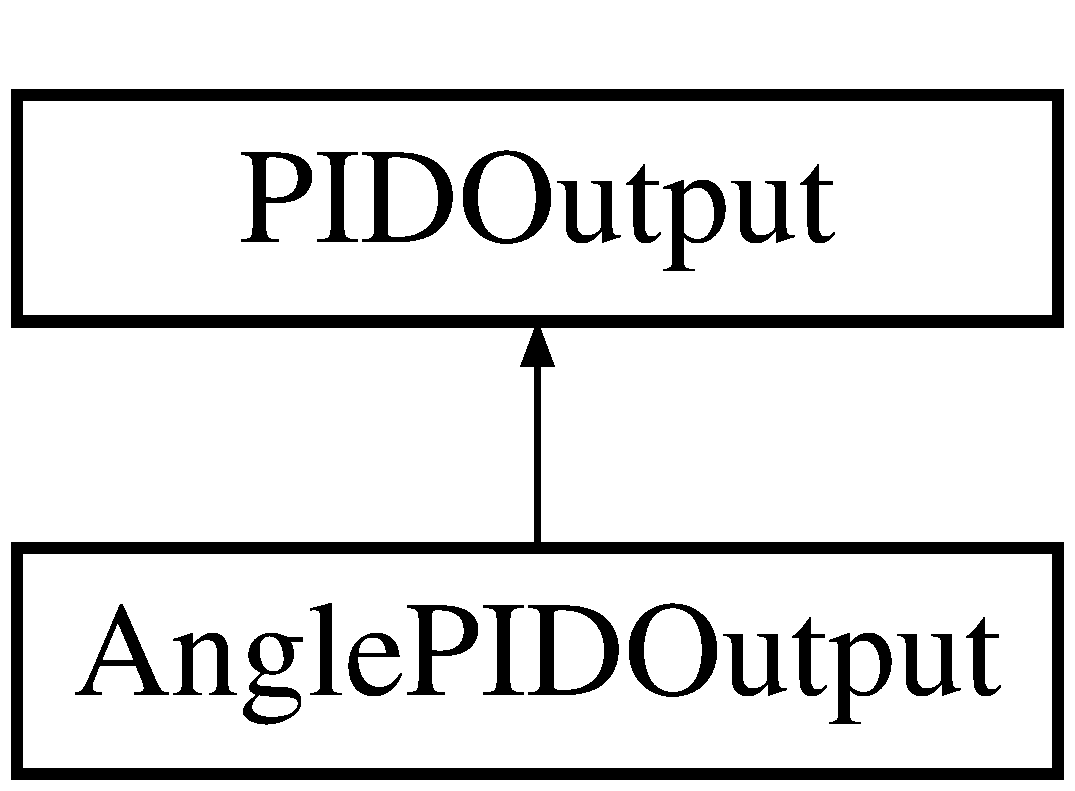
\includegraphics[height=2.000000cm]{class_angle_p_i_d_output}
\end{center}
\end{figure}
\subsection*{Public Member Functions}
\begin{DoxyCompactItemize}
\item 
\mbox{\Hypertarget{class_angle_p_i_d_output_a2e86b8426e4e2c4e0c04343cf7f6a786}\label{class_angle_p_i_d_output_a2e86b8426e4e2c4e0c04343cf7f6a786}} 
void {\bfseries P\+I\+D\+Write} (double output)
\item 
\mbox{\Hypertarget{class_angle_p_i_d_output_a405e91653c027b3df6e387ea5987f095}\label{class_angle_p_i_d_output_a405e91653c027b3df6e387ea5987f095}} 
double {\bfseries Get\+P\+I\+D\+Output} ()
\end{DoxyCompactItemize}
\subsection*{Private Attributes}
\begin{DoxyCompactItemize}
\item 
\mbox{\Hypertarget{class_angle_p_i_d_output_a0cedb94e093c1e5f4b71de6b8b8974ab}\label{class_angle_p_i_d_output_a0cedb94e093c1e5f4b71de6b8b8974ab}} 
double {\bfseries pid\+Output\+\_\+}
\end{DoxyCompactItemize}


The documentation for this class was generated from the following files\+:\begin{DoxyCompactItemize}
\item 
/\+Users/maggiewang/\+Space\+\_\+\+Cookies/spacecookies/frc2017/src/\+Auto/\+Commands/Drive\+Straight\+Command.\+h\item 
/\+Users/maggiewang/\+Space\+\_\+\+Cookies/spacecookies/frc2017/src/\+Auto/\+Commands/Drive\+Straight\+Command.\+cpp\end{DoxyCompactItemize}

\hypertarget{class_auto_command}{}\section{Auto\+Command Class Reference}
\label{class_auto_command}\index{Auto\+Command@{Auto\+Command}}
Inheritance diagram for Auto\+Command\+:\begin{figure}[H]
\begin{center}
\leavevmode
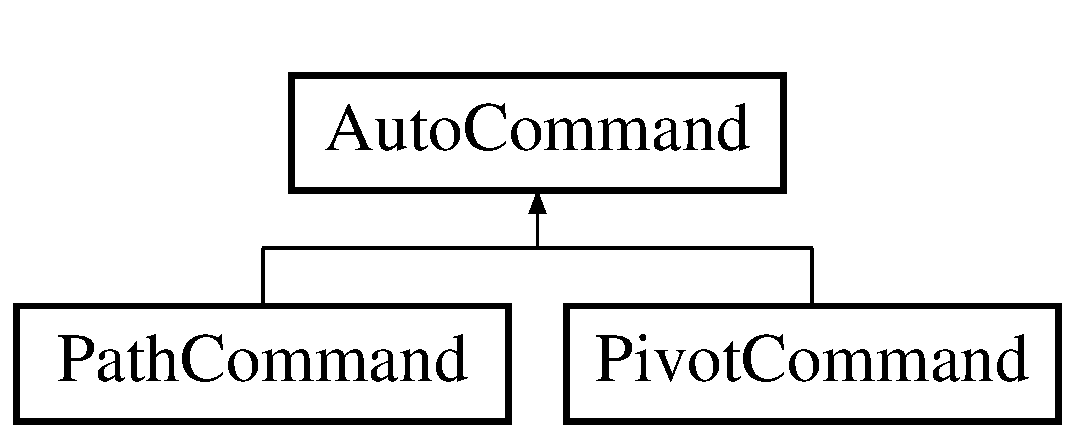
\includegraphics[height=2.000000cm]{class_auto_command}
\end{center}
\end{figure}
\subsection*{Public Member Functions}
\begin{DoxyCompactItemize}
\item 
\mbox{\Hypertarget{class_auto_command_a55e2d94651b71b68589629fb9e5b5e64}\label{class_auto_command_a55e2d94651b71b68589629fb9e5b5e64}} 
virtual void {\bfseries Init} ()=0
\item 
\mbox{\Hypertarget{class_auto_command_ae396d1857033236f2e1864ea0fff0f69}\label{class_auto_command_ae396d1857033236f2e1864ea0fff0f69}} 
virtual void {\bfseries Update} (double curr\+Time\+Sec, double delta\+Time\+Sec)=0
\item 
\mbox{\Hypertarget{class_auto_command_af2a035dbde9903b13b6500f2801ad0be}\label{class_auto_command_af2a035dbde9903b13b6500f2801ad0be}} 
virtual bool {\bfseries Is\+Done} ()=0
\item 
\mbox{\Hypertarget{class_auto_command_a13df47b2b27505a229670f1558491473}\label{class_auto_command_a13df47b2b27505a229670f1558491473}} 
\hyperlink{class_auto_command}{Auto\+Command} $\ast$ {\bfseries Get\+Next\+Command} ()
\item 
\mbox{\Hypertarget{class_auto_command_a339b50cd26f092f84c27b06493f320f0}\label{class_auto_command_a339b50cd26f092f84c27b06493f320f0}} 
void {\bfseries Set\+Next\+Command} (\hyperlink{class_auto_command}{Auto\+Command} $\ast$my\+Next\+Command)
\end{DoxyCompactItemize}
\subsection*{Private Attributes}
\begin{DoxyCompactItemize}
\item 
\mbox{\Hypertarget{class_auto_command_a408872b0525fc1b6296d10727612c848}\label{class_auto_command_a408872b0525fc1b6296d10727612c848}} 
\hyperlink{class_auto_command}{Auto\+Command} $\ast$ {\bfseries next\+Command}
\end{DoxyCompactItemize}


The documentation for this class was generated from the following file\+:\begin{DoxyCompactItemize}
\item 
/\+Users/maggiewang/\+Space\+\_\+\+Cookies/spacecookies/frc2017/src/\+Auto/\+Commands/Auto\+Command.\+h\end{DoxyCompactItemize}

\hypertarget{class_auto_controller}{}\section{Auto\+Controller Class Reference}
\label{class_auto_controller}\index{Auto\+Controller@{Auto\+Controller}}
\subsection*{Public Member Functions}
\begin{DoxyCompactItemize}
\item 
\mbox{\Hypertarget{class_auto_controller_a8fddf9163735e6fc44572e9f59116084}\label{class_auto_controller_a8fddf9163735e6fc44572e9f59116084}} 
{\bfseries Auto\+Controller} (\hyperlink{class_auto_mode}{Auto\+Mode} $\ast$auto\+Mode)
\item 
\mbox{\Hypertarget{class_auto_controller_a8bb1c3117bf7e528c73e4d3edd49d0ba}\label{class_auto_controller_a8bb1c3117bf7e528c73e4d3edd49d0ba}} 
void {\bfseries Set\+Autonomous\+Mode} (\hyperlink{class_auto_mode}{Auto\+Mode} $\ast$auto\+Mode)
\item 
\mbox{\Hypertarget{class_auto_controller_a86c89bedf59d9746d729dead3368460f}\label{class_auto_controller_a86c89bedf59d9746d729dead3368460f}} 
void {\bfseries Start\+Autonomous} ()
\item 
\mbox{\Hypertarget{class_auto_controller_a8b7b16e449078e1818b4bc302f97da07}\label{class_auto_controller_a8b7b16e449078e1818b4bc302f97da07}} 
void {\bfseries Init} ()
\item 
\mbox{\Hypertarget{class_auto_controller_a733fa15c9d374adcb458b0d6f0890910}\label{class_auto_controller_a733fa15c9d374adcb458b0d6f0890910}} 
void {\bfseries Update} (double curr\+Time\+Sec, double delta\+Time\+Sec)
\item 
\mbox{\Hypertarget{class_auto_controller_a58a880e7fdce5953714c3a1d70f49eac}\label{class_auto_controller_a58a880e7fdce5953714c3a1d70f49eac}} 
void {\bfseries Reset} ()
\item 
\mbox{\Hypertarget{class_auto_controller_a692f9395f78cb214ed7c410505686334}\label{class_auto_controller_a692f9395f78cb214ed7c410505686334}} 
bool {\bfseries Is\+Done} ()
\end{DoxyCompactItemize}
\subsection*{Private Attributes}
\begin{DoxyCompactItemize}
\item 
\mbox{\Hypertarget{class_auto_controller_a85f5b014c905fe3ac77e3024ad1ebe56}\label{class_auto_controller_a85f5b014c905fe3ac77e3024ad1ebe56}} 
\hyperlink{class_auto_mode}{Auto\+Mode} $\ast$ {\bfseries auto\+Mode}
\end{DoxyCompactItemize}


The documentation for this class was generated from the following files\+:\begin{DoxyCompactItemize}
\item 
/\+Users/maggiewang/\+Space\+\_\+\+Cookies/spacecookies/frc2017/src/\+Auto/Auto\+Controller.\+h\item 
/\+Users/maggiewang/\+Space\+\_\+\+Cookies/spacecookies/frc2017/src/\+Auto/Auto\+Controller.\+cpp\end{DoxyCompactItemize}

\hypertarget{class_auto_mode}{}\section{Auto\+Mode Class Reference}
\label{class_auto_mode}\index{Auto\+Mode@{Auto\+Mode}}
Inheritance diagram for Auto\+Mode\+:\begin{figure}[H]
\begin{center}
\leavevmode
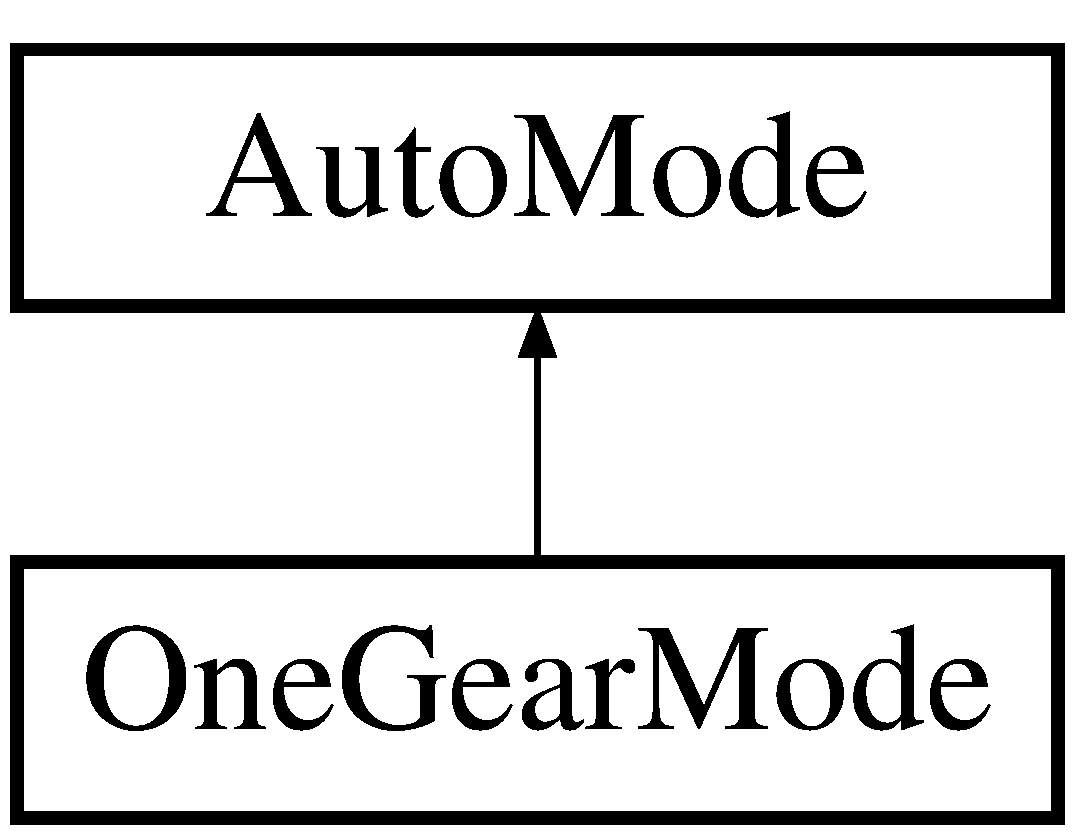
\includegraphics[height=2.000000cm]{class_auto_mode}
\end{center}
\end{figure}
\subsection*{Public Member Functions}
\begin{DoxyCompactItemize}
\item 
\mbox{\Hypertarget{class_auto_mode_a71d5383a52a2e1d29548099d86ae66b6}\label{class_auto_mode_a71d5383a52a2e1d29548099d86ae66b6}} 
virtual void {\bfseries Create\+Queue} ()=0
\item 
\mbox{\Hypertarget{class_auto_mode_ae30ad1e90a36975db5b1bd6d0d764408}\label{class_auto_mode_ae30ad1e90a36975db5b1bd6d0d764408}} 
virtual void {\bfseries Init} ()=0
\item 
void \hyperlink{class_auto_mode_af5eb2f835e2712588986ca8fd9a8735a}{Update} (double curr\+Time\+Sec, double delta\+Time\+Sec)
\item 
\mbox{\Hypertarget{class_auto_mode_acb6a8d7e9e3635dd1d0af27297fe045f}\label{class_auto_mode_acb6a8d7e9e3635dd1d0af27297fe045f}} 
virtual void {\bfseries Refresh\+Ini} ()=0
\item 
bool \hyperlink{class_auto_mode_a6f734a1af959e284fced7666e397bf65}{Is\+Done} ()
\end{DoxyCompactItemize}
\subsection*{Protected Attributes}
\begin{DoxyCompactItemize}
\item 
\mbox{\Hypertarget{class_auto_mode_acaf4e4b36bbc309c6fae4cdac56b38d3}\label{class_auto_mode_acaf4e4b36bbc309c6fae4cdac56b38d3}} 
\hyperlink{class_auto_command}{Auto\+Command} $\ast$ {\bfseries current\+Command}
\end{DoxyCompactItemize}


\subsection{Member Function Documentation}
\mbox{\Hypertarget{class_auto_mode_a6f734a1af959e284fced7666e397bf65}\label{class_auto_mode_a6f734a1af959e284fced7666e397bf65}} 
\index{Auto\+Mode@{Auto\+Mode}!Is\+Done@{Is\+Done}}
\index{Is\+Done@{Is\+Done}!Auto\+Mode@{Auto\+Mode}}
\subsubsection{\texorpdfstring{Is\+Done()}{IsDone()}}
{\footnotesize\ttfamily bool Auto\+Mode\+::\+Is\+Done (\begin{DoxyParamCaption}{ }\end{DoxyParamCaption})\hspace{0.3cm}{\ttfamily [inline]}}

Returns when \hyperlink{class_auto_mode}{Auto\+Mode} is done \begin{DoxyReturn}{Returns}
true if there is no current command or current command is N\+U\+LL 
\end{DoxyReturn}
\mbox{\Hypertarget{class_auto_mode_af5eb2f835e2712588986ca8fd9a8735a}\label{class_auto_mode_af5eb2f835e2712588986ca8fd9a8735a}} 
\index{Auto\+Mode@{Auto\+Mode}!Update@{Update}}
\index{Update@{Update}!Auto\+Mode@{Auto\+Mode}}
\subsubsection{\texorpdfstring{Update()}{Update()}}
{\footnotesize\ttfamily void Auto\+Mode\+::\+Update (\begin{DoxyParamCaption}\item[{double}]{curr\+Time\+Sec,  }\item[{double}]{delta\+Time\+Sec }\end{DoxyParamCaption})\hspace{0.3cm}{\ttfamily [inline]}}

Updates the current command and prints out if each command is complete and also if the automode update is finished 
\begin{DoxyParams}{Parameters}
{\em curr\+Time\+Sec} & a double current time \\
\hline
{\em delta\+Time\+Sec} & a double how often to update \\
\hline
\end{DoxyParams}


The documentation for this class was generated from the following file\+:\begin{DoxyCompactItemize}
\item 
/\+Users/maggiewang/\+Space\+\_\+\+Cookies/spacecookies/frc2017/src/\+Auto/\+Modes/Auto\+Mode.\+h\end{DoxyCompactItemize}

\hypertarget{class_blank_mode}{}\section{Blank\+Mode Class Reference}
\label{class_blank_mode}\index{Blank\+Mode@{Blank\+Mode}}


The documentation for this class was generated from the following files\+:\begin{DoxyCompactItemize}
\item 
/\+Users/maggiewang/\+Space\+\_\+\+Cookies/spacecookies/frc2017/src/\+Auto/\+Modes/Blank\+Mode.\+h\item 
/\+Users/maggiewang/\+Space\+\_\+\+Cookies/spacecookies/frc2017/src/\+Auto/\+Modes/Blank\+Mode.\+cpp\end{DoxyCompactItemize}

\hypertarget{class_button_reader}{}\section{Button\+Reader Class Reference}
\label{class_button_reader}\index{Button\+Reader@{Button\+Reader}}
Inheritance diagram for Button\+Reader\+:\begin{figure}[H]
\begin{center}
\leavevmode
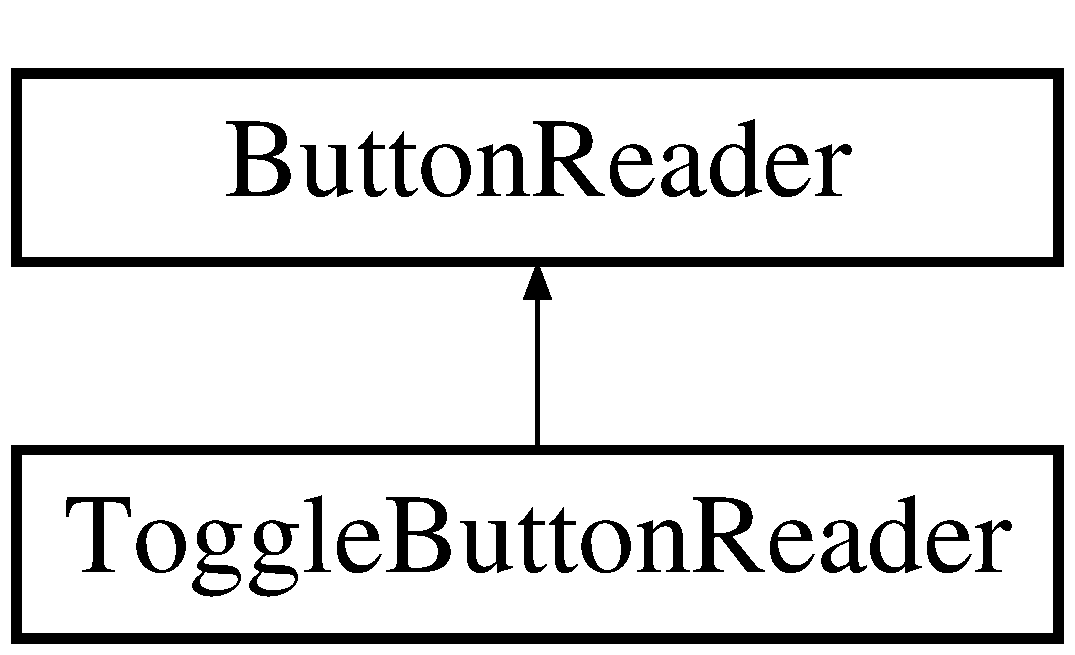
\includegraphics[height=2.000000cm]{class_button_reader}
\end{center}
\end{figure}
\subsection*{Public Member Functions}
\begin{DoxyCompactItemize}
\item 
\hyperlink{class_button_reader_a1bb75f75d6e392a748c6101e09e3bd3c}{Button\+Reader} (Joystick $\ast$joy, int button\+Num)
\item 
void \hyperlink{class_button_reader_a4585d7ca717ea49021ac5a786c352b81}{Read\+Value} ()
\item 
bool \hyperlink{class_button_reader_a89a81fffd0726973811c6e791ac12a1d}{Is\+Down} ()
\item 
bool \hyperlink{class_button_reader_ace4a07bf7f65418c026477b9d5ab1225}{Was\+Just\+Pressed} ()
\item 
bool \hyperlink{class_button_reader_afded4de61711a165928fe0730d8743e7}{Was\+Just\+Released} ()
\item 
bool \hyperlink{class_button_reader_a2c19cae72a053bbba95f1c1a91735876}{State\+Just\+Changed} ()
\end{DoxyCompactItemize}
\subsection*{Private Attributes}
\begin{DoxyCompactItemize}
\item 
\mbox{\Hypertarget{class_button_reader_aac4f8ee19043c203be56abf375e8b319}\label{class_button_reader_aac4f8ee19043c203be56abf375e8b319}} 
Joystick $\ast$ {\bfseries joystick}
\item 
\mbox{\Hypertarget{class_button_reader_a92bac462d8bc6ee16fea40c13ff50e95}\label{class_button_reader_a92bac462d8bc6ee16fea40c13ff50e95}} 
int {\bfseries button\+Num}
\item 
\mbox{\Hypertarget{class_button_reader_a6fab0789d8dd7b5c424e7fa3c12d4ca9}\label{class_button_reader_a6fab0789d8dd7b5c424e7fa3c12d4ca9}} 
bool {\bfseries last\+State}
\item 
\mbox{\Hypertarget{class_button_reader_a1d139e4dbe81f6b1942b5f74c56b6492}\label{class_button_reader_a1d139e4dbe81f6b1942b5f74c56b6492}} 
bool {\bfseries curr\+State}
\end{DoxyCompactItemize}


\subsection{Constructor \& Destructor Documentation}
\mbox{\Hypertarget{class_button_reader_a1bb75f75d6e392a748c6101e09e3bd3c}\label{class_button_reader_a1bb75f75d6e392a748c6101e09e3bd3c}} 
\index{Button\+Reader@{Button\+Reader}!Button\+Reader@{Button\+Reader}}
\index{Button\+Reader@{Button\+Reader}!Button\+Reader@{Button\+Reader}}
\subsubsection{\texorpdfstring{Button\+Reader()}{ButtonReader()}}
{\footnotesize\ttfamily Button\+Reader\+::\+Button\+Reader (\begin{DoxyParamCaption}\item[{Joystick $\ast$}]{joy,  }\item[{int}]{button\+Num }\end{DoxyParamCaption})}

Sets joystick, button, gets curr\+State from rawbutton, sets last state to curr\+State 

\subsection{Member Function Documentation}
\mbox{\Hypertarget{class_button_reader_a89a81fffd0726973811c6e791ac12a1d}\label{class_button_reader_a89a81fffd0726973811c6e791ac12a1d}} 
\index{Button\+Reader@{Button\+Reader}!Is\+Down@{Is\+Down}}
\index{Is\+Down@{Is\+Down}!Button\+Reader@{Button\+Reader}}
\subsubsection{\texorpdfstring{Is\+Down()}{IsDown()}}
{\footnotesize\ttfamily bool Button\+Reader\+::\+Is\+Down (\begin{DoxyParamCaption}{ }\end{DoxyParamCaption})}

\begin{DoxyReturn}{Returns}
current state of button (whether its currently pressed) 
\end{DoxyReturn}
\mbox{\Hypertarget{class_button_reader_a4585d7ca717ea49021ac5a786c352b81}\label{class_button_reader_a4585d7ca717ea49021ac5a786c352b81}} 
\index{Button\+Reader@{Button\+Reader}!Read\+Value@{Read\+Value}}
\index{Read\+Value@{Read\+Value}!Button\+Reader@{Button\+Reader}}
\subsubsection{\texorpdfstring{Read\+Value()}{ReadValue()}}
{\footnotesize\ttfamily void Button\+Reader\+::\+Read\+Value (\begin{DoxyParamCaption}{ }\end{DoxyParamCaption})}

Sets last\+State to curr\+State, updates curr\+State w/button \mbox{\Hypertarget{class_button_reader_a2c19cae72a053bbba95f1c1a91735876}\label{class_button_reader_a2c19cae72a053bbba95f1c1a91735876}} 
\index{Button\+Reader@{Button\+Reader}!State\+Just\+Changed@{State\+Just\+Changed}}
\index{State\+Just\+Changed@{State\+Just\+Changed}!Button\+Reader@{Button\+Reader}}
\subsubsection{\texorpdfstring{State\+Just\+Changed()}{StateJustChanged()}}
{\footnotesize\ttfamily bool Button\+Reader\+::\+State\+Just\+Changed (\begin{DoxyParamCaption}{ }\end{DoxyParamCaption})}

\begin{DoxyReturn}{Returns}
true if last\+State doesn\textquotesingle{}t equal curr\+State. else return false. 
\end{DoxyReturn}
\mbox{\Hypertarget{class_button_reader_ace4a07bf7f65418c026477b9d5ab1225}\label{class_button_reader_ace4a07bf7f65418c026477b9d5ab1225}} 
\index{Button\+Reader@{Button\+Reader}!Was\+Just\+Pressed@{Was\+Just\+Pressed}}
\index{Was\+Just\+Pressed@{Was\+Just\+Pressed}!Button\+Reader@{Button\+Reader}}
\subsubsection{\texorpdfstring{Was\+Just\+Pressed()}{WasJustPressed()}}
{\footnotesize\ttfamily bool Button\+Reader\+::\+Was\+Just\+Pressed (\begin{DoxyParamCaption}{ }\end{DoxyParamCaption})}

\begin{DoxyReturn}{Returns}
true if last\+State is true and curr\+State is false. else returns false. 
\end{DoxyReturn}
\mbox{\Hypertarget{class_button_reader_afded4de61711a165928fe0730d8743e7}\label{class_button_reader_afded4de61711a165928fe0730d8743e7}} 
\index{Button\+Reader@{Button\+Reader}!Was\+Just\+Released@{Was\+Just\+Released}}
\index{Was\+Just\+Released@{Was\+Just\+Released}!Button\+Reader@{Button\+Reader}}
\subsubsection{\texorpdfstring{Was\+Just\+Released()}{WasJustReleased()}}
{\footnotesize\ttfamily bool Button\+Reader\+::\+Was\+Just\+Released (\begin{DoxyParamCaption}{ }\end{DoxyParamCaption})}

\begin{DoxyReturn}{Returns}
true if last\+State is false and curr\+State is true. else returns false. 
\end{DoxyReturn}


The documentation for this class was generated from the following files\+:\begin{DoxyCompactItemize}
\item 
/\+Users/maggiewang/\+Space\+\_\+\+Cookies/spacecookies/frc2017/src/\+Driver\+Station/Button\+Reader.\+h\item 
/\+Users/maggiewang/\+Space\+\_\+\+Cookies/spacecookies/frc2017/src/\+Driver\+Station/Button\+Reader.\+cpp\end{DoxyCompactItemize}

\hypertarget{class_control_board}{}\section{Control\+Board Class Reference}
\label{class_control_board}\index{Control\+Board@{Control\+Board}}
Inheritance diagram for Control\+Board\+:\begin{figure}[H]
\begin{center}
\leavevmode
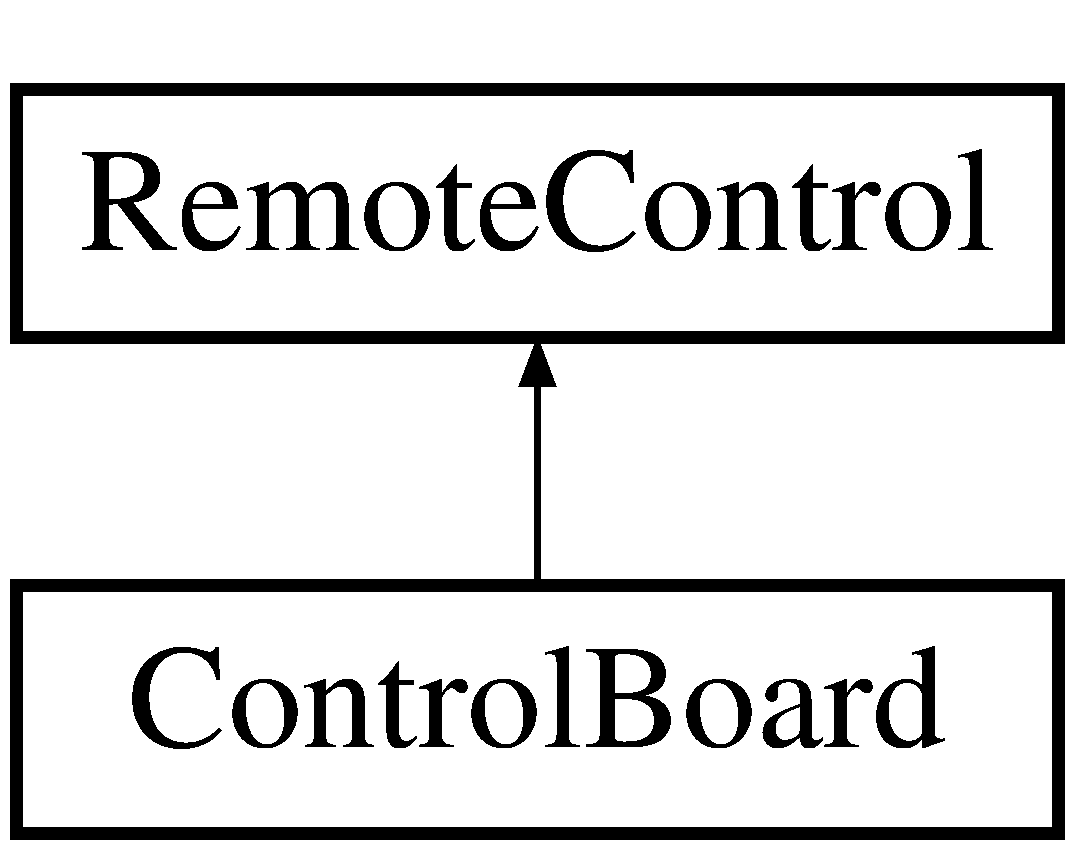
\includegraphics[height=2.000000cm]{class_control_board}
\end{center}
\end{figure}
\subsection*{Public Member Functions}
\begin{DoxyCompactItemize}
\item 
\mbox{\Hypertarget{class_control_board_abc38ec1feb7a7c38adfe7ced04fc5a79}\label{class_control_board_abc38ec1feb7a7c38adfe7ced04fc5a79}} 
void {\bfseries Read\+Controls} ()
\item 
\mbox{\Hypertarget{class_control_board_a82d4f6abff67ad0ba60b263d65fcc924}\label{class_control_board_a82d4f6abff67ad0ba60b263d65fcc924}} 
double {\bfseries Get\+Joystick\+Value} (Joysticks j, Axes a)
\item 
\mbox{\Hypertarget{class_control_board_a53f6a067fdec6785017465dba9ee2be6}\label{class_control_board_a53f6a067fdec6785017465dba9ee2be6}} 
bool {\bfseries Get\+Reverse\+Drive\+Desired} ()
\item 
\mbox{\Hypertarget{class_control_board_a49f9d98f58c8f8eb8030910c27b187ed}\label{class_control_board_a49f9d98f58c8f8eb8030910c27b187ed}} 
bool {\bfseries Get\+Gear\+Shift\+Desired} ()
\item 
\mbox{\Hypertarget{class_control_board_ab32a6888112f807dff75acbb641a3517}\label{class_control_board_ab32a6888112f807dff75acbb641a3517}} 
bool {\bfseries Get\+Arcade\+Drive\+Desired} ()
\item 
\mbox{\Hypertarget{class_control_board_ac43151ba49812cc42028c957506a4cc4}\label{class_control_board_ac43151ba49812cc42028c957506a4cc4}} 
bool {\bfseries Get\+Quick\+Turn\+Desired} ()
\end{DoxyCompactItemize}
\subsection*{Private Member Functions}
\begin{DoxyCompactItemize}
\item 
\mbox{\Hypertarget{class_control_board_a119aafaac10209d3a0ed71a3ecbf0a8a}\label{class_control_board_a119aafaac10209d3a0ed71a3ecbf0a8a}} 
void {\bfseries Read\+All\+Buttons} ()
\end{DoxyCompactItemize}
\subsection*{Private Attributes}
\begin{DoxyCompactItemize}
\item 
\mbox{\Hypertarget{class_control_board_aa416e9616eb5e9650274fe609deef35a}\label{class_control_board_aa416e9616eb5e9650274fe609deef35a}} 
double {\bfseries left\+Joy\+X\+\_\+}
\item 
\mbox{\Hypertarget{class_control_board_a62d7b23bd7d3a4d1362d13b67ed706b1}\label{class_control_board_a62d7b23bd7d3a4d1362d13b67ed706b1}} 
double {\bfseries left\+Joy\+Y\+\_\+}
\item 
\mbox{\Hypertarget{class_control_board_a4c2f86c6e0dac63ed07a8a8e0ff08f96}\label{class_control_board_a4c2f86c6e0dac63ed07a8a8e0ff08f96}} 
double {\bfseries right\+Joy\+X\+\_\+}
\item 
\mbox{\Hypertarget{class_control_board_aae31045f2a49fdd74bf149529dd3ad4d}\label{class_control_board_aae31045f2a49fdd74bf149529dd3ad4d}} 
double {\bfseries right\+Joy\+Y\+\_\+}
\item 
\mbox{\Hypertarget{class_control_board_a9801f6d198aba04809ceae4226d37e31}\label{class_control_board_a9801f6d198aba04809ceae4226d37e31}} 
bool {\bfseries reverse\+Drive\+Desired\+\_\+}
\item 
\mbox{\Hypertarget{class_control_board_ad7999d7ba82292494c4672ea512e3b9e}\label{class_control_board_ad7999d7ba82292494c4672ea512e3b9e}} 
bool {\bfseries gear\+Shift\+Desired\+\_\+}
\item 
\mbox{\Hypertarget{class_control_board_a78bd6b9dda2e0035527b16f35a09c5ae}\label{class_control_board_a78bd6b9dda2e0035527b16f35a09c5ae}} 
bool {\bfseries arcade\+Drive\+Desired\+\_\+}
\item 
\mbox{\Hypertarget{class_control_board_a59b412d2fab63ecd421419bec6710d5d}\label{class_control_board_a59b412d2fab63ecd421419bec6710d5d}} 
bool {\bfseries quick\+Turn\+Desired\+\_\+}
\item 
\mbox{\Hypertarget{class_control_board_a3d1d2b17bf6a2290271d6fba94fb20e2}\label{class_control_board_a3d1d2b17bf6a2290271d6fba94fb20e2}} 
Joystick $\ast$ {\bfseries left\+Joy\+\_\+}
\item 
\mbox{\Hypertarget{class_control_board_a9f99e67fc5be70b7a242b489d106e6e4}\label{class_control_board_a9f99e67fc5be70b7a242b489d106e6e4}} 
Joystick $\ast$ {\bfseries right\+Joy\+\_\+}
\item 
\mbox{\Hypertarget{class_control_board_a32d6c4eeaf66d97bd1c407bbaccebb0b}\label{class_control_board_a32d6c4eeaf66d97bd1c407bbaccebb0b}} 
Joystick $\ast$ {\bfseries operator\+Joy\+\_\+}
\item 
\mbox{\Hypertarget{class_control_board_a862917fc3f42591da7f743cb5a474f69}\label{class_control_board_a862917fc3f42591da7f743cb5a474f69}} 
Joystick $\ast$ {\bfseries operator\+Joy\+B\+\_\+}
\item 
\mbox{\Hypertarget{class_control_board_a2bc303faf6f560ee5bc50740d531087f}\label{class_control_board_a2bc303faf6f560ee5bc50740d531087f}} 
\hyperlink{class_button_reader}{Button\+Reader} $\ast$ {\bfseries drive\+Direction\+Button}
\item 
\mbox{\Hypertarget{class_control_board_a169abc98da7af2228d32e6af40b59618}\label{class_control_board_a169abc98da7af2228d32e6af40b59618}} 
\hyperlink{class_button_reader}{Button\+Reader} $\ast$ {\bfseries gear\+Shift\+Button}
\item 
\mbox{\Hypertarget{class_control_board_a85921de97d4183cfb321f6dfb3aa09a6}\label{class_control_board_a85921de97d4183cfb321f6dfb3aa09a6}} 
\hyperlink{class_button_reader}{Button\+Reader} $\ast$ {\bfseries arcade\+Drive\+Button}
\item 
\mbox{\Hypertarget{class_control_board_a7f00556cbd9514ab50e79fd202187b27}\label{class_control_board_a7f00556cbd9514ab50e79fd202187b27}} 
\hyperlink{class_button_reader}{Button\+Reader} $\ast$ {\bfseries quick\+Turn\+Button}
\end{DoxyCompactItemize}
\subsection*{Additional Inherited Members}


The documentation for this class was generated from the following files\+:\begin{DoxyCompactItemize}
\item 
/\+Users/maggiewang/\+Space\+\_\+\+Cookies/spacecookies/frc2017/src/\+Driver\+Station/Control\+Board.\+h\item 
/\+Users/maggiewang/\+Space\+\_\+\+Cookies/spacecookies/frc2017/src/\+Driver\+Station/Control\+Board.\+cpp\end{DoxyCompactItemize}

\hypertarget{class_distance_p_i_d_output}{}\section{Distance\+P\+I\+D\+Output Class Reference}
\label{class_distance_p_i_d_output}\index{Distance\+P\+I\+D\+Output@{Distance\+P\+I\+D\+Output}}
Inheritance diagram for Distance\+P\+I\+D\+Output\+:\begin{figure}[H]
\begin{center}
\leavevmode
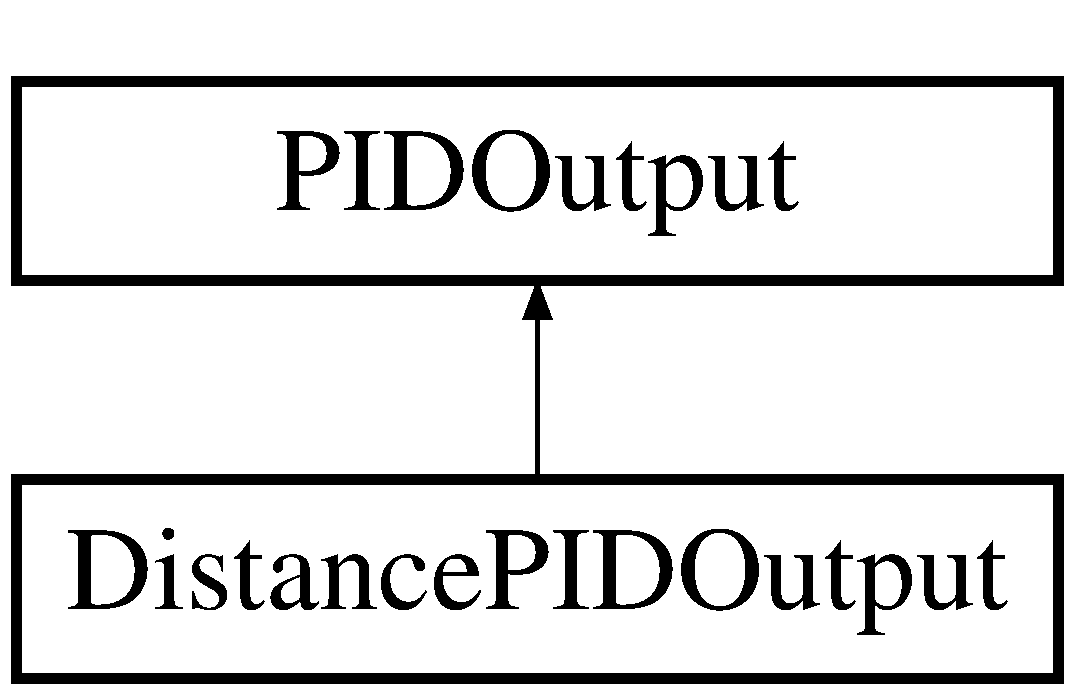
\includegraphics[height=2.000000cm]{class_distance_p_i_d_output}
\end{center}
\end{figure}
\subsection*{Public Member Functions}
\begin{DoxyCompactItemize}
\item 
\mbox{\Hypertarget{class_distance_p_i_d_output_abb33d2e1fc125644341d840c1b742102}\label{class_distance_p_i_d_output_abb33d2e1fc125644341d840c1b742102}} 
void {\bfseries P\+I\+D\+Write} (double output)
\item 
\mbox{\Hypertarget{class_distance_p_i_d_output_a0c391cfc3f7d9435eef3e325e8eb60ec}\label{class_distance_p_i_d_output_a0c391cfc3f7d9435eef3e325e8eb60ec}} 
double {\bfseries Get\+P\+I\+D\+Output} ()
\end{DoxyCompactItemize}
\subsection*{Private Attributes}
\begin{DoxyCompactItemize}
\item 
\mbox{\Hypertarget{class_distance_p_i_d_output_a1702f9370542e768153841bdc837495a}\label{class_distance_p_i_d_output_a1702f9370542e768153841bdc837495a}} 
double {\bfseries pid\+Output\+\_\+}
\end{DoxyCompactItemize}


The documentation for this class was generated from the following files\+:\begin{DoxyCompactItemize}
\item 
/\+Users/maggiewang/\+Space\+\_\+\+Cookies/spacecookies/frc2017/src/\+Auto/\+Commands/Drive\+Straight\+Command.\+h\item 
/\+Users/maggiewang/\+Space\+\_\+\+Cookies/spacecookies/frc2017/src/\+Auto/\+Commands/Drive\+Straight\+Command.\+cpp\end{DoxyCompactItemize}

\hypertarget{class_drive_controller}{}\section{Drive\+Controller Class Reference}
\label{class_drive_controller}\index{Drive\+Controller@{Drive\+Controller}}
\subsection*{Public Types}
\begin{DoxyCompactItemize}
\item 
\mbox{\Hypertarget{class_drive_controller_abb183068492c689edb76fe802a4a35ad}\label{class_drive_controller_abb183068492c689edb76fe802a4a35ad}} 
enum {\bfseries Drive\+State} \{ {\bfseries k\+Initialize}, 
{\bfseries k\+Teleop\+Drive}, 
{\bfseries k\+Motion\+Profile}
 \}
\end{DoxyCompactItemize}
\subsection*{Public Member Functions}
\begin{DoxyCompactItemize}
\item 
\hyperlink{class_drive_controller_a166bb5ed50199d8482ebbc0e244742a1}{Drive\+Controller} (\hyperlink{class_robot_model}{Robot\+Model} $\ast$robot, \hyperlink{class_control_board}{Control\+Board} $\ast$human\+Control)
\item 
\mbox{\Hypertarget{class_drive_controller_afb1d02465d9feb19335db06c6d686552}\label{class_drive_controller_afb1d02465d9feb19335db06c6d686552}} 
void {\bfseries Reset} ()
\item 
\mbox{\Hypertarget{class_drive_controller_a80935e19c13c8f9212054af0183e53ad}\label{class_drive_controller_a80935e19c13c8f9212054af0183e53ad}} 
void {\bfseries Update\+Motion\+Profile} ()
\item 
void \hyperlink{class_drive_controller_aefc9e8cbe2948d2e72987e0a8a2cbf80}{Update} (double curr\+Time\+Sec, double delta\+Time\+Sec)
\item 
bool \hyperlink{class_drive_controller_ae07d828e9b1738bd0baf6dca46e5bd5c}{Is\+Done} ()
\item 
\mbox{\Hypertarget{class_drive_controller_abbcf50b6d01eda0d1a45131dfeb97db8}\label{class_drive_controller_abbcf50b6d01eda0d1a45131dfeb97db8}} 
void {\bfseries Print\+Drive\+Values} ()
\end{DoxyCompactItemize}
\subsection*{Private Member Functions}
\begin{DoxyCompactItemize}
\item 
void \hyperlink{class_drive_controller_a59d4b701fd83e101a3aaf9726fc626dd}{Arcade\+Drive} (double myX, double myY)
\item 
void \hyperlink{class_drive_controller_a93ed2c0196329dcbd6dd666f609ef487}{Tank\+Drive} (double Left, double Right)
\item 
void \hyperlink{class_drive_controller_a3e9f778228ea2812b372fbb43fdf5a08}{Quick\+Turn} (double my\+Right)
\item 
int \hyperlink{class_drive_controller_aeecbfd3643cadb19cc30af0f22c41c98}{Drive\+Direction} ()
\item 
int \hyperlink{class_drive_controller_a001ab748cefcfdb9d4aa10b3cf699d53}{Get\+Drive\+State} ()
\end{DoxyCompactItemize}
\subsection*{Private Attributes}
\begin{DoxyCompactItemize}
\item 
\mbox{\Hypertarget{class_drive_controller_abc5ee587234574826c58a259902fa86f}\label{class_drive_controller_abc5ee587234574826c58a259902fa86f}} 
\hyperlink{class_robot_model}{Robot\+Model} $\ast$ {\bfseries robot\+\_\+}
\item 
\mbox{\Hypertarget{class_drive_controller_af9b33cc9fd301b54d3cdb31223d8216a}\label{class_drive_controller_af9b33cc9fd301b54d3cdb31223d8216a}} 
\hyperlink{class_control_board}{Control\+Board} $\ast$ {\bfseries human\+Control\+\_\+}
\item 
\mbox{\Hypertarget{class_drive_controller_ad71cbf0f66adf918dba524662867775f}\label{class_drive_controller_ad71cbf0f66adf918dba524662867775f}} 
bool {\bfseries is\+Done\+\_\+}
\item 
\mbox{\Hypertarget{class_drive_controller_ac8e6cfbda24abc7c033e6ec9c2f75f13}\label{class_drive_controller_ac8e6cfbda24abc7c033e6ec9c2f75f13}} 
uint32\+\_\+t {\bfseries curr\+State\+\_\+}
\item 
\mbox{\Hypertarget{class_drive_controller_abc8e83a004bdf2edd3b76aeb7d5b66d2}\label{class_drive_controller_abc8e83a004bdf2edd3b76aeb7d5b66d2}} 
uint32\+\_\+t {\bfseries next\+State\+\_\+}
\end{DoxyCompactItemize}


\subsection{Constructor \& Destructor Documentation}
\mbox{\Hypertarget{class_drive_controller_a166bb5ed50199d8482ebbc0e244742a1}\label{class_drive_controller_a166bb5ed50199d8482ebbc0e244742a1}} 
\index{Drive\+Controller@{Drive\+Controller}!Drive\+Controller@{Drive\+Controller}}
\index{Drive\+Controller@{Drive\+Controller}!Drive\+Controller@{Drive\+Controller}}
\subsubsection{\texorpdfstring{Drive\+Controller()}{DriveController()}}
{\footnotesize\ttfamily Drive\+Controller\+::\+Drive\+Controller (\begin{DoxyParamCaption}\item[{\hyperlink{class_robot_model}{Robot\+Model} $\ast$}]{robot,  }\item[{\hyperlink{class_control_board}{Control\+Board} $\ast$}]{human\+Control }\end{DoxyParamCaption})}

Sets state of robot and \hyperlink{class_control_board}{Control\+Board} 
\begin{DoxyParams}{Parameters}
{\em robot} & a \hyperlink{class_robot_model}{Robot\+Model} \\
\hline
{\em human\+Control} & a \hyperlink{class_control_board}{Control\+Board} \\
\hline
\end{DoxyParams}


\subsection{Member Function Documentation}
\mbox{\Hypertarget{class_drive_controller_a59d4b701fd83e101a3aaf9726fc626dd}\label{class_drive_controller_a59d4b701fd83e101a3aaf9726fc626dd}} 
\index{Drive\+Controller@{Drive\+Controller}!Arcade\+Drive@{Arcade\+Drive}}
\index{Arcade\+Drive@{Arcade\+Drive}!Drive\+Controller@{Drive\+Controller}}
\subsubsection{\texorpdfstring{Arcade\+Drive()}{ArcadeDrive()}}
{\footnotesize\ttfamily void Drive\+Controller\+::\+Arcade\+Drive (\begin{DoxyParamCaption}\item[{double}]{myX,  }\item[{double}]{myY }\end{DoxyParamCaption})\hspace{0.3cm}{\ttfamily [private]}}

Allows one joystick to make robot turn, while the other joystick alters speed and direction (forwards or backwards) of the robot. Does not allow max\+Output to be greater than 1.\+0 Does not allow robot to turn if thrust is less than 0.\+1 Does not allow robot to drive forwards/backwards if thrust is less than 0.\+2 
\begin{DoxyParams}{Parameters}
{\em myX} & a double rotate value \\
\hline
{\em myY} & a double thrust value (forwards/backwards) \\
\hline
\end{DoxyParams}
\mbox{\Hypertarget{class_drive_controller_aeecbfd3643cadb19cc30af0f22c41c98}\label{class_drive_controller_aeecbfd3643cadb19cc30af0f22c41c98}} 
\index{Drive\+Controller@{Drive\+Controller}!Drive\+Direction@{Drive\+Direction}}
\index{Drive\+Direction@{Drive\+Direction}!Drive\+Controller@{Drive\+Controller}}
\subsubsection{\texorpdfstring{Drive\+Direction()}{DriveDirection()}}
{\footnotesize\ttfamily int Drive\+Controller\+::\+Drive\+Direction (\begin{DoxyParamCaption}{ }\end{DoxyParamCaption})\hspace{0.3cm}{\ttfamily [private]}}

Indicates direction of drive (forwards or backwards) \mbox{\Hypertarget{class_drive_controller_a001ab748cefcfdb9d4aa10b3cf699d53}\label{class_drive_controller_a001ab748cefcfdb9d4aa10b3cf699d53}} 
\index{Drive\+Controller@{Drive\+Controller}!Get\+Drive\+State@{Get\+Drive\+State}}
\index{Get\+Drive\+State@{Get\+Drive\+State}!Drive\+Controller@{Drive\+Controller}}
\subsubsection{\texorpdfstring{Get\+Drive\+State()}{GetDriveState()}}
{\footnotesize\ttfamily int Drive\+Controller\+::\+Get\+Drive\+State (\begin{DoxyParamCaption}{ }\end{DoxyParamCaption})\hspace{0.3cm}{\ttfamily [private]}}

Gets current state of drive \mbox{\Hypertarget{class_drive_controller_ae07d828e9b1738bd0baf6dca46e5bd5c}\label{class_drive_controller_ae07d828e9b1738bd0baf6dca46e5bd5c}} 
\index{Drive\+Controller@{Drive\+Controller}!Is\+Done@{Is\+Done}}
\index{Is\+Done@{Is\+Done}!Drive\+Controller@{Drive\+Controller}}
\subsubsection{\texorpdfstring{Is\+Done()}{IsDone()}}
{\footnotesize\ttfamily bool Drive\+Controller\+::\+Is\+Done (\begin{DoxyParamCaption}{ }\end{DoxyParamCaption})}

\begin{DoxyReturn}{Returns}
whether or not is\+Done is true, gets called in \hyperlink{class_path_command}{Path\+Command} 
\end{DoxyReturn}
\mbox{\Hypertarget{class_drive_controller_a3e9f778228ea2812b372fbb43fdf5a08}\label{class_drive_controller_a3e9f778228ea2812b372fbb43fdf5a08}} 
\index{Drive\+Controller@{Drive\+Controller}!Quick\+Turn@{Quick\+Turn}}
\index{Quick\+Turn@{Quick\+Turn}!Drive\+Controller@{Drive\+Controller}}
\subsubsection{\texorpdfstring{Quick\+Turn()}{QuickTurn()}}
{\footnotesize\ttfamily void Drive\+Controller\+::\+Quick\+Turn (\begin{DoxyParamCaption}\item[{double}]{my\+Right }\end{DoxyParamCaption})\hspace{0.3cm}{\ttfamily [private]}}

Allows robot to turn quickly, at sharp angle 
\begin{DoxyParams}{Parameters}
{\em my\+Right} & a double allows robot to turn right or left \\
\hline
\end{DoxyParams}
\mbox{\Hypertarget{class_drive_controller_a93ed2c0196329dcbd6dd666f609ef487}\label{class_drive_controller_a93ed2c0196329dcbd6dd666f609ef487}} 
\index{Drive\+Controller@{Drive\+Controller}!Tank\+Drive@{Tank\+Drive}}
\index{Tank\+Drive@{Tank\+Drive}!Drive\+Controller@{Drive\+Controller}}
\subsubsection{\texorpdfstring{Tank\+Drive()}{TankDrive()}}
{\footnotesize\ttfamily void Drive\+Controller\+::\+Tank\+Drive (\begin{DoxyParamCaption}\item[{double}]{Left,  }\item[{double}]{Right }\end{DoxyParamCaption})\hspace{0.3cm}{\ttfamily [private]}}

Senses how much each joystick is pushed and uses values to turn wheels 
\begin{DoxyParams}{Parameters}
{\em Left} & a double how much left joystick is pushed \\
\hline
{\em Right} & a double how much right joystick is pushed \\
\hline
\end{DoxyParams}
\mbox{\Hypertarget{class_drive_controller_aefc9e8cbe2948d2e72987e0a8a2cbf80}\label{class_drive_controller_aefc9e8cbe2948d2e72987e0a8a2cbf80}} 
\index{Drive\+Controller@{Drive\+Controller}!Update@{Update}}
\index{Update@{Update}!Drive\+Controller@{Drive\+Controller}}
\subsubsection{\texorpdfstring{Update()}{Update()}}
{\footnotesize\ttfamily void Drive\+Controller\+::\+Update (\begin{DoxyParamCaption}\item[{double}]{curr\+Time\+Sec,  }\item[{double}]{delta\+Time\+Sec }\end{DoxyParamCaption})}

Updates joystick and button values from driver, also determines type of drive for robot to use 
\begin{DoxyParams}{Parameters}
{\em curr\+Time\+Sec} & a double current time in seconds \\
\hline
{\em delta\+Time\+Sec} & a double \\
\hline
\end{DoxyParams}


The documentation for this class was generated from the following files\+:\begin{DoxyCompactItemize}
\item 
/\+Users/maggiewang/\+Space\+\_\+\+Cookies/spacecookies/frc2017/src/\+Controllers/Drive\+Controller.\+h\item 
/\+Users/maggiewang/\+Space\+\_\+\+Cookies/spacecookies/frc2017/src/\+Controllers/Drive\+Controller.\+cpp\end{DoxyCompactItemize}

\hypertarget{class_drive_straight_command}{}\section{Drive\+Straight\+Command Class Reference}
\label{class_drive_straight_command}\index{Drive\+Straight\+Command@{Drive\+Straight\+Command}}
\subsection*{Public Member Functions}
\begin{DoxyCompactItemize}
\item 
\mbox{\Hypertarget{class_drive_straight_command_a44a3540b0988f82cff5dbee7d3d2b552}\label{class_drive_straight_command_a44a3540b0988f82cff5dbee7d3d2b552}} 
{\bfseries Drive\+Straight\+Command} (\hyperlink{class_navx_p_i_d_source}{Navx\+P\+I\+D\+Source} $\ast$navx\+Source, \hyperlink{class_talon_encoder_p_i_d_source}{Talon\+Encoder\+P\+I\+D\+Source} $\ast$talon\+Encoder\+Source, \hyperlink{class_angle_p_i_d_output}{Angle\+P\+I\+D\+Output} $\ast$angle\+P\+I\+D\+Output, \hyperlink{class_distance_p_i_d_output}{Distance\+P\+I\+D\+Output} $\ast$distance\+P\+I\+D\+Output, \hyperlink{class_robot_model}{Robot\+Model} $\ast$robot, double desired\+Distance)
\item 
\mbox{\Hypertarget{class_drive_straight_command_aaee34fdec667e42e4a3df6cce27d5dda}\label{class_drive_straight_command_aaee34fdec667e42e4a3df6cce27d5dda}} 
void {\bfseries Init} ()
\item 
\mbox{\Hypertarget{class_drive_straight_command_aec2f8dadd78449084e7163b75be49b9e}\label{class_drive_straight_command_aec2f8dadd78449084e7163b75be49b9e}} 
void {\bfseries Update} (double curr\+Time, double delta\+Time)
\item 
\mbox{\Hypertarget{class_drive_straight_command_a0bfb99a9cbdfb2b994cc2af46149789e}\label{class_drive_straight_command_a0bfb99a9cbdfb2b994cc2af46149789e}} 
bool {\bfseries Is\+Done} ()
\item 
\mbox{\Hypertarget{class_drive_straight_command_a55ffe257f2ee1892dc4ded618eeb2877}\label{class_drive_straight_command_a55ffe257f2ee1892dc4ded618eeb2877}} 
void {\bfseries Get\+Ini\+Values} ()
\end{DoxyCompactItemize}
\subsection*{Private Attributes}
\begin{DoxyCompactItemize}
\item 
\mbox{\Hypertarget{class_drive_straight_command_aa19044f8470773a0a78d436e76793e85}\label{class_drive_straight_command_aa19044f8470773a0a78d436e76793e85}} 
\hyperlink{class_navx_p_i_d_source}{Navx\+P\+I\+D\+Source} $\ast$ {\bfseries navx\+Source\+\_\+}
\item 
\mbox{\Hypertarget{class_drive_straight_command_a5bcabefc32269e4e1e8a9b615ae4c858}\label{class_drive_straight_command_a5bcabefc32269e4e1e8a9b615ae4c858}} 
\hyperlink{class_talon_encoder_p_i_d_source}{Talon\+Encoder\+P\+I\+D\+Source} $\ast$ {\bfseries talon\+Encoder\+Source\+\_\+}
\item 
\mbox{\Hypertarget{class_drive_straight_command_a4176a77943be202562f5e59fc45bb81b}\label{class_drive_straight_command_a4176a77943be202562f5e59fc45bb81b}} 
\hyperlink{class_angle_p_i_d_output}{Angle\+P\+I\+D\+Output} $\ast$ {\bfseries angle\+P\+I\+D\+Output\+\_\+}
\item 
\mbox{\Hypertarget{class_drive_straight_command_aa1776b5cf77560fb0e10fc8dd8a19384}\label{class_drive_straight_command_aa1776b5cf77560fb0e10fc8dd8a19384}} 
\hyperlink{class_distance_p_i_d_output}{Distance\+P\+I\+D\+Output} $\ast$ {\bfseries distance\+P\+I\+D\+Output\+\_\+}
\item 
\mbox{\Hypertarget{class_drive_straight_command_ab0c6603062389523a97b269cf1de0b6d}\label{class_drive_straight_command_ab0c6603062389523a97b269cf1de0b6d}} 
P\+I\+D\+Controller $\ast$ {\bfseries angle\+P\+I\+D\+\_\+}
\item 
\mbox{\Hypertarget{class_drive_straight_command_a683760b04b20beaba6d2283474cc9a57}\label{class_drive_straight_command_a683760b04b20beaba6d2283474cc9a57}} 
P\+I\+D\+Controller $\ast$ {\bfseries distance\+P\+I\+D\+\_\+}
\item 
\mbox{\Hypertarget{class_drive_straight_command_ad93fa1271f0fe6eb8b8ebcfff4e8c385}\label{class_drive_straight_command_ad93fa1271f0fe6eb8b8ebcfff4e8c385}} 
\hyperlink{class_robot_model}{Robot\+Model} $\ast$ {\bfseries robot\+\_\+}
\item 
\mbox{\Hypertarget{class_drive_straight_command_a00480d21eea8d62373fb4060a005e2e1}\label{class_drive_straight_command_a00480d21eea8d62373fb4060a005e2e1}} 
double {\bfseries r\+P\+Fac\+\_\+}
\item 
\mbox{\Hypertarget{class_drive_straight_command_a7281dac3bce6b3e0106cfea040c390d9}\label{class_drive_straight_command_a7281dac3bce6b3e0106cfea040c390d9}} 
double {\bfseries r\+I\+Fac\+\_\+}
\item 
\mbox{\Hypertarget{class_drive_straight_command_a76703f7ef3b9fc8a67b762b38e34e3dc}\label{class_drive_straight_command_a76703f7ef3b9fc8a67b762b38e34e3dc}} 
double {\bfseries r\+D\+Fac\+\_\+}
\item 
\mbox{\Hypertarget{class_drive_straight_command_a592cb70bc6a0d21d34584a90e8372045}\label{class_drive_straight_command_a592cb70bc6a0d21d34584a90e8372045}} 
double {\bfseries d\+P\+Fac\+\_\+}
\item 
\mbox{\Hypertarget{class_drive_straight_command_a10ac0e9284d605b09e3e21b2eb35b833}\label{class_drive_straight_command_a10ac0e9284d605b09e3e21b2eb35b833}} 
double {\bfseries d\+I\+Fac\+\_\+}
\item 
\mbox{\Hypertarget{class_drive_straight_command_a774f1196c31b6a155a6993fc394b915b}\label{class_drive_straight_command_a774f1196c31b6a155a6993fc394b915b}} 
double {\bfseries d\+D\+Fac\+\_\+}
\item 
\mbox{\Hypertarget{class_drive_straight_command_ae84b9ab1e5a758caa83ad342bcd4548e}\label{class_drive_straight_command_ae84b9ab1e5a758caa83ad342bcd4548e}} 
double {\bfseries initial\+Angle\+\_\+}
\item 
\mbox{\Hypertarget{class_drive_straight_command_a2981dba5d8c6c34f2a539814da8a465a}\label{class_drive_straight_command_a2981dba5d8c6c34f2a539814da8a465a}} 
double {\bfseries initial\+Avg\+Distance\+\_\+}
\item 
\mbox{\Hypertarget{class_drive_straight_command_a17830efbf8d213617041983ef6e8c1a3}\label{class_drive_straight_command_a17830efbf8d213617041983ef6e8c1a3}} 
double {\bfseries desired\+Distance\+\_\+}
\item 
\mbox{\Hypertarget{class_drive_straight_command_aeca831349b67a57b125e89ba933ee94c}\label{class_drive_straight_command_aeca831349b67a57b125e89ba933ee94c}} 
double {\bfseries desired\+Total\+Avg\+Distance\+\_\+}
\item 
\mbox{\Hypertarget{class_drive_straight_command_a8ada61de62003b01827fe6d2f13d46dc}\label{class_drive_straight_command_a8ada61de62003b01827fe6d2f13d46dc}} 
double {\bfseries left\+Motor\+Output\+\_\+}
\item 
\mbox{\Hypertarget{class_drive_straight_command_a0d4f24d28cffc8360c0e7040e314c6fa}\label{class_drive_straight_command_a0d4f24d28cffc8360c0e7040e314c6fa}} 
double {\bfseries right\+Motor\+Output\+\_\+}
\item 
\mbox{\Hypertarget{class_drive_straight_command_a9e9cecadbe0cc612d5206e1d66040734}\label{class_drive_straight_command_a9e9cecadbe0cc612d5206e1d66040734}} 
bool {\bfseries is\+Done\+\_\+}
\end{DoxyCompactItemize}


The documentation for this class was generated from the following files\+:\begin{DoxyCompactItemize}
\item 
/\+Users/maggiewang/\+Space\+\_\+\+Cookies/spacecookies/frc2017/src/\+Auto/\+Commands/Drive\+Straight\+Command.\+h\item 
/\+Users/maggiewang/\+Space\+\_\+\+Cookies/spacecookies/frc2017/src/\+Auto/\+Commands/Drive\+Straight\+Command.\+cpp\end{DoxyCompactItemize}

\hypertarget{class_high_goal_shoot_command}{}\section{High\+Goal\+Shoot\+Command Class Reference}
\label{class_high_goal_shoot_command}\index{High\+Goal\+Shoot\+Command@{High\+Goal\+Shoot\+Command}}
Inheritance diagram for High\+Goal\+Shoot\+Command\+:\begin{figure}[H]
\begin{center}
\leavevmode
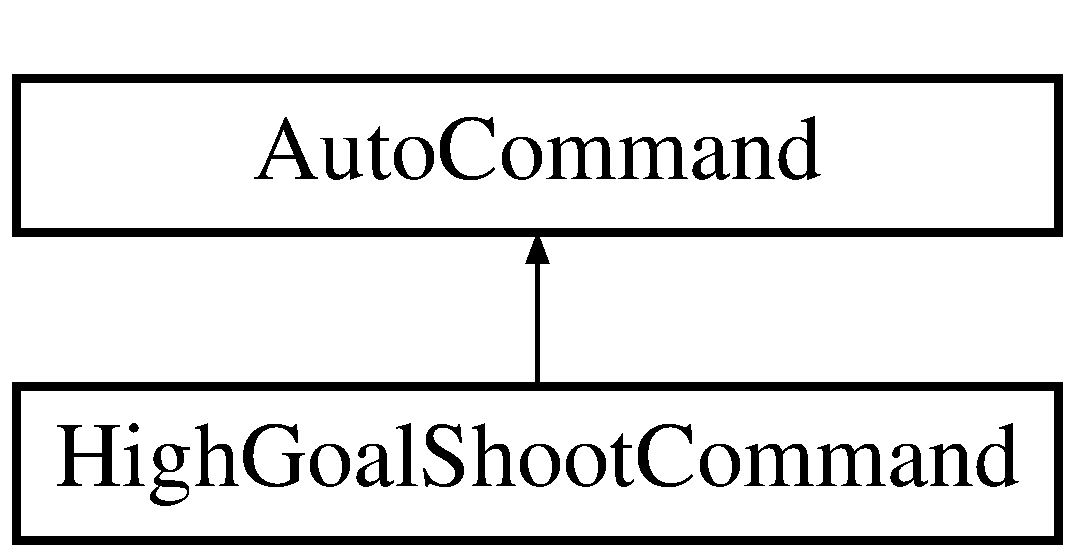
\includegraphics[height=2.000000cm]{class_high_goal_shoot_command}
\end{center}
\end{figure}
\subsection*{Public Member Functions}
\begin{DoxyCompactItemize}
\item 
\mbox{\Hypertarget{class_high_goal_shoot_command_a3e6281bd69c1ba42b2b55a8fe7a47381}\label{class_high_goal_shoot_command_a3e6281bd69c1ba42b2b55a8fe7a47381}} 
{\bfseries High\+Goal\+Shoot\+Command} (\hyperlink{class_superstructure_controller}{Superstructure\+Controller} $\ast$my\+Superstructure)
\item 
\mbox{\Hypertarget{class_high_goal_shoot_command_a8268066dc4809492290a88a5f65e277d}\label{class_high_goal_shoot_command_a8268066dc4809492290a88a5f65e277d}} 
void {\bfseries Init} ()
\item 
\mbox{\Hypertarget{class_high_goal_shoot_command_afa9e819bb0c0ae3ed8d47d67af95ed2e}\label{class_high_goal_shoot_command_afa9e819bb0c0ae3ed8d47d67af95ed2e}} 
void {\bfseries Update} (double curr\+Time\+Sec, double delta\+Time\+Sec)
\item 
\mbox{\Hypertarget{class_high_goal_shoot_command_a4a193b798e8ec374abcae6b33b974e1d}\label{class_high_goal_shoot_command_a4a193b798e8ec374abcae6b33b974e1d}} 
bool {\bfseries Is\+Done} ()
\end{DoxyCompactItemize}
\subsection*{Private Attributes}
\begin{DoxyCompactItemize}
\item 
\mbox{\Hypertarget{class_high_goal_shoot_command_ab652d73c7e2968cf1b340edf1fd3b3e1}\label{class_high_goal_shoot_command_ab652d73c7e2968cf1b340edf1fd3b3e1}} 
\hyperlink{class_superstructure_controller}{Superstructure\+Controller} $\ast$ {\bfseries superstructure\+\_\+}
\item 
\mbox{\Hypertarget{class_high_goal_shoot_command_aef45a8845bd90a878398abd5b4c8a5cb}\label{class_high_goal_shoot_command_aef45a8845bd90a878398abd5b4c8a5cb}} 
bool {\bfseries is\+Done\+\_\+}
\end{DoxyCompactItemize}


The documentation for this class was generated from the following files\+:\begin{DoxyCompactItemize}
\item 
/\+Users/maggiewang/\+Space\+\_\+\+Cookies/spacecookies/frc2017/src/\+Auto/\+Commands/High\+Goal\+Shoot\+Command.\+h\item 
/\+Users/maggiewang/\+Space\+\_\+\+Cookies/spacecookies/frc2017/src/\+Auto/\+Commands/High\+Goal\+Shoot\+Command.\+cpp\end{DoxyCompactItemize}

\hypertarget{classinstrumentation}{}\section{instrumentation Class Reference}
\label{classinstrumentation}\index{instrumentation@{instrumentation}}


{\ttfamily \#include $<$Instrumentation.\+h$>$}

\subsection*{Static Public Member Functions}
\begin{DoxyCompactItemize}
\item 
\mbox{\Hypertarget{classinstrumentation_adf9cadbff6a0bb8d6389ff79f445cd16}\label{classinstrumentation_adf9cadbff6a0bb8d6389ff79f445cd16}} 
static void {\bfseries On\+No\+Progress} ()
\item 
\mbox{\Hypertarget{classinstrumentation_ac3ba7e60a4e842298db281a3f73c9b87}\label{classinstrumentation_ac3ba7e60a4e842298db281a3f73c9b87}} 
static void {\bfseries On\+Underrun} ()
\item 
\mbox{\Hypertarget{classinstrumentation_ac2d9046a4665b5fca81f4541433f36c2}\label{classinstrumentation_ac2d9046a4665b5fca81f4541433f36c2}} 
static const char $\ast$ {\bfseries Str\+Output\+Enable} (unsigned int value)
\item 
static void \hyperlink{classinstrumentation_a0e96d2ff2bcd277f57dd1faca76c28b2}{Process} (C\+A\+N\+Talon\+::\+Motion\+Profile\+Status \&status)
\end{DoxyCompactItemize}


\subsection{Detailed Description}
Since this example focuses on Motion Control, lets print everything related to MP in a clean format. Expect to see something like......

Hold 2048 0 0 1 5.\+0 0.\+0 Hold 2048 0 0 1 5.\+0 0.\+0 output\+Enable top\+Buffer\+Rem top\+Buffer\+Cnt btm\+Buffer\+Cnt Is\+Valid Has\+Underrun Is\+Underrun Is\+Last Vel\+Only targ\+Pos targ\+Vel Hold 2048 0 0 1 5.\+0 0.\+0 Hold 2048 0 0 1 5.\+0 0.\+0 Hold 2048 0 0 1 5.\+0 0.\+0 Hold 2048 0 0 1 5.\+0 0.\+0 Hold 2048 0 0 1 5.\+0 0.\+0 Hold 2048 0 0 1 5.\+0 0.\+0 Hold 2048 0 0 1 5.\+0 0.\+0 output\+Enable top\+Buffer\+Rem top\+Buffer\+Cnt btm\+Buffer\+Cnt Is\+Valid Has\+Underrun Is\+Underrun Is\+Last Vel\+Only targ\+Pos targ\+Vel Hold 2048 0 0 1 5.\+0 0.\+0 Hold 2048 0 0 1 5.\+0 0.\+0 Hold 2048 0 0 1 5.\+0 0.\+0

...where the columns are reprinted occasionally so you know whats up. 

\subsection{Member Function Documentation}
\mbox{\Hypertarget{classinstrumentation_a0e96d2ff2bcd277f57dd1faca76c28b2}\label{classinstrumentation_a0e96d2ff2bcd277f57dd1faca76c28b2}} 
\index{instrumentation@{instrumentation}!Process@{Process}}
\index{Process@{Process}!instrumentation@{instrumentation}}
\subsubsection{\texorpdfstring{Process()}{Process()}}
{\footnotesize\ttfamily static void instrumentation\+::\+Process (\begin{DoxyParamCaption}\item[{C\+A\+N\+Talon\+::\+Motion\+Profile\+Status \&}]{status }\end{DoxyParamCaption})\hspace{0.3cm}{\ttfamily [inline]}, {\ttfamily [static]}}

Prints and/or logging to watch the MP signals 

The documentation for this class was generated from the following file\+:\begin{DoxyCompactItemize}
\item 
/\+Users/maggiewang/\+Space\+\_\+\+Cookies/spacecookies/frc2017/src/\+Auto/\+Motion\+Profiling/Instrumentation.\+h\end{DoxyCompactItemize}

\hypertarget{class_lift_one___motion_profile}{}\section{Lift\+One\+\_\+\+Motion\+Profile Class Reference}
\label{class_lift_one___motion_profile}\index{Lift\+One\+\_\+\+Motion\+Profile@{Lift\+One\+\_\+\+Motion\+Profile}}
Inheritance diagram for Lift\+One\+\_\+\+Motion\+Profile\+:\begin{figure}[H]
\begin{center}
\leavevmode
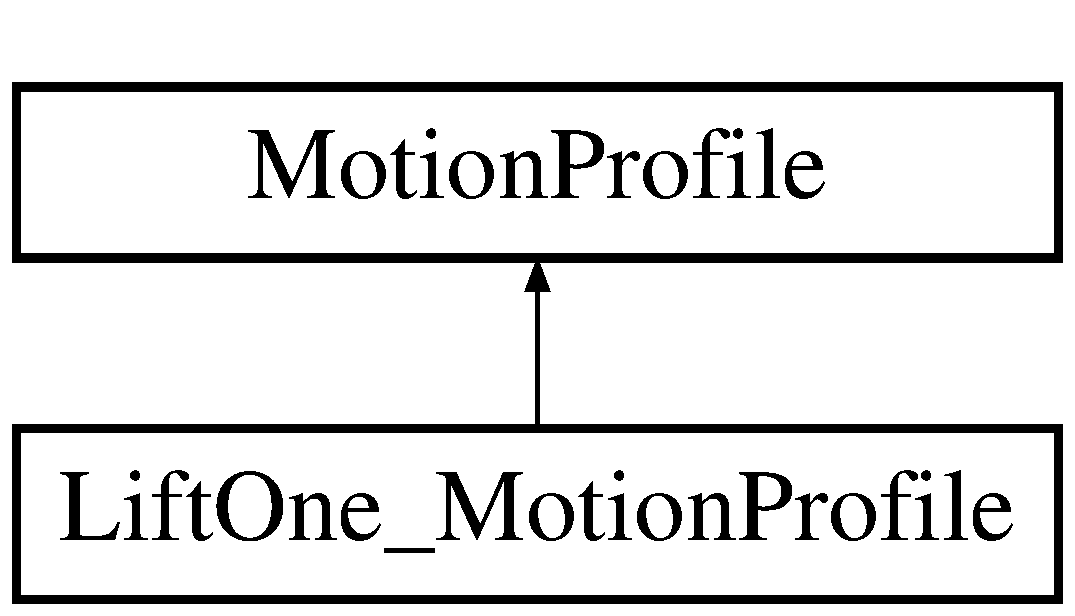
\includegraphics[height=2.000000cm]{class_lift_one___motion_profile}
\end{center}
\end{figure}
\subsection*{Public Member Functions}
\begin{DoxyCompactItemize}
\item 
\mbox{\Hypertarget{class_lift_one___motion_profile_a9600270fa65c2c590470f7852f00aa0d}\label{class_lift_one___motion_profile_a9600270fa65c2c590470f7852f00aa0d}} 
virtual int {\bfseries Get\+Length\+Of\+Left\+Motion\+Profile} ()
\item 
\mbox{\Hypertarget{class_lift_one___motion_profile_a735ae0ce072abd8f057e53292239e244}\label{class_lift_one___motion_profile_a735ae0ce072abd8f057e53292239e244}} 
virtual int {\bfseries Get\+Length\+Of\+Right\+Motion\+Profile} ()
\item 
\mbox{\Hypertarget{class_lift_one___motion_profile_a9675e08887c8d9f2937f825405da8fc9}\label{class_lift_one___motion_profile_a9675e08887c8d9f2937f825405da8fc9}} 
virtual double($\ast$ {\bfseries Get\+Left\+Motion\+Profile} ())\mbox{[}3\mbox{]}
\item 
\mbox{\Hypertarget{class_lift_one___motion_profile_a36719853fd6e5c43a007c2eb25752f60}\label{class_lift_one___motion_profile_a36719853fd6e5c43a007c2eb25752f60}} 
virtual double($\ast$ {\bfseries Get\+Right\+Motion\+Profile} ())\mbox{[}3\mbox{]}
\end{DoxyCompactItemize}
\subsection*{Private Attributes}
\begin{DoxyCompactItemize}
\item 
\mbox{\Hypertarget{class_lift_one___motion_profile_ad31c1278f6fcf90e77f1754e1bde2c08}\label{class_lift_one___motion_profile_ad31c1278f6fcf90e77f1754e1bde2c08}} 
int {\bfseries k\+Left\+Motion\+Profile\+Sz} = 214
\item 
\mbox{\Hypertarget{class_lift_one___motion_profile_a5822b92a9beeb75b3c07b0ce256f3c06}\label{class_lift_one___motion_profile_a5822b92a9beeb75b3c07b0ce256f3c06}} 
double {\bfseries k\+Left\+Motion\+Profile} \mbox{[}214\mbox{]}\mbox{[}3\mbox{]}
\item 
\mbox{\Hypertarget{class_lift_one___motion_profile_ad6c248f6020e78a0c47089316883a045}\label{class_lift_one___motion_profile_ad6c248f6020e78a0c47089316883a045}} 
int {\bfseries k\+Right\+Motion\+Profile\+Sz} = 214
\item 
\mbox{\Hypertarget{class_lift_one___motion_profile_af47a55f1855f2bcac92b8fc0ba0c1a90}\label{class_lift_one___motion_profile_af47a55f1855f2bcac92b8fc0ba0c1a90}} 
double {\bfseries k\+Right\+Motion\+Profile} \mbox{[}214\mbox{]}\mbox{[}3\mbox{]}
\end{DoxyCompactItemize}
\subsection*{Additional Inherited Members}


The documentation for this class was generated from the following file\+:\begin{DoxyCompactItemize}
\item 
/\+Users/maggiewang/\+Space\+\_\+\+Cookies/spacecookies/frc2017/src/\+Auto/\+Motion\+Profiling/Lift\+One\+\_\+\+Motion\+Profile.\+h\end{DoxyCompactItemize}

\hypertarget{class_lift_three___motion_profile}{}\section{Lift\+Three\+\_\+\+Motion\+Profile Class Reference}
\label{class_lift_three___motion_profile}\index{Lift\+Three\+\_\+\+Motion\+Profile@{Lift\+Three\+\_\+\+Motion\+Profile}}
Inheritance diagram for Lift\+Three\+\_\+\+Motion\+Profile\+:\begin{figure}[H]
\begin{center}
\leavevmode
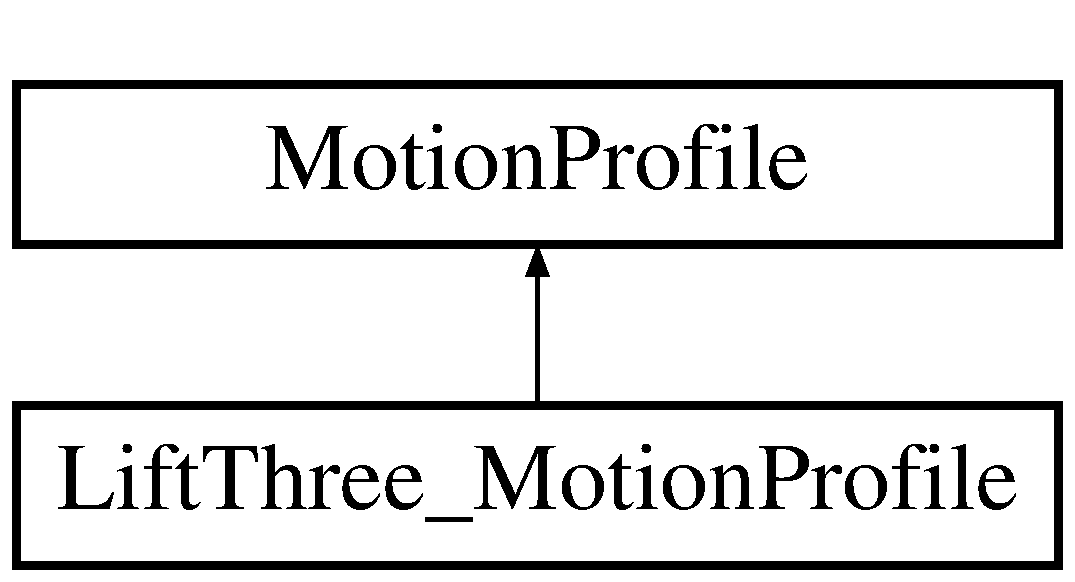
\includegraphics[height=2.000000cm]{class_lift_three___motion_profile}
\end{center}
\end{figure}
\subsection*{Public Member Functions}
\begin{DoxyCompactItemize}
\item 
\mbox{\Hypertarget{class_lift_three___motion_profile_a0fd9d60707d0479290a168a4686cd22a}\label{class_lift_three___motion_profile_a0fd9d60707d0479290a168a4686cd22a}} 
virtual int {\bfseries Get\+Length\+Of\+Left\+Motion\+Profile} ()
\item 
\mbox{\Hypertarget{class_lift_three___motion_profile_ae3ee694eef88dab61c48a5e32e09657d}\label{class_lift_three___motion_profile_ae3ee694eef88dab61c48a5e32e09657d}} 
virtual int {\bfseries Get\+Length\+Of\+Right\+Motion\+Profile} ()
\item 
\mbox{\Hypertarget{class_lift_three___motion_profile_a8697de71677b1ce2aaf06c7220d8f6aa}\label{class_lift_three___motion_profile_a8697de71677b1ce2aaf06c7220d8f6aa}} 
virtual double($\ast$ {\bfseries Get\+Left\+Motion\+Profile} ())\mbox{[}3\mbox{]}
\item 
\mbox{\Hypertarget{class_lift_three___motion_profile_ac08df00ab2c8cce31ba6aa5189d2c05a}\label{class_lift_three___motion_profile_ac08df00ab2c8cce31ba6aa5189d2c05a}} 
virtual double($\ast$ {\bfseries Get\+Right\+Motion\+Profile} ())\mbox{[}3\mbox{]}
\end{DoxyCompactItemize}
\subsection*{Private Attributes}
\begin{DoxyCompactItemize}
\item 
\mbox{\Hypertarget{class_lift_three___motion_profile_a90da7fce23a181a414d31f9e1bea66ce}\label{class_lift_three___motion_profile_a90da7fce23a181a414d31f9e1bea66ce}} 
int {\bfseries k\+Left\+Motion\+Profile\+Sz} = 214
\item 
\mbox{\Hypertarget{class_lift_three___motion_profile_ae3bd28d6ba1f1364bfa85225afa4c944}\label{class_lift_three___motion_profile_ae3bd28d6ba1f1364bfa85225afa4c944}} 
double {\bfseries k\+Left\+Motion\+Profile} \mbox{[}214\mbox{]}\mbox{[}3\mbox{]}
\item 
\mbox{\Hypertarget{class_lift_three___motion_profile_a755630b6159be136796a97a2fac1fbd3}\label{class_lift_three___motion_profile_a755630b6159be136796a97a2fac1fbd3}} 
int {\bfseries k\+Right\+Motion\+Profile\+Sz} = 214
\item 
\mbox{\Hypertarget{class_lift_three___motion_profile_a67072de36b4ee7ea11c988b58f69ce49}\label{class_lift_three___motion_profile_a67072de36b4ee7ea11c988b58f69ce49}} 
double {\bfseries k\+Right\+Motion\+Profile} \mbox{[}214\mbox{]}\mbox{[}3\mbox{]}
\end{DoxyCompactItemize}
\subsection*{Additional Inherited Members}


The documentation for this class was generated from the following file\+:\begin{DoxyCompactItemize}
\item 
/\+Users/maggiewang/\+Space\+\_\+\+Cookies/spacecookies/frc2017/src/\+Auto/\+Motion\+Profiling/Lift\+Three\+\_\+\+Motion\+Profile.\+h\end{DoxyCompactItemize}

\hypertarget{class_lift_two___motion_profile}{}\section{Lift\+Two\+\_\+\+Motion\+Profile Class Reference}
\label{class_lift_two___motion_profile}\index{Lift\+Two\+\_\+\+Motion\+Profile@{Lift\+Two\+\_\+\+Motion\+Profile}}
Inheritance diagram for Lift\+Two\+\_\+\+Motion\+Profile\+:\begin{figure}[H]
\begin{center}
\leavevmode
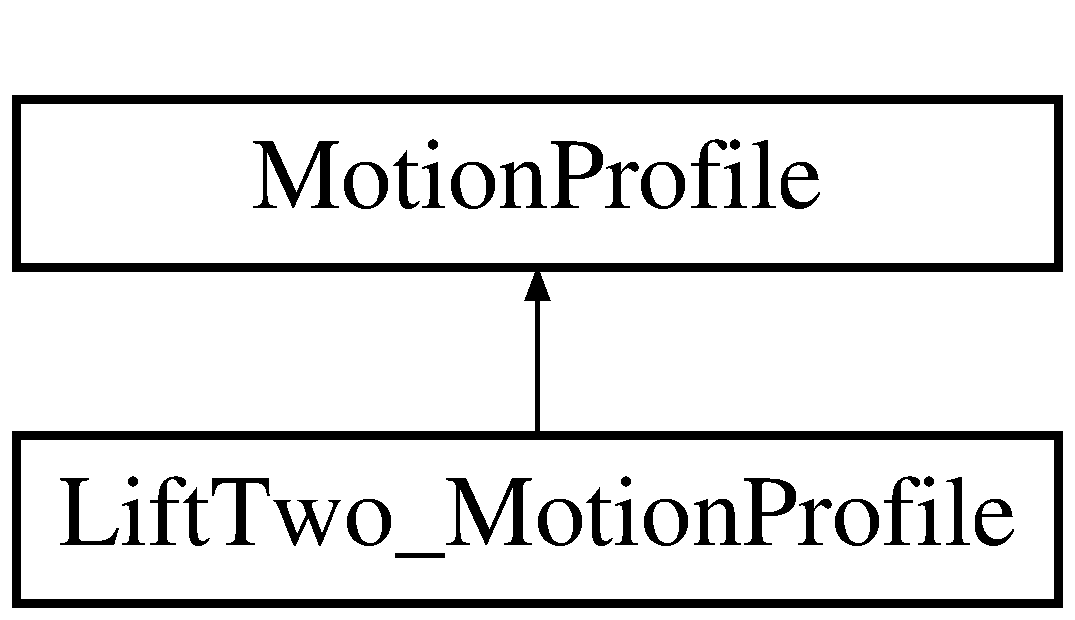
\includegraphics[height=2.000000cm]{class_lift_two___motion_profile}
\end{center}
\end{figure}
\subsection*{Public Member Functions}
\begin{DoxyCompactItemize}
\item 
\mbox{\Hypertarget{class_lift_two___motion_profile_a4d35a32fe4f2fa5680b524997f8a4bb3}\label{class_lift_two___motion_profile_a4d35a32fe4f2fa5680b524997f8a4bb3}} 
virtual int {\bfseries Get\+Length\+Of\+Left\+Motion\+Profile} ()
\item 
\mbox{\Hypertarget{class_lift_two___motion_profile_af7766868c73229c5697ab43fe7b54332}\label{class_lift_two___motion_profile_af7766868c73229c5697ab43fe7b54332}} 
virtual int {\bfseries Get\+Length\+Of\+Right\+Motion\+Profile} ()
\item 
\mbox{\Hypertarget{class_lift_two___motion_profile_a28ca86c6fe0f9221f3fb5c8712f048e9}\label{class_lift_two___motion_profile_a28ca86c6fe0f9221f3fb5c8712f048e9}} 
virtual double($\ast$ {\bfseries Get\+Left\+Motion\+Profile} ())\mbox{[}3\mbox{]}
\item 
\mbox{\Hypertarget{class_lift_two___motion_profile_a7d2ccce0ea921859c1954e16a78244e0}\label{class_lift_two___motion_profile_a7d2ccce0ea921859c1954e16a78244e0}} 
virtual double($\ast$ {\bfseries Get\+Right\+Motion\+Profile} ())\mbox{[}3\mbox{]}
\end{DoxyCompactItemize}
\subsection*{Private Attributes}
\begin{DoxyCompactItemize}
\item 
\mbox{\Hypertarget{class_lift_two___motion_profile_a0879ecc00fb19e24b88dbf98265620be}\label{class_lift_two___motion_profile_a0879ecc00fb19e24b88dbf98265620be}} 
int {\bfseries k\+Left\+Motion\+Profile\+Sz} = 204
\item 
\mbox{\Hypertarget{class_lift_two___motion_profile_afdf0a9aa9b87457b77d5310c6c7a8ad6}\label{class_lift_two___motion_profile_afdf0a9aa9b87457b77d5310c6c7a8ad6}} 
double {\bfseries k\+Left\+Motion\+Profile} \mbox{[}204\mbox{]}\mbox{[}3\mbox{]}
\item 
\mbox{\Hypertarget{class_lift_two___motion_profile_ac64febf8116e7553bf61639f50b14429}\label{class_lift_two___motion_profile_ac64febf8116e7553bf61639f50b14429}} 
int {\bfseries k\+Right\+Motion\+Profile\+Sz} = 204
\item 
\mbox{\Hypertarget{class_lift_two___motion_profile_a8642c60479303174610b4dc72d734126}\label{class_lift_two___motion_profile_a8642c60479303174610b4dc72d734126}} 
double {\bfseries k\+Right\+Motion\+Profile} \mbox{[}204\mbox{]}\mbox{[}3\mbox{]}
\end{DoxyCompactItemize}
\subsection*{Additional Inherited Members}


The documentation for this class was generated from the following file\+:\begin{DoxyCompactItemize}
\item 
/\+Users/maggiewang/\+Space\+\_\+\+Cookies/spacecookies/frc2017/src/\+Auto/\+Motion\+Profiling/Lift\+Two\+\_\+\+Motion\+Profile.\+h\end{DoxyCompactItemize}

\hypertarget{class_main_program}{}\section{Main\+Program Class Reference}
\label{class_main_program}\index{Main\+Program@{Main\+Program}}
Inheritance diagram for Main\+Program\+:\begin{figure}[H]
\begin{center}
\leavevmode
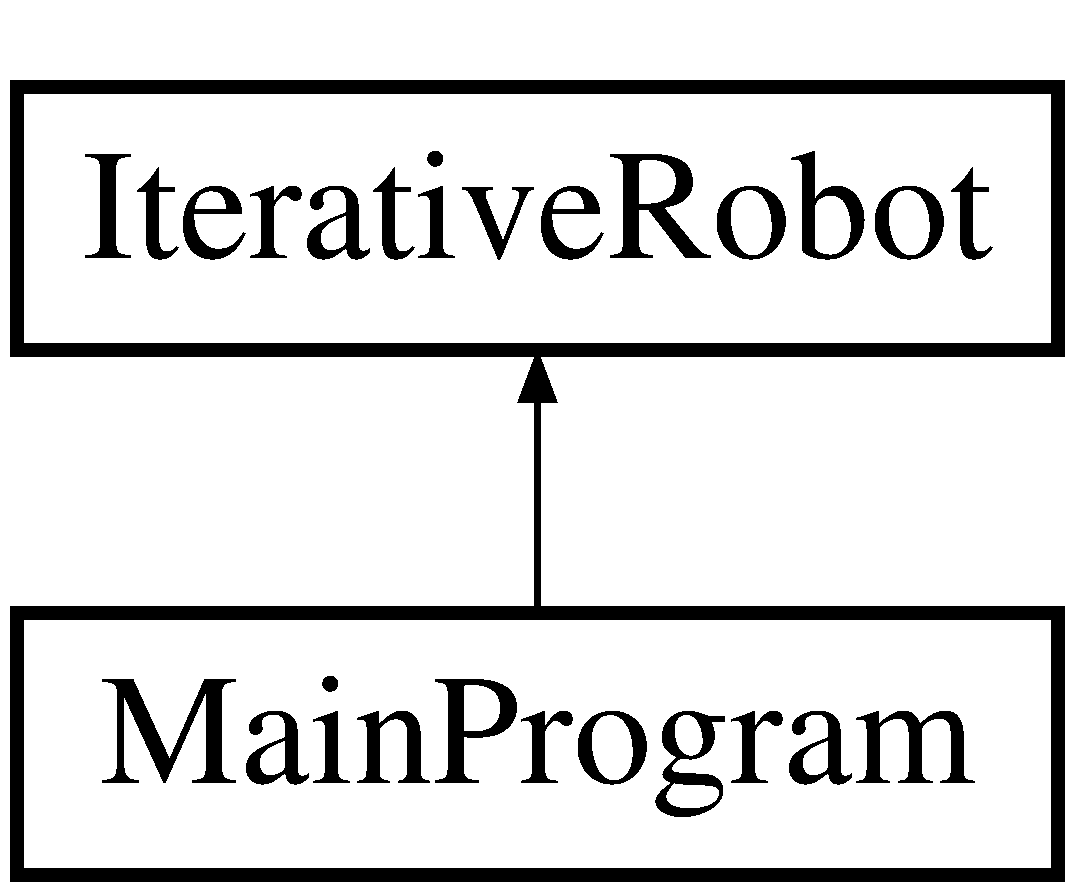
\includegraphics[height=2.000000cm]{class_main_program}
\end{center}
\end{figure}
\subsection*{Public Member Functions}
\begin{DoxyCompactItemize}
\item 
\mbox{\Hypertarget{class_main_program_a7e874801d13eddebc3d6abb0bddcd741}\label{class_main_program_a7e874801d13eddebc3d6abb0bddcd741}} 
void {\bfseries Robot\+Init} ()
\item 
\mbox{\Hypertarget{class_main_program_a0e4b90779d59d7d37534514a7f53e70d}\label{class_main_program_a0e4b90779d59d7d37534514a7f53e70d}} 
void {\bfseries Autonomous\+Init} ()
\item 
\mbox{\Hypertarget{class_main_program_a203b4b5345da0064b1131be9e769ce44}\label{class_main_program_a203b4b5345da0064b1131be9e769ce44}} 
void {\bfseries Autonomous\+Periodic} ()
\item 
\mbox{\Hypertarget{class_main_program_a7c27fa2f63d0289ec779ca2d8cf17db7}\label{class_main_program_a7c27fa2f63d0289ec779ca2d8cf17db7}} 
void {\bfseries Teleop\+Init} ()
\item 
\mbox{\Hypertarget{class_main_program_a9ad6dd3b0af4928522a2f51f93a502ab}\label{class_main_program_a9ad6dd3b0af4928522a2f51f93a502ab}} 
void {\bfseries Teleop\+Periodic} ()
\item 
\mbox{\Hypertarget{class_main_program_a6cc3d4d9df4c41a2c0d69338d7a232a8}\label{class_main_program_a6cc3d4d9df4c41a2c0d69338d7a232a8}} 
void {\bfseries Test\+Init} ()
\item 
\mbox{\Hypertarget{class_main_program_ae39fe132e153d724c9b0991e5c8b72ea}\label{class_main_program_ae39fe132e153d724c9b0991e5c8b72ea}} 
void {\bfseries Test\+Periodic} ()
\end{DoxyCompactItemize}
\subsection*{Private Member Functions}
\begin{DoxyCompactItemize}
\item 
\mbox{\Hypertarget{class_main_program_a14bb707e4f84a60a734be54aac0cda79}\label{class_main_program_a14bb707e4f84a60a734be54aac0cda79}} 
void {\bfseries Reset\+Timer\+Variables} ()
\item 
\mbox{\Hypertarget{class_main_program_a28c1b51061cfbe7bbe37cd7857408d0b}\label{class_main_program_a28c1b51061cfbe7bbe37cd7857408d0b}} 
void {\bfseries Update\+Timer\+Variables} ()
\item 
\mbox{\Hypertarget{class_main_program_aa696c8af3e8a78a702c6d18f0f7af3ea}\label{class_main_program_aa696c8af3e8a78a702c6d18f0f7af3ea}} 
void {\bfseries Reset\+Controllers} ()
\end{DoxyCompactItemize}
\subsection*{Private Attributes}
\begin{DoxyCompactItemize}
\item 
\hyperlink{class_robot_model}{Robot\+Model} $\ast$ \hyperlink{class_main_program_a2d74d25ebc0a0bc52daa34a0048e071d}{robot\+\_\+}
\item 
\mbox{\Hypertarget{class_main_program_a8b0df9956703e91662bef87dbe6552c6}\label{class_main_program_a8b0df9956703e91662bef87dbe6552c6}} 
\hyperlink{class_control_board}{Control\+Board} $\ast$ {\bfseries human\+Control\+\_\+}
\item 
\mbox{\Hypertarget{class_main_program_ad4224352ece515213597c083c02d89bc}\label{class_main_program_ad4224352ece515213597c083c02d89bc}} 
\hyperlink{class_drive_controller}{Drive\+Controller} $\ast$ {\bfseries drive\+Controller\+\_\+}
\item 
\mbox{\Hypertarget{class_main_program_a0dfd4823ff497148a70f22b0dfccd230}\label{class_main_program_a0dfd4823ff497148a70f22b0dfccd230}} 
\hyperlink{class_superstructure_controller}{Superstructure\+Controller} $\ast$ {\bfseries superstructure\+Controller\+\_\+}
\item 
\mbox{\Hypertarget{class_main_program_ac3d5377aaf3e901441354f9c9d641453}\label{class_main_program_ac3d5377aaf3e901441354f9c9d641453}} 
\hyperlink{class_auto_controller}{Auto\+Controller} $\ast$ {\bfseries auto\+Controller\+\_\+}
\item 
\mbox{\Hypertarget{class_main_program_abe37903ef51d2df9dc89f69a32e8da67}\label{class_main_program_abe37903ef51d2df9dc89f69a32e8da67}} 
Live\+Window $\ast$ {\bfseries live\+Window\+\_\+}
\item 
\mbox{\Hypertarget{class_main_program_a3787d55d75893503e7f33f441676d193}\label{class_main_program_a3787d55d75893503e7f33f441676d193}} 
\hyperlink{class_one_gear_mode}{One\+Gear\+Mode} $\ast$ {\bfseries lift\+Mode\+\_\+}
\item 
\mbox{\Hypertarget{class_main_program_a180a107906b59bbdadce0a366a952da5}\label{class_main_program_a180a107906b59bbdadce0a366a952da5}} 
double {\bfseries curr\+Time\+Sec\+\_\+}
\item 
\mbox{\Hypertarget{class_main_program_a6c22d1b8be27e874668c2cb240f0aaa8}\label{class_main_program_a6c22d1b8be27e874668c2cb240f0aaa8}} 
double {\bfseries last\+Time\+Sec\+\_\+}
\item 
\mbox{\Hypertarget{class_main_program_a3259650f3390bc05a34f9ca2b58bc5bb}\label{class_main_program_a3259650f3390bc05a34f9ca2b58bc5bb}} 
double {\bfseries delta\+Time\+Sec\+\_\+}
\end{DoxyCompactItemize}


\subsection{Member Data Documentation}
\mbox{\Hypertarget{class_main_program_a2d74d25ebc0a0bc52daa34a0048e071d}\label{class_main_program_a2d74d25ebc0a0bc52daa34a0048e071d}} 
\index{Main\+Program@{Main\+Program}!robot\+\_\+@{robot\+\_\+}}
\index{robot\+\_\+@{robot\+\_\+}!Main\+Program@{Main\+Program}}
\subsubsection{\texorpdfstring{robot\+\_\+}{robot\_}}
{\footnotesize\ttfamily \hyperlink{class_robot_model}{Robot\+Model}$\ast$ Main\+Program\+::robot\+\_\+\hspace{0.3cm}{\ttfamily [private]}}

Testing. 

The documentation for this class was generated from the following file\+:\begin{DoxyCompactItemize}
\item 
/\+Users/maggiewang/\+Space\+\_\+\+Cookies/spacecookies/frc2017/src/Main\+Program.\+cpp\end{DoxyCompactItemize}

\hypertarget{class_motion_profile}{}\section{Motion\+Profile Class Reference}
\label{class_motion_profile}\index{Motion\+Profile@{Motion\+Profile}}
Inheritance diagram for Motion\+Profile\+:\begin{figure}[H]
\begin{center}
\leavevmode
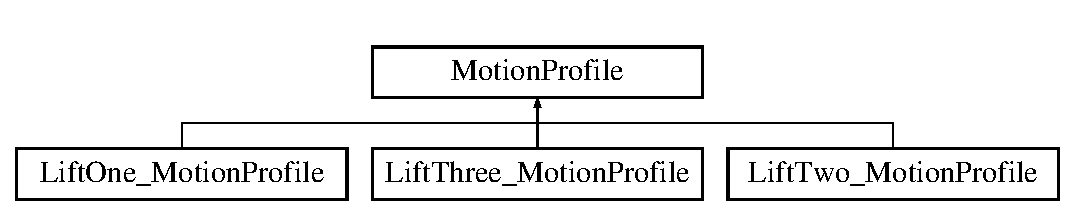
\includegraphics[height=2.000000cm]{class_motion_profile}
\end{center}
\end{figure}
\subsection*{Public Member Functions}
\begin{DoxyCompactItemize}
\item 
\mbox{\Hypertarget{class_motion_profile_a9639c4bb07b29bd3aa95023164387ee4}\label{class_motion_profile_a9639c4bb07b29bd3aa95023164387ee4}} 
virtual int {\bfseries Get\+Length\+Of\+Left\+Motion\+Profile} ()
\item 
\mbox{\Hypertarget{class_motion_profile_ac7e7b2097e4b4f12b4d065db530f26d2}\label{class_motion_profile_ac7e7b2097e4b4f12b4d065db530f26d2}} 
virtual int {\bfseries Get\+Length\+Of\+Right\+Motion\+Profile} ()
\item 
\mbox{\Hypertarget{class_motion_profile_a7758fb7971a13c098b019a5f05bf6dda}\label{class_motion_profile_a7758fb7971a13c098b019a5f05bf6dda}} 
virtual double($\ast$ {\bfseries Get\+Left\+Motion\+Profile} ())\mbox{[}3\mbox{]}
\item 
\mbox{\Hypertarget{class_motion_profile_a9260edbeabd693944002363dbe337bed}\label{class_motion_profile_a9260edbeabd693944002363dbe337bed}} 
virtual double($\ast$ {\bfseries Get\+Right\+Motion\+Profile} ())\mbox{[}3\mbox{]}
\end{DoxyCompactItemize}
\subsection*{Public Attributes}
\begin{DoxyCompactItemize}
\item 
\mbox{\Hypertarget{class_motion_profile_a4b8366ff0f33d91d9a427bd93b7ceb69}\label{class_motion_profile_a4b8366ff0f33d91d9a427bd93b7ceb69}} 
int {\bfseries k\+Left\+Motion\+Profile\+Sz} = 0
\item 
\mbox{\Hypertarget{class_motion_profile_a9c911a0a62025c5541d85e066666dd4c}\label{class_motion_profile_a9c911a0a62025c5541d85e066666dd4c}} 
double {\bfseries k\+Left\+Motion\+Profile} \mbox{[}$\,$\mbox{]}\mbox{[}3\mbox{]}
\item 
\mbox{\Hypertarget{class_motion_profile_a73adb65b3ef772ab29d21774f572044b}\label{class_motion_profile_a73adb65b3ef772ab29d21774f572044b}} 
int {\bfseries k\+Right\+Motion\+Profile\+Sz} = 0
\item 
\mbox{\Hypertarget{class_motion_profile_ad5cd0bbcee9e5b9bf77610142df879c5}\label{class_motion_profile_ad5cd0bbcee9e5b9bf77610142df879c5}} 
double {\bfseries k\+Right\+Motion\+Profile} \mbox{[}$\,$\mbox{]}\mbox{[}3\mbox{]}
\end{DoxyCompactItemize}


The documentation for this class was generated from the following file\+:\begin{DoxyCompactItemize}
\item 
/\+Users/maggiewang/\+Space\+\_\+\+Cookies/spacecookies/frc2017/src/\+Auto/\+Motion\+Profiling/Motion\+Profile.\+h\end{DoxyCompactItemize}

\hypertarget{class_motion_profile_executor}{}\section{Motion\+Profile\+Executor Class Reference}
\label{class_motion_profile_executor}\index{Motion\+Profile\+Executor@{Motion\+Profile\+Executor}}


{\ttfamily \#include $<$Motion\+Profile\+Executor.\+h$>$}

\subsection*{Public Member Functions}
\begin{DoxyCompactItemize}
\item 
void \hyperlink{class_motion_profile_executor_a6599521948ebfd609d9b4c53539f597f}{Periodic\+Task} ()
\item 
\mbox{\Hypertarget{class_motion_profile_executor_aa552856d9f744a9a38add555eac3669b}\label{class_motion_profile_executor_aa552856d9f744a9a38add555eac3669b}} 
{\bfseries Motion\+Profile\+Executor} (C\+A\+N\+Talon \&talon, double profile\mbox{[}$\,$\mbox{]}\mbox{[}3\mbox{]}, int traj\+Length)
\item 
void \hyperlink{class_motion_profile_executor_a3e94905fe37d30840822bd819978b79d}{reset} ()
\item 
void \hyperlink{class_motion_profile_executor_a60a8d4ab5b168b31e75619b2a3683a78}{control} ()
\item 
void \hyperlink{class_motion_profile_executor_a16ef527ec6fea68ae7ac06785ddb3b7c}{start\+Filling} ()
\item 
\mbox{\Hypertarget{class_motion_profile_executor_a1a77e57ff634e1189fe3fe2249bbff3b}\label{class_motion_profile_executor_a1a77e57ff634e1189fe3fe2249bbff3b}} 
void {\bfseries start\+Filling} (double $\ast$$\ast$profile, int total\+Cnt)
\item 
void \hyperlink{class_motion_profile_executor_a49d7debb97c9c722ee8fc2f6d43d21ca}{start} ()
\item 
C\+A\+N\+Talon\+::\+Set\+Value\+Motion\+Profile \hyperlink{class_motion_profile_executor_aad1297807d386b66246ca4154e136485}{get\+Set\+Value} ()
\end{DoxyCompactItemize}
\subsection*{Public Attributes}
\begin{DoxyCompactItemize}
\item 
C\+A\+N\+Talon\+::\+Motion\+Profile\+Status \hyperlink{class_motion_profile_executor_ab99b425d2adf9904079634fd61e10b96}{status\+\_\+}
\item 
C\+A\+N\+Talon \& \hyperlink{class_motion_profile_executor_af9d5579de49093673fac4e35819e7e0f}{talon\+\_\+}
\item 
int \hyperlink{class_motion_profile_executor_af971a9eb8807ea12c7d70befe44d2122}{state\+\_\+} = 0
\item 
int \hyperlink{class_motion_profile_executor_aba6cb888640b9bb7c169e1bf33de92b3}{loop\+Timeout\+\_\+} = -\/1
\item 
bool \hyperlink{class_motion_profile_executor_a60632854bbae77815fbafa3b8c1450e7}{b\+Start\+\_\+} = false
\item 
\mbox{\Hypertarget{class_motion_profile_executor_aef583c74fa3c313e758b5f3c1b48ae53}\label{class_motion_profile_executor_aef583c74fa3c313e758b5f3c1b48ae53}} 
bool {\bfseries is\+Left\+\_\+} = false
\item 
\mbox{\Hypertarget{class_motion_profile_executor_ade8df55aeb5c88635782f7e2ccf473ca}\label{class_motion_profile_executor_ade8df55aeb5c88635782f7e2ccf473ca}} 
bool {\bfseries has\+Started\+\_\+} = false
\item 
\mbox{\Hypertarget{class_motion_profile_executor_ae973dbde77522dae4166e039fb3f646e}\label{class_motion_profile_executor_ae973dbde77522dae4166e039fb3f646e}} 
bool {\bfseries is\+Done\+\_\+} = false
\item 
\mbox{\Hypertarget{class_motion_profile_executor_a46c706826d1b78146e340947696e5232}\label{class_motion_profile_executor_a46c706826d1b78146e340947696e5232}} 
double $\ast$$\ast$ {\bfseries profile\+\_\+}
\item 
\mbox{\Hypertarget{class_motion_profile_executor_a05e5a41867c021b9ff7c9f7c72ad5d46}\label{class_motion_profile_executor_a05e5a41867c021b9ff7c9f7c72ad5d46}} 
int {\bfseries traj\+Length\+\_\+}
\item 
C\+A\+N\+Talon\+::\+Set\+Value\+Motion\+Profile \hyperlink{class_motion_profile_executor_a34d9e17b3cdf0ad0a117cc2cc995e85f}{set\+Value\+\_\+} = C\+A\+N\+Talon\+::\+Set\+Value\+Motion\+Profile\+Disable
\item 
Notifier \hyperlink{class_motion_profile_executor_a01ac4918310bd4207fa361ee66124602}{notifer\+\_\+}
\end{DoxyCompactItemize}
\subsection*{Static Public Attributes}
\begin{DoxyCompactItemize}
\item 
static const int \hyperlink{class_motion_profile_executor_ab2cd2c282d2c57e61847f3b0baaf6663}{k\+Min\+Points\+In\+Talon} = 5
\item 
static const int \hyperlink{class_motion_profile_executor_a125cf2e048a603624b5d74691a9805ff}{k\+Num\+Loops\+Timeout} = 10
\end{DoxyCompactItemize}


\subsection{Detailed Description}
Example logic for firing and managing motion profiles. This example sends M\+Ps, waits for them to finish Although this code uses a C\+A\+N\+Talon, nowhere in this module do we change\+Mode() or call set() to change the output. This is done in Robot.\+java to demonstrate how to change control modes on the fly.

The only routines we call on Talon are....

change\+Motion\+Control\+Frame\+Period

get\+Motion\+Profile\+Status clear\+Motion\+Profile\+Has\+Underrun to get status and potentially clear the error flag.

push\+Motion\+Profile\+Trajectory clear\+Motion\+Profile\+Trajectories process\+Motion\+Profile\+Buffer, to push/clear, and process the trajectory points.

get\+Control\+Mode, to check if we are in Motion Profile Control mode.

Example of advanced features not demonstrated here... \mbox{[}1\mbox{]} Calling push\+Motion\+Profile\+Trajectory() continuously while the Talon executes the motion profile, thereby keeping it going indefinitely. \mbox{[}2\mbox{]} Instead of setting the sensor position to zero at the start of each MP, the program could offset the MP\textquotesingle{}s position based on current position. 

\subsection{Member Function Documentation}
\mbox{\Hypertarget{class_motion_profile_executor_a60a8d4ab5b168b31e75619b2a3683a78}\label{class_motion_profile_executor_a60a8d4ab5b168b31e75619b2a3683a78}} 
\index{Motion\+Profile\+Executor@{Motion\+Profile\+Executor}!control@{control}}
\index{control@{control}!Motion\+Profile\+Executor@{Motion\+Profile\+Executor}}
\subsubsection{\texorpdfstring{control()}{control()}}
{\footnotesize\ttfamily void Motion\+Profile\+Executor\+::control (\begin{DoxyParamCaption}{ }\end{DoxyParamCaption})\hspace{0.3cm}{\ttfamily [inline]}}

Called every loop. \mbox{\Hypertarget{class_motion_profile_executor_aad1297807d386b66246ca4154e136485}\label{class_motion_profile_executor_aad1297807d386b66246ca4154e136485}} 
\index{Motion\+Profile\+Executor@{Motion\+Profile\+Executor}!get\+Set\+Value@{get\+Set\+Value}}
\index{get\+Set\+Value@{get\+Set\+Value}!Motion\+Profile\+Executor@{Motion\+Profile\+Executor}}
\subsubsection{\texorpdfstring{get\+Set\+Value()}{getSetValue()}}
{\footnotesize\ttfamily C\+A\+N\+Talon\+::\+Set\+Value\+Motion\+Profile Motion\+Profile\+Executor\+::get\+Set\+Value (\begin{DoxyParamCaption}{ }\end{DoxyParamCaption})\hspace{0.3cm}{\ttfamily [inline]}}

\begin{DoxyReturn}{Returns}
the output value to pass to Talon\textquotesingle{}s set() routine. 0 for disable motion-\/profile output, 1 for enable motion-\/profile, 2 for hold current motion profile trajectory point. 
\end{DoxyReturn}
\mbox{\Hypertarget{class_motion_profile_executor_a6599521948ebfd609d9b4c53539f597f}\label{class_motion_profile_executor_a6599521948ebfd609d9b4c53539f597f}} 
\index{Motion\+Profile\+Executor@{Motion\+Profile\+Executor}!Periodic\+Task@{Periodic\+Task}}
\index{Periodic\+Task@{Periodic\+Task}!Motion\+Profile\+Executor@{Motion\+Profile\+Executor}}
\subsubsection{\texorpdfstring{Periodic\+Task()}{PeriodicTask()}}
{\footnotesize\ttfamily void Motion\+Profile\+Executor\+::\+Periodic\+Task (\begin{DoxyParamCaption}{ }\end{DoxyParamCaption})\hspace{0.3cm}{\ttfamily [inline]}}

Lets create a periodic task to funnel our trajectory points into our talon. It doesn\textquotesingle{}t need to be very accurate, just needs to keep pace with the motion profiler executer. Now if you\textquotesingle{}re trajectory points are slow, there is no need to do this, just call \+\_\+talon.\+process\+Motion\+Profile\+Buffer() in your teleop loop. Generally speaking you want to call it at least twice as fast as the duration of your trajectory points. So if they are firing every 20ms, you should call every 10ms. \mbox{\Hypertarget{class_motion_profile_executor_a3e94905fe37d30840822bd819978b79d}\label{class_motion_profile_executor_a3e94905fe37d30840822bd819978b79d}} 
\index{Motion\+Profile\+Executor@{Motion\+Profile\+Executor}!reset@{reset}}
\index{reset@{reset}!Motion\+Profile\+Executor@{Motion\+Profile\+Executor}}
\subsubsection{\texorpdfstring{reset()}{reset()}}
{\footnotesize\ttfamily void Motion\+Profile\+Executor\+::reset (\begin{DoxyParamCaption}{ }\end{DoxyParamCaption})\hspace{0.3cm}{\ttfamily [inline]}}

Called to clear Motion profile buffer and reset state info during disabled and when Talon is not in MP control mode. \mbox{\Hypertarget{class_motion_profile_executor_a49d7debb97c9c722ee8fc2f6d43d21ca}\label{class_motion_profile_executor_a49d7debb97c9c722ee8fc2f6d43d21ca}} 
\index{Motion\+Profile\+Executor@{Motion\+Profile\+Executor}!start@{start}}
\index{start@{start}!Motion\+Profile\+Executor@{Motion\+Profile\+Executor}}
\subsubsection{\texorpdfstring{start()}{start()}}
{\footnotesize\ttfamily void Motion\+Profile\+Executor\+::start (\begin{DoxyParamCaption}{ }\end{DoxyParamCaption})\hspace{0.3cm}{\ttfamily [inline]}}

Called by application to signal Talon to start the buffered MP (when it\textquotesingle{}s able to). \mbox{\Hypertarget{class_motion_profile_executor_a16ef527ec6fea68ae7ac06785ddb3b7c}\label{class_motion_profile_executor_a16ef527ec6fea68ae7ac06785ddb3b7c}} 
\index{Motion\+Profile\+Executor@{Motion\+Profile\+Executor}!start\+Filling@{start\+Filling}}
\index{start\+Filling@{start\+Filling}!Motion\+Profile\+Executor@{Motion\+Profile\+Executor}}
\subsubsection{\texorpdfstring{start\+Filling()}{startFilling()}}
{\footnotesize\ttfamily void Motion\+Profile\+Executor\+::start\+Filling (\begin{DoxyParamCaption}{ }\end{DoxyParamCaption})\hspace{0.3cm}{\ttfamily [inline]}}

Start filling the M\+Ps to all of the involved Talons. 

\subsection{Member Data Documentation}
\mbox{\Hypertarget{class_motion_profile_executor_a60632854bbae77815fbafa3b8c1450e7}\label{class_motion_profile_executor_a60632854bbae77815fbafa3b8c1450e7}} 
\index{Motion\+Profile\+Executor@{Motion\+Profile\+Executor}!b\+Start\+\_\+@{b\+Start\+\_\+}}
\index{b\+Start\+\_\+@{b\+Start\+\_\+}!Motion\+Profile\+Executor@{Motion\+Profile\+Executor}}
\subsubsection{\texorpdfstring{b\+Start\+\_\+}{bStart\_}}
{\footnotesize\ttfamily bool Motion\+Profile\+Executor\+::b\+Start\+\_\+ = false}

If \hyperlink{class_motion_profile_executor_a49d7debb97c9c722ee8fc2f6d43d21ca}{start()} gets called, this flag is set and in the \hyperlink{class_motion_profile_executor_a60a8d4ab5b168b31e75619b2a3683a78}{control()} we will service it. \mbox{\Hypertarget{class_motion_profile_executor_ab2cd2c282d2c57e61847f3b0baaf6663}\label{class_motion_profile_executor_ab2cd2c282d2c57e61847f3b0baaf6663}} 
\index{Motion\+Profile\+Executor@{Motion\+Profile\+Executor}!k\+Min\+Points\+In\+Talon@{k\+Min\+Points\+In\+Talon}}
\index{k\+Min\+Points\+In\+Talon@{k\+Min\+Points\+In\+Talon}!Motion\+Profile\+Executor@{Motion\+Profile\+Executor}}
\subsubsection{\texorpdfstring{k\+Min\+Points\+In\+Talon}{kMinPointsInTalon}}
{\footnotesize\ttfamily const int Motion\+Profile\+Executor\+::k\+Min\+Points\+In\+Talon = 5\hspace{0.3cm}{\ttfamily [static]}}

How many trajectory points do we wait for before firing the motion profile. \mbox{\Hypertarget{class_motion_profile_executor_a125cf2e048a603624b5d74691a9805ff}\label{class_motion_profile_executor_a125cf2e048a603624b5d74691a9805ff}} 
\index{Motion\+Profile\+Executor@{Motion\+Profile\+Executor}!k\+Num\+Loops\+Timeout@{k\+Num\+Loops\+Timeout}}
\index{k\+Num\+Loops\+Timeout@{k\+Num\+Loops\+Timeout}!Motion\+Profile\+Executor@{Motion\+Profile\+Executor}}
\subsubsection{\texorpdfstring{k\+Num\+Loops\+Timeout}{kNumLoopsTimeout}}
{\footnotesize\ttfamily const int Motion\+Profile\+Executor\+::k\+Num\+Loops\+Timeout = 10\hspace{0.3cm}{\ttfamily [static]}}

Just a state timeout to make sure we don\textquotesingle{}t get stuck anywhere. Each loop is about 20ms. \mbox{\Hypertarget{class_motion_profile_executor_aba6cb888640b9bb7c169e1bf33de92b3}\label{class_motion_profile_executor_aba6cb888640b9bb7c169e1bf33de92b3}} 
\index{Motion\+Profile\+Executor@{Motion\+Profile\+Executor}!loop\+Timeout\+\_\+@{loop\+Timeout\+\_\+}}
\index{loop\+Timeout\+\_\+@{loop\+Timeout\+\_\+}!Motion\+Profile\+Executor@{Motion\+Profile\+Executor}}
\subsubsection{\texorpdfstring{loop\+Timeout\+\_\+}{loopTimeout\_}}
{\footnotesize\ttfamily int Motion\+Profile\+Executor\+::loop\+Timeout\+\_\+ = -\/1}

Any time you have a state machine that waits for external events, its a good idea to add a timeout. Set to -\/1 to disable. Set to nonzero to count down to \textquotesingle{}0\textquotesingle{} which will print an error message. Counting loops is not a very accurate method of tracking timeout, but this is just conservative timeout. Getting time-\/stamps would certainly work too, this is just simple (no need to worry about timer overflows). \mbox{\Hypertarget{class_motion_profile_executor_a01ac4918310bd4207fa361ee66124602}\label{class_motion_profile_executor_a01ac4918310bd4207fa361ee66124602}} 
\index{Motion\+Profile\+Executor@{Motion\+Profile\+Executor}!notifer\+\_\+@{notifer\+\_\+}}
\index{notifer\+\_\+@{notifer\+\_\+}!Motion\+Profile\+Executor@{Motion\+Profile\+Executor}}
\subsubsection{\texorpdfstring{notifer\+\_\+}{notifer\_}}
{\footnotesize\ttfamily Notifier Motion\+Profile\+Executor\+::notifer\+\_\+}

Lets create a periodic task to funnel our trajectory points into our talon. It doesn\textquotesingle{}t need to be very accurate, just needs to keep pace with the motion profiler executer. \mbox{\Hypertarget{class_motion_profile_executor_a34d9e17b3cdf0ad0a117cc2cc995e85f}\label{class_motion_profile_executor_a34d9e17b3cdf0ad0a117cc2cc995e85f}} 
\index{Motion\+Profile\+Executor@{Motion\+Profile\+Executor}!set\+Value\+\_\+@{set\+Value\+\_\+}}
\index{set\+Value\+\_\+@{set\+Value\+\_\+}!Motion\+Profile\+Executor@{Motion\+Profile\+Executor}}
\subsubsection{\texorpdfstring{set\+Value\+\_\+}{setValue\_}}
{\footnotesize\ttfamily C\+A\+N\+Talon\+::\+Set\+Value\+Motion\+Profile Motion\+Profile\+Executor\+::set\+Value\+\_\+ = C\+A\+N\+Talon\+::\+Set\+Value\+Motion\+Profile\+Disable}

Since the C\+A\+N\+Talon.\+set() routine is mode specific, deduce what we want the set value to be and let the calling module apply it whenever we decide to switch to MP mode. \mbox{\Hypertarget{class_motion_profile_executor_af971a9eb8807ea12c7d70befe44d2122}\label{class_motion_profile_executor_af971a9eb8807ea12c7d70befe44d2122}} 
\index{Motion\+Profile\+Executor@{Motion\+Profile\+Executor}!state\+\_\+@{state\+\_\+}}
\index{state\+\_\+@{state\+\_\+}!Motion\+Profile\+Executor@{Motion\+Profile\+Executor}}
\subsubsection{\texorpdfstring{state\+\_\+}{state\_}}
{\footnotesize\ttfamily int Motion\+Profile\+Executor\+::state\+\_\+ = 0}

State machine to make sure we let enough of the motion profile stream to talon before we fire it. \mbox{\Hypertarget{class_motion_profile_executor_ab99b425d2adf9904079634fd61e10b96}\label{class_motion_profile_executor_ab99b425d2adf9904079634fd61e10b96}} 
\index{Motion\+Profile\+Executor@{Motion\+Profile\+Executor}!status\+\_\+@{status\+\_\+}}
\index{status\+\_\+@{status\+\_\+}!Motion\+Profile\+Executor@{Motion\+Profile\+Executor}}
\subsubsection{\texorpdfstring{status\+\_\+}{status\_}}
{\footnotesize\ttfamily C\+A\+N\+Talon\+::\+Motion\+Profile\+Status Motion\+Profile\+Executor\+::status\+\_\+}

The status of the motion profile executer and buffer inside the Talon. Instead of creating a new one every time we call get\+Motion\+Profile\+Status, keep one copy. \mbox{\Hypertarget{class_motion_profile_executor_af9d5579de49093673fac4e35819e7e0f}\label{class_motion_profile_executor_af9d5579de49093673fac4e35819e7e0f}} 
\index{Motion\+Profile\+Executor@{Motion\+Profile\+Executor}!talon\+\_\+@{talon\+\_\+}}
\index{talon\+\_\+@{talon\+\_\+}!Motion\+Profile\+Executor@{Motion\+Profile\+Executor}}
\subsubsection{\texorpdfstring{talon\+\_\+}{talon\_}}
{\footnotesize\ttfamily C\+A\+N\+Talon\& Motion\+Profile\+Executor\+::talon\+\_\+}

reference to the talon we plan on manipulating. We will not change\+Mode() or call set(), just get motion profile status and make decisions based on motion profile. 

The documentation for this class was generated from the following file\+:\begin{DoxyCompactItemize}
\item 
/\+Users/maggiewang/\+Space\+\_\+\+Cookies/spacecookies/frc2017/src/\+Auto/\+Motion\+Profiling/Motion\+Profile\+Executor.\+h\end{DoxyCompactItemize}

\hypertarget{class_navx_p_i_d_source}{}\section{Navx\+P\+I\+D\+Source Class Reference}
\label{class_navx_p_i_d_source}\index{Navx\+P\+I\+D\+Source@{Navx\+P\+I\+D\+Source}}
Inheritance diagram for Navx\+P\+I\+D\+Source\+:\begin{figure}[H]
\begin{center}
\leavevmode
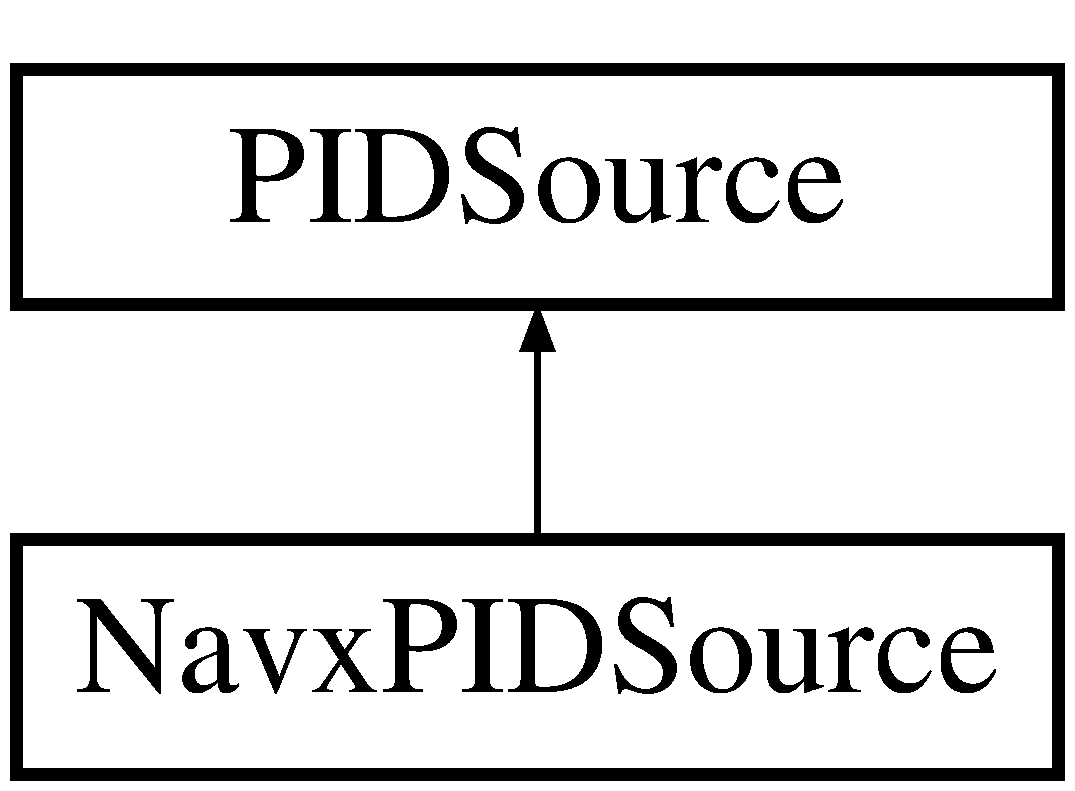
\includegraphics[height=2.000000cm]{class_navx_p_i_d_source}
\end{center}
\end{figure}
\subsection*{Public Member Functions}
\begin{DoxyCompactItemize}
\item 
\mbox{\Hypertarget{class_navx_p_i_d_source_a6d8910e49ac582970632e8ad20e9bc4b}\label{class_navx_p_i_d_source_a6d8910e49ac582970632e8ad20e9bc4b}} 
{\bfseries Navx\+P\+I\+D\+Source} (\hyperlink{class_robot_model}{Robot\+Model} $\ast$robot)
\item 
\mbox{\Hypertarget{class_navx_p_i_d_source_af3d4863c8b9338340739bf0d85371827}\label{class_navx_p_i_d_source_af3d4863c8b9338340739bf0d85371827}} 
double {\bfseries P\+I\+D\+Get} ()
\item 
\mbox{\Hypertarget{class_navx_p_i_d_source_ac9a334ad2d3d561f4b7e0d4686a1e3c3}\label{class_navx_p_i_d_source_ac9a334ad2d3d561f4b7e0d4686a1e3c3}} 
double {\bfseries Calculate\+Accumulated\+Yaw} ()
\item 
\mbox{\Hypertarget{class_navx_p_i_d_source_a553daca7b260429b4808791ff11ada54}\label{class_navx_p_i_d_source_a553daca7b260429b4808791ff11ada54}} 
void {\bfseries Reset\+Accumulated\+Yaw} ()
\end{DoxyCompactItemize}
\subsection*{Private Attributes}
\begin{DoxyCompactItemize}
\item 
\mbox{\Hypertarget{class_navx_p_i_d_source_a4e7fd0ab07e2a452de4e6dee8046a1e4}\label{class_navx_p_i_d_source_a4e7fd0ab07e2a452de4e6dee8046a1e4}} 
double {\bfseries curr\+Yaw\+\_\+}
\item 
\mbox{\Hypertarget{class_navx_p_i_d_source_ad23e187c9090d314887e3190d9f9f7a7}\label{class_navx_p_i_d_source_ad23e187c9090d314887e3190d9f9f7a7}} 
double {\bfseries last\+Yaw\+\_\+}
\item 
\mbox{\Hypertarget{class_navx_p_i_d_source_a44ed45bd794ad3011e951a47f1a2dbee}\label{class_navx_p_i_d_source_a44ed45bd794ad3011e951a47f1a2dbee}} 
double {\bfseries delta\+Yaw\+\_\+}
\item 
\mbox{\Hypertarget{class_navx_p_i_d_source_a034f1d606b899986012a67863cab39a3}\label{class_navx_p_i_d_source_a034f1d606b899986012a67863cab39a3}} 
double {\bfseries accumulated\+Yaw\+\_\+}
\item 
\mbox{\Hypertarget{class_navx_p_i_d_source_aaf8ac0b9fdad1ee64788ea7b50acc388}\label{class_navx_p_i_d_source_aaf8ac0b9fdad1ee64788ea7b50acc388}} 
\hyperlink{class_robot_model}{Robot\+Model} $\ast$ {\bfseries robot\+\_\+}
\end{DoxyCompactItemize}


The documentation for this class was generated from the following files\+:\begin{DoxyCompactItemize}
\item 
/\+Users/maggiewang/\+Space\+\_\+\+Cookies/spacecookies/frc2017/src/\+Auto/P\+I\+D\+Input\+Source.\+h\item 
/\+Users/maggiewang/\+Space\+\_\+\+Cookies/spacecookies/frc2017/src/\+Auto/P\+I\+D\+Input\+Source.\+cpp\end{DoxyCompactItemize}

\hypertarget{class_one_gear_high_shoot_mode}{}\section{One\+Gear\+High\+Shoot\+Mode Class Reference}
\label{class_one_gear_high_shoot_mode}\index{One\+Gear\+High\+Shoot\+Mode@{One\+Gear\+High\+Shoot\+Mode}}


The documentation for this class was generated from the following files\+:\begin{DoxyCompactItemize}
\item 
/\+Users/maggiewang/\+Space\+\_\+\+Cookies/spacecookies/frc2017/src/\+Auto/\+Modes/One\+Gear\+High\+Shoot\+Mode.\+h\item 
/\+Users/maggiewang/\+Space\+\_\+\+Cookies/spacecookies/frc2017/src/\+Auto/\+Modes/One\+Gear\+High\+Shoot\+Mode.\+cpp\end{DoxyCompactItemize}

\hypertarget{class_one_gear_mode}{}\section{One\+Gear\+Mode Class Reference}
\label{class_one_gear_mode}\index{One\+Gear\+Mode@{One\+Gear\+Mode}}
Inheritance diagram for One\+Gear\+Mode\+:\begin{figure}[H]
\begin{center}
\leavevmode
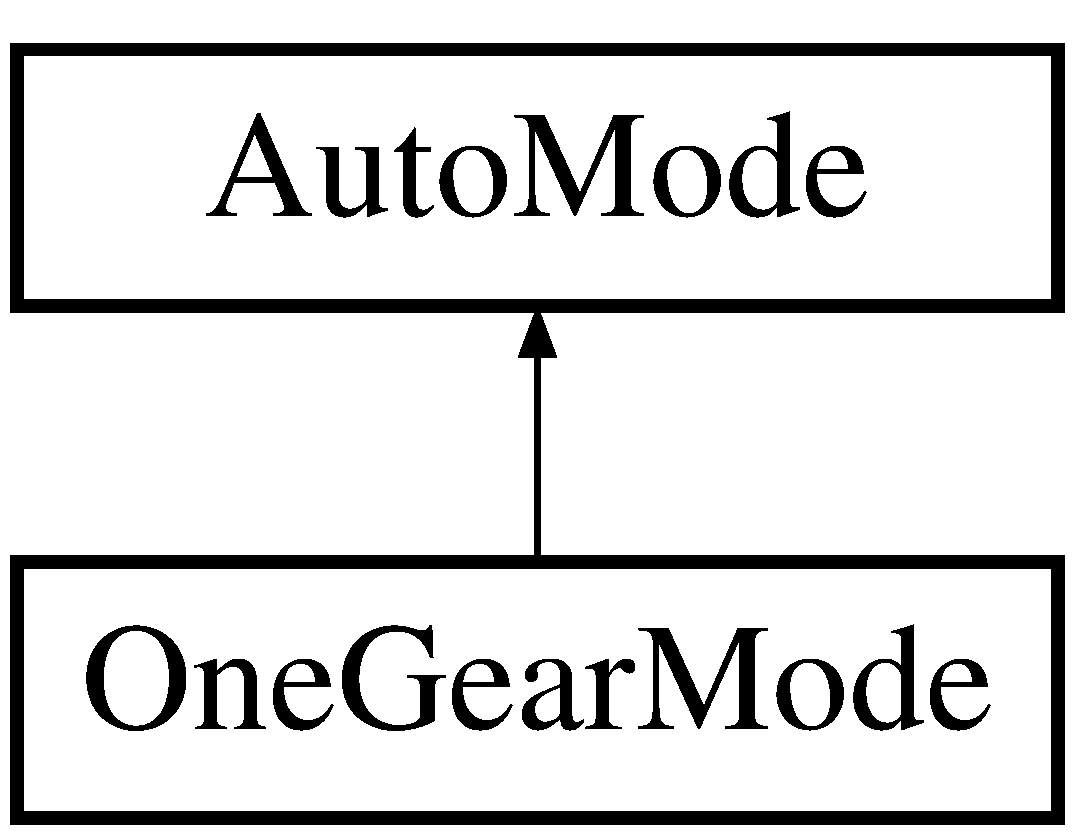
\includegraphics[height=2.000000cm]{class_one_gear_mode}
\end{center}
\end{figure}
\subsection*{Public Member Functions}
\begin{DoxyCompactItemize}
\item 
\hyperlink{class_one_gear_mode_a738b0127f542fb89c5a5976e534b6ef9}{One\+Gear\+Mode} (\hyperlink{class_robot_model}{Robot\+Model} $\ast$robot, \hyperlink{class_navx_p_i_d_source}{Navx\+P\+I\+D\+Source} $\ast$navx\+Source, \hyperlink{class_talon_encoder_p_i_d_source}{Talon\+Encoder\+P\+I\+D\+Source} $\ast$talon\+Source)
\item 
\mbox{\Hypertarget{class_one_gear_mode_a496910af844fa979cd7d879831dbb609}\label{class_one_gear_mode_a496910af844fa979cd7d879831dbb609}} 
void {\bfseries Create\+Queue} ()
\item 
void \hyperlink{class_one_gear_mode_a6e4583155a7f2c96f19e937d1315bdf8}{Init} ()
\item 
\mbox{\Hypertarget{class_one_gear_mode_a1aff75538d9985927fd0f10536b66aec}\label{class_one_gear_mode_a1aff75538d9985927fd0f10536b66aec}} 
void {\bfseries Refresh\+Ini} ()
\item 
\mbox{\Hypertarget{class_one_gear_mode_abbb66b39f2525f4de3d8cc0096d685a0}\label{class_one_gear_mode_abbb66b39f2525f4de3d8cc0096d685a0}} 
bool {\bfseries Is\+Done} ()
\end{DoxyCompactItemize}
\subsection*{Private Attributes}
\begin{DoxyCompactItemize}
\item 
\mbox{\Hypertarget{class_one_gear_mode_ad1b467771c98dc4e3156aea381390a00}\label{class_one_gear_mode_ad1b467771c98dc4e3156aea381390a00}} 
\hyperlink{class_robot_model}{Robot\+Model} $\ast$ {\bfseries robot\+\_\+}
\item 
\mbox{\Hypertarget{class_one_gear_mode_ad7d249a36949edf64d23759c626e4c98}\label{class_one_gear_mode_ad7d249a36949edf64d23759c626e4c98}} 
\hyperlink{class_auto_command}{Auto\+Command} $\ast$ {\bfseries first\+Command\+\_\+}
\item 
\mbox{\Hypertarget{class_one_gear_mode_ac943774ff57a1a71e70edb174ed57d17}\label{class_one_gear_mode_ac943774ff57a1a71e70edb174ed57d17}} 
\hyperlink{class_path_command}{Path\+Command} $\ast$ {\bfseries lift\+Path\+\_\+}
\item 
\mbox{\Hypertarget{class_one_gear_mode_a622236cb11ee049a22db35761fe2b07f}\label{class_one_gear_mode_a622236cb11ee049a22db35761fe2b07f}} 
\hyperlink{class_align_with_peg_command}{Align\+With\+Peg\+Command} $\ast$ {\bfseries align\+With\+Peg\+Command\+\_\+}
\item 
\mbox{\Hypertarget{class_one_gear_mode_a8d770f6dbe9a4895cc2c089325c979f0}\label{class_one_gear_mode_a8d770f6dbe9a4895cc2c089325c979f0}} 
\hyperlink{class_navx_p_i_d_source}{Navx\+P\+I\+D\+Source} $\ast$ {\bfseries navx\+Source\+\_\+}
\item 
\mbox{\Hypertarget{class_one_gear_mode_a1971e43e414dc22820e5db461f8f6a00}\label{class_one_gear_mode_a1971e43e414dc22820e5db461f8f6a00}} 
\hyperlink{class_talon_encoder_p_i_d_source}{Talon\+Encoder\+P\+I\+D\+Source} $\ast$ {\bfseries talon\+Source\+\_\+}
\end{DoxyCompactItemize}
\subsection*{Additional Inherited Members}


\subsection{Constructor \& Destructor Documentation}
\mbox{\Hypertarget{class_one_gear_mode_a738b0127f542fb89c5a5976e534b6ef9}\label{class_one_gear_mode_a738b0127f542fb89c5a5976e534b6ef9}} 
\index{One\+Gear\+Mode@{One\+Gear\+Mode}!One\+Gear\+Mode@{One\+Gear\+Mode}}
\index{One\+Gear\+Mode@{One\+Gear\+Mode}!One\+Gear\+Mode@{One\+Gear\+Mode}}
\subsubsection{\texorpdfstring{One\+Gear\+Mode()}{OneGearMode()}}
{\footnotesize\ttfamily One\+Gear\+Mode\+::\+One\+Gear\+Mode (\begin{DoxyParamCaption}\item[{\hyperlink{class_robot_model}{Robot\+Model} $\ast$}]{robot,  }\item[{\hyperlink{class_navx_p_i_d_source}{Navx\+P\+I\+D\+Source} $\ast$}]{navx\+Source,  }\item[{\hyperlink{class_talon_encoder_p_i_d_source}{Talon\+Encoder\+P\+I\+D\+Source} $\ast$}]{talon\+Source }\end{DoxyParamCaption})}

Constructs new \hyperlink{class_align_with_peg_command}{Align\+With\+Peg\+Command} 
\begin{DoxyParams}{Parameters}
{\em robot} & a \hyperlink{class_robot_model}{Robot\+Model} \\
\hline
\end{DoxyParams}


\subsection{Member Function Documentation}
\mbox{\Hypertarget{class_one_gear_mode_a6e4583155a7f2c96f19e937d1315bdf8}\label{class_one_gear_mode_a6e4583155a7f2c96f19e937d1315bdf8}} 
\index{One\+Gear\+Mode@{One\+Gear\+Mode}!Init@{Init}}
\index{Init@{Init}!One\+Gear\+Mode@{One\+Gear\+Mode}}
\subsubsection{\texorpdfstring{Init()}{Init()}}
{\footnotesize\ttfamily void One\+Gear\+Mode\+::\+Init (\begin{DoxyParamCaption}{ }\end{DoxyParamCaption})\hspace{0.3cm}{\ttfamily [virtual]}}

Initializes \hyperlink{class_align_with_peg_command}{Align\+With\+Peg\+Command} and sets current\+Command to first\+Command 

Implements \hyperlink{class_auto_mode}{Auto\+Mode}.



The documentation for this class was generated from the following files\+:\begin{DoxyCompactItemize}
\item 
/\+Users/maggiewang/\+Space\+\_\+\+Cookies/spacecookies/frc2017/src/\+Auto/\+Modes/One\+Gear\+Mode.\+h\item 
/\+Users/maggiewang/\+Space\+\_\+\+Cookies/spacecookies/frc2017/src/\+Auto/\+Modes/One\+Gear\+Mode.\+cpp\end{DoxyCompactItemize}

\hypertarget{class_path_command}{}\section{Path\+Command Class Reference}
\label{class_path_command}\index{Path\+Command@{Path\+Command}}
Inheritance diagram for Path\+Command\+:\begin{figure}[H]
\begin{center}
\leavevmode
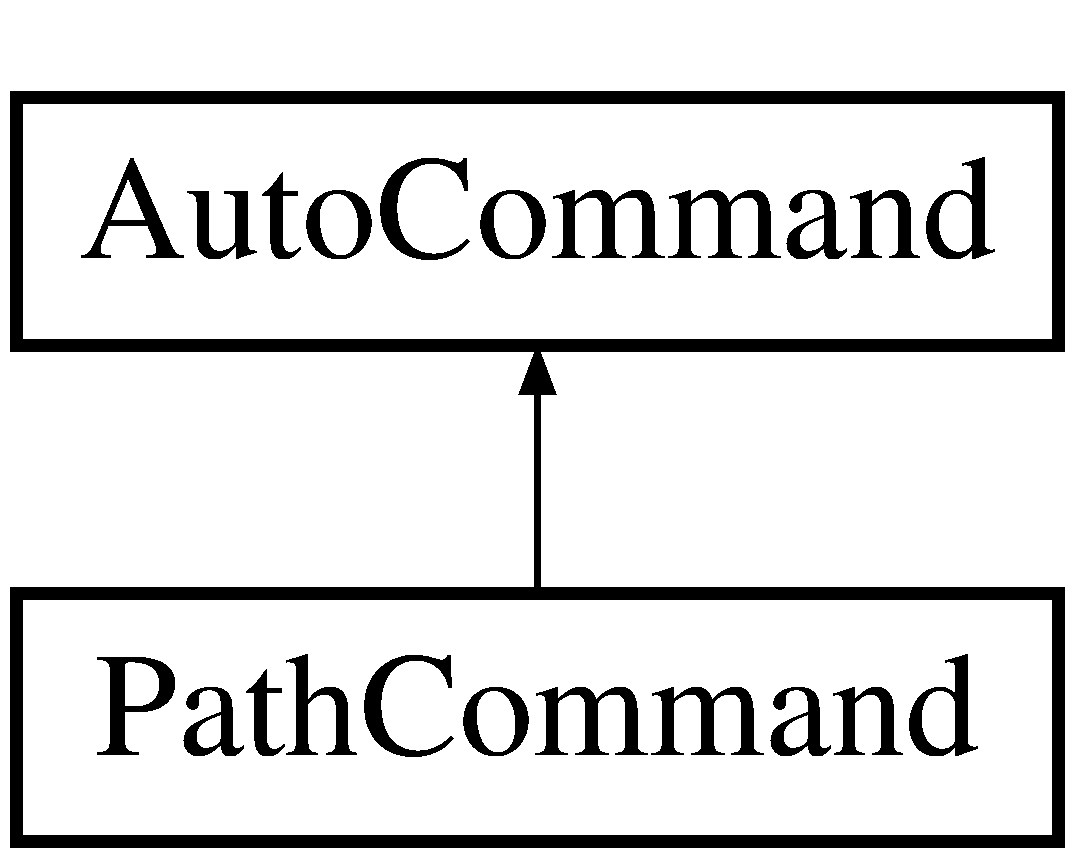
\includegraphics[height=2.000000cm]{class_path_command}
\end{center}
\end{figure}
\subsection*{Public Types}
\begin{DoxyCompactItemize}
\item 
\mbox{\Hypertarget{class_path_command_a16c9817753b2a9c1f171a6da90448424}\label{class_path_command_a16c9817753b2a9c1f171a6da90448424}} 
enum {\bfseries Path} \{ {\bfseries k\+Lift\+One}, 
{\bfseries k\+Lift\+Two}, 
{\bfseries k\+Lift\+Three}
 \}
\end{DoxyCompactItemize}
\subsection*{Public Member Functions}
\begin{DoxyCompactItemize}
\item 
\hyperlink{class_path_command_af13590c26630833220671975f3d2ffa9}{Path\+Command} (\hyperlink{class_robot_model}{Robot\+Model} $\ast$robot, Path path)
\item 
\mbox{\Hypertarget{class_path_command_af6b08e736ddda29d989fe484e9fd7383}\label{class_path_command_af6b08e736ddda29d989fe484e9fd7383}} 
void {\bfseries Init} ()
\item 
\mbox{\Hypertarget{class_path_command_a64f5ebbbe897a3305bdd9905e7b088f4}\label{class_path_command_a64f5ebbbe897a3305bdd9905e7b088f4}} 
void {\bfseries Update} (double curr\+Time\+Sec, double delta\+Time\+Sec)
\item 
\mbox{\Hypertarget{class_path_command_a29e919cef5f6ba460060c6252d2c2910}\label{class_path_command_a29e919cef5f6ba460060c6252d2c2910}} 
bool {\bfseries Is\+Done} ()
\end{DoxyCompactItemize}
\subsection*{Private Attributes}
\begin{DoxyCompactItemize}
\item 
\mbox{\Hypertarget{class_path_command_aa6a8d5bdb0c926243b0f5ccc86ad92ff}\label{class_path_command_aa6a8d5bdb0c926243b0f5ccc86ad92ff}} 
\hyperlink{class_robot_model}{Robot\+Model} $\ast$ {\bfseries robot\+\_\+}
\item 
\mbox{\Hypertarget{class_path_command_a8fbec2fd0e2c338fab60a437c018a7a0}\label{class_path_command_a8fbec2fd0e2c338fab60a437c018a7a0}} 
Path {\bfseries path\+\_\+}
\item 
\mbox{\Hypertarget{class_path_command_a5e0ad49c59397dd781fe49fd010a534e}\label{class_path_command_a5e0ad49c59397dd781fe49fd010a534e}} 
int {\bfseries length\+Of\+Left\+Motion\+Profile\+\_\+}
\item 
\mbox{\Hypertarget{class_path_command_a7e302dc5bdc6863670c6c808227af2ce}\label{class_path_command_a7e302dc5bdc6863670c6c808227af2ce}} 
int {\bfseries length\+Of\+Right\+Motion\+Profile\+\_\+}
\item 
\mbox{\Hypertarget{class_path_command_abc8680e2a7fef01f3f524d492a2414e6}\label{class_path_command_abc8680e2a7fef01f3f524d492a2414e6}} 
double {\bfseries left\+Motion\+Profile\+\_\+} \mbox{[}$\,$\mbox{]}\mbox{[}3\mbox{]}
\item 
\mbox{\Hypertarget{class_path_command_a7baa75d4c65c1a41bbb1db5cf81cae39}\label{class_path_command_a7baa75d4c65c1a41bbb1db5cf81cae39}} 
double {\bfseries right\+Motion\+Profile\+\_\+} \mbox{[}$\,$\mbox{]}\mbox{[}3\mbox{]}
\item 
\mbox{\Hypertarget{class_path_command_a7849e4b9ed084e5906894f0d9d6e2c34}\label{class_path_command_a7849e4b9ed084e5906894f0d9d6e2c34}} 
\hyperlink{class_motion_profile_executor}{Motion\+Profile\+Executor} $\ast$ {\bfseries left\+Motion\+Profile\+Executor\+\_\+}
\item 
\mbox{\Hypertarget{class_path_command_a244b142d11c2a135ae1d0e50ed0b2979}\label{class_path_command_a244b142d11c2a135ae1d0e50ed0b2979}} 
\hyperlink{class_motion_profile_executor}{Motion\+Profile\+Executor} $\ast$ {\bfseries right\+Motion\+Profile\+Executor\+\_\+}
\item 
\mbox{\Hypertarget{class_path_command_a92a777a063e9beecfb3461f54306c78f}\label{class_path_command_a92a777a063e9beecfb3461f54306c78f}} 
bool {\bfseries is\+Done\+\_\+}
\end{DoxyCompactItemize}


\subsection{Constructor \& Destructor Documentation}
\mbox{\Hypertarget{class_path_command_af13590c26630833220671975f3d2ffa9}\label{class_path_command_af13590c26630833220671975f3d2ffa9}} 
\index{Path\+Command@{Path\+Command}!Path\+Command@{Path\+Command}}
\index{Path\+Command@{Path\+Command}!Path\+Command@{Path\+Command}}
\subsubsection{\texorpdfstring{Path\+Command()}{PathCommand()}}
{\footnotesize\ttfamily Path\+Command\+::\+Path\+Command (\begin{DoxyParamCaption}\item[{\hyperlink{class_robot_model}{Robot\+Model} $\ast$}]{robot,  }\item[{Path}]{path }\end{DoxyParamCaption})}

Constructor that generates a \hyperlink{class_path_command}{Path\+Command} 
\begin{DoxyParams}{Parameters}
{\em robot} & a \hyperlink{class_robot_model}{Robot\+Model} \\
\hline
{\em Path} & a path of waypoints generated by motion profile \\
\hline
\end{DoxyParams}


The documentation for this class was generated from the following files\+:\begin{DoxyCompactItemize}
\item 
/\+Users/maggiewang/\+Space\+\_\+\+Cookies/spacecookies/frc2017/src/\+Auto/\+Commands/Path\+Command.\+h\item 
/\+Users/maggiewang/\+Space\+\_\+\+Cookies/spacecookies/frc2017/src/\+Auto/\+Commands/Path\+Command.\+cpp\end{DoxyCompactItemize}

\hypertarget{class_pivot_command}{}\section{Pivot\+Command Class Reference}
\label{class_pivot_command}\index{Pivot\+Command@{Pivot\+Command}}


{\ttfamily \#include $<$Pivot\+Command.\+h$>$}

Inheritance diagram for Pivot\+Command\+:\begin{figure}[H]
\begin{center}
\leavevmode
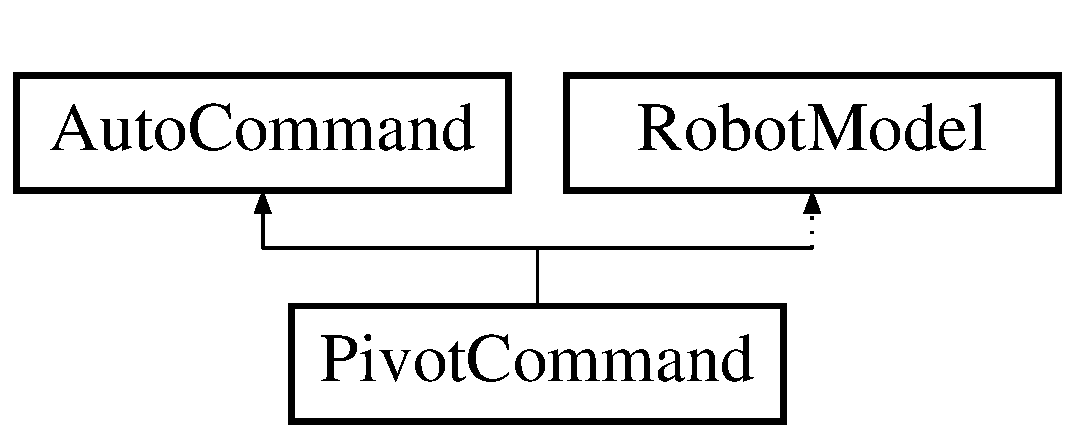
\includegraphics[height=2.000000cm]{class_pivot_command}
\end{center}
\end{figure}
\subsection*{Public Member Functions}
\begin{DoxyCompactItemize}
\item 
\hyperlink{class_pivot_command_aeed6d5f91fade3124c4a66080edad50d}{Pivot\+Command} (\hyperlink{class_robot_model}{Robot\+Model} $\ast$robot, double desired\+Angle, bool is\+Absolute\+Position, \hyperlink{class_navx_p_i_d_source}{Navx\+P\+I\+D\+Source} $\ast$navx\+Source)
\item 
\mbox{\Hypertarget{class_pivot_command_a4bc3497678e5fdc84e0ec545f87fcd2a}\label{class_pivot_command_a4bc3497678e5fdc84e0ec545f87fcd2a}} 
void {\bfseries Init} ()
\item 
\mbox{\Hypertarget{class_pivot_command_a728a96471b607920a8e3581b15c2a6ed}\label{class_pivot_command_a728a96471b607920a8e3581b15c2a6ed}} 
void {\bfseries Reset} ()
\item 
\mbox{\Hypertarget{class_pivot_command_aabcc35cb7b9a7401285f800475d79bb1}\label{class_pivot_command_aabcc35cb7b9a7401285f800475d79bb1}} 
void {\bfseries Refresh\+Ini} ()
\item 
\mbox{\Hypertarget{class_pivot_command_ab43066cd70a708f342f53f94558acf98}\label{class_pivot_command_ab43066cd70a708f342f53f94558acf98}} 
void {\bfseries Update} (double curr\+Time\+Sec, double delta\+Time\+Sec)
\item 
\mbox{\Hypertarget{class_pivot_command_acc8ed3e6a76a19a05201131f0bd7ccc5}\label{class_pivot_command_acc8ed3e6a76a19a05201131f0bd7ccc5}} 
bool {\bfseries Is\+Done} ()
\end{DoxyCompactItemize}
\subsection*{Private Member Functions}
\begin{DoxyCompactItemize}
\item 
double \hyperlink{class_pivot_command_a56f0c011b2a744f1ed0a2b5cb301cdb2}{Calculate\+Delta\+Angle} (double desired\+Angle)
\end{DoxyCompactItemize}
\subsection*{Private Attributes}
\begin{DoxyCompactItemize}
\item 
\mbox{\Hypertarget{class_pivot_command_af19ee15f8b4d195bf02fbc697eba1641}\label{class_pivot_command_af19ee15f8b4d195bf02fbc697eba1641}} 
double {\bfseries p\+Fac\+\_\+}
\item 
\mbox{\Hypertarget{class_pivot_command_a8a4c07edea472ab21522cca70fe531a2}\label{class_pivot_command_a8a4c07edea472ab21522cca70fe531a2}} 
double {\bfseries i\+Fac\+\_\+}
\item 
\mbox{\Hypertarget{class_pivot_command_a076fe76ca613db3f914408607e91d7bc}\label{class_pivot_command_a076fe76ca613db3f914408607e91d7bc}} 
double {\bfseries d\+Fac\+\_\+}
\item 
\mbox{\Hypertarget{class_pivot_command_aaf3bb529c25ee4d2ed040fdacb794d1f}\label{class_pivot_command_aaf3bb529c25ee4d2ed040fdacb794d1f}} 
double {\bfseries desired\+Delta\+Angle\+\_\+}
\item 
\mbox{\Hypertarget{class_pivot_command_aa0fc36f13532c492f5e86b4d5d0be93e}\label{class_pivot_command_aa0fc36f13532c492f5e86b4d5d0be93e}} 
double {\bfseries init\+Yaw\+\_\+}
\item 
\mbox{\Hypertarget{class_pivot_command_a40b669643047869696913de119de0347}\label{class_pivot_command_a40b669643047869696913de119de0347}} 
bool {\bfseries is\+Done\+\_\+}
\item 
\mbox{\Hypertarget{class_pivot_command_ad1fd030762a6b95d8c8ccad7375c2dcb}\label{class_pivot_command_ad1fd030762a6b95d8c8ccad7375c2dcb}} 
\hyperlink{class_robot_model}{Robot\+Model} $\ast$ {\bfseries robot\+\_\+}
\item 
\mbox{\Hypertarget{class_pivot_command_ae2fcdfa0e3be71c8b06a42440dbe3003}\label{class_pivot_command_ae2fcdfa0e3be71c8b06a42440dbe3003}} 
P\+I\+D\+Controller $\ast$ {\bfseries pivot\+P\+I\+D\+\_\+}
\item 
\mbox{\Hypertarget{class_pivot_command_a5fd31234c07b80cc3ffddb3ce28bc49b}\label{class_pivot_command_a5fd31234c07b80cc3ffddb3ce28bc49b}} 
\hyperlink{class_navx_p_i_d_source}{Navx\+P\+I\+D\+Source} $\ast$ {\bfseries navx\+Source\+\_\+}
\item 
\mbox{\Hypertarget{class_pivot_command_a590ea9a551076484febed96b6f7d9a64}\label{class_pivot_command_a590ea9a551076484febed96b6f7d9a64}} 
\hyperlink{class_pivot_p_i_d_talon_output}{Pivot\+P\+I\+D\+Talon\+Output} $\ast$ {\bfseries talon\+Output\+\_\+}
\item 
\mbox{\Hypertarget{class_pivot_command_a5ec7f0d7b577e7830251e78a895798b5}\label{class_pivot_command_a5ec7f0d7b577e7830251e78a895798b5}} 
double {\bfseries pivot\+Command\+Start\+Time\+\_\+}
\item 
\mbox{\Hypertarget{class_pivot_command_aa0b7e3b621788df09e8f2cc3c184b858}\label{class_pivot_command_aa0b7e3b621788df09e8f2cc3c184b858}} 
double {\bfseries min\+Drive\+Pivot\+Output\+\_\+}
\end{DoxyCompactItemize}
\subsection*{Additional Inherited Members}


\subsection{Detailed Description}
A class implementing Pivot P\+ID the W\+P\+I\+Library P\+ID Controller 

\subsection{Constructor \& Destructor Documentation}
\mbox{\Hypertarget{class_pivot_command_aeed6d5f91fade3124c4a66080edad50d}\label{class_pivot_command_aeed6d5f91fade3124c4a66080edad50d}} 
\index{Pivot\+Command@{Pivot\+Command}!Pivot\+Command@{Pivot\+Command}}
\index{Pivot\+Command@{Pivot\+Command}!Pivot\+Command@{Pivot\+Command}}
\subsubsection{\texorpdfstring{Pivot\+Command()}{PivotCommand()}}
{\footnotesize\ttfamily Pivot\+Command\+::\+Pivot\+Command (\begin{DoxyParamCaption}\item[{\hyperlink{class_robot_model}{Robot\+Model} $\ast$}]{robot,  }\item[{double}]{desired\+Angle,  }\item[{bool}]{is\+Absolute\+Position,  }\item[{\hyperlink{class_navx_p_i_d_source}{Navx\+P\+I\+D\+Source} $\ast$}]{navx\+Source }\end{DoxyParamCaption})}

\hyperlink{class_pivot_command}{Pivot\+Command} constructor that gives the desired turn and whether or not it is absolute position 
\begin{DoxyParams}{Parameters}
{\em robot} & a \hyperlink{class_robot_model}{Robot\+Model} \\
\hline
{\em desired\+Angle} & a double that is the angle of the turn \\
\hline
{\em is\+Absolute\+Position} & a bool that represents whether the angle is absolute position or delta angle \\
\hline
{\em navx\+Source} & a \hyperlink{class_navx_p_i_d_source}{Navx\+P\+I\+D\+Source} \\
\hline
\end{DoxyParams}


\subsection{Member Function Documentation}
\mbox{\Hypertarget{class_pivot_command_a56f0c011b2a744f1ed0a2b5cb301cdb2}\label{class_pivot_command_a56f0c011b2a744f1ed0a2b5cb301cdb2}} 
\index{Pivot\+Command@{Pivot\+Command}!Calculate\+Delta\+Angle@{Calculate\+Delta\+Angle}}
\index{Calculate\+Delta\+Angle@{Calculate\+Delta\+Angle}!Pivot\+Command@{Pivot\+Command}}
\subsubsection{\texorpdfstring{Calculate\+Delta\+Angle()}{CalculateDeltaAngle()}}
{\footnotesize\ttfamily double Pivot\+Command\+::\+Calculate\+Delta\+Angle (\begin{DoxyParamCaption}\item[{double}]{desired\+Angle }\end{DoxyParamCaption})\hspace{0.3cm}{\ttfamily [private]}}

Calculating the value of delta angle if the angle is absolute position. 
\begin{DoxyParams}{Parameters}
{\em desired\+Angle} & a double is the original angle passed in from constructor. \\
\hline
\end{DoxyParams}
\begin{DoxyReturn}{Returns}
delta\+Angle which is the amount we have to turn to get to the absolute position 
\end{DoxyReturn}


The documentation for this class was generated from the following files\+:\begin{DoxyCompactItemize}
\item 
/\+Users/maggiewang/\+Space\+\_\+\+Cookies/spacecookies/frc2017/src/\+Auto/\+Commands/Pivot\+Command.\+h\item 
/\+Users/maggiewang/\+Space\+\_\+\+Cookies/spacecookies/frc2017/src/\+Auto/\+Commands/Pivot\+Command.\+cpp\end{DoxyCompactItemize}

\hypertarget{class_pivot_p_i_d_talon_output}{}\section{Pivot\+P\+I\+D\+Talon\+Output Class Reference}
\label{class_pivot_p_i_d_talon_output}\index{Pivot\+P\+I\+D\+Talon\+Output@{Pivot\+P\+I\+D\+Talon\+Output}}
Inheritance diagram for Pivot\+P\+I\+D\+Talon\+Output\+:\begin{figure}[H]
\begin{center}
\leavevmode
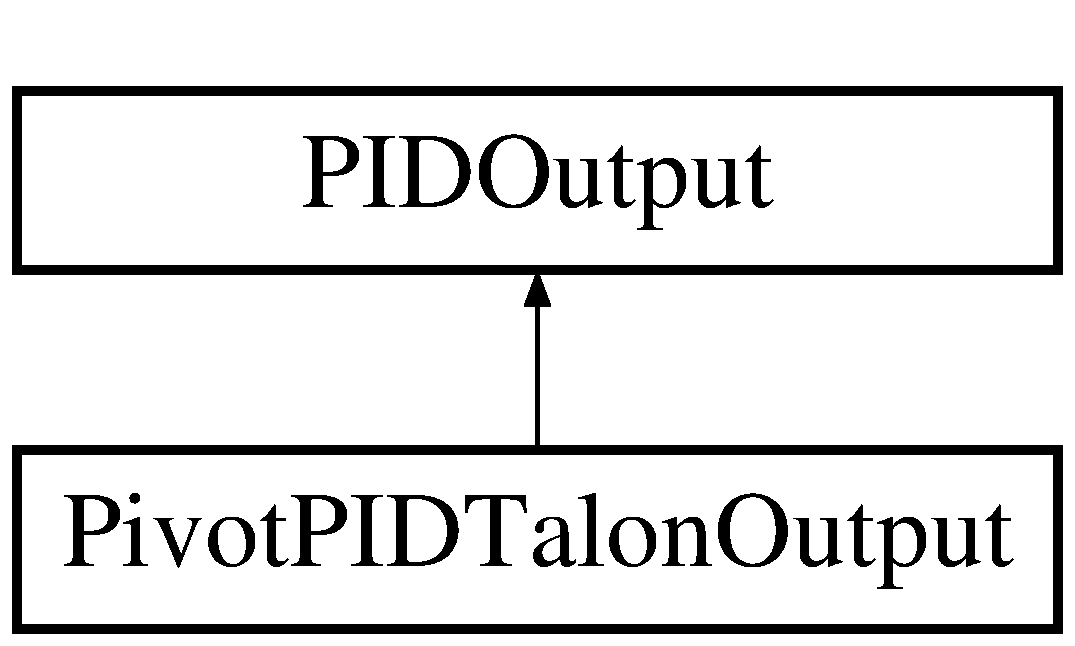
\includegraphics[height=2.000000cm]{class_pivot_p_i_d_talon_output}
\end{center}
\end{figure}
\subsection*{Public Member Functions}
\begin{DoxyCompactItemize}
\item 
\mbox{\Hypertarget{class_pivot_p_i_d_talon_output_ac7dff318a32bf616f397f6edf642b17e}\label{class_pivot_p_i_d_talon_output_ac7dff318a32bf616f397f6edf642b17e}} 
{\bfseries Pivot\+P\+I\+D\+Talon\+Output} (\hyperlink{class_robot_model}{Robot\+Model} $\ast$robot)
\item 
\mbox{\Hypertarget{class_pivot_p_i_d_talon_output_a8a2c7a13ef615ad01d00fecc6a16f715}\label{class_pivot_p_i_d_talon_output_a8a2c7a13ef615ad01d00fecc6a16f715}} 
void {\bfseries P\+I\+D\+Write} (double output)
\item 
\mbox{\Hypertarget{class_pivot_p_i_d_talon_output_a19563bcd7d8afaae782ef167e4a3a973}\label{class_pivot_p_i_d_talon_output_a19563bcd7d8afaae782ef167e4a3a973}} 
double {\bfseries Get\+Output} ()
\end{DoxyCompactItemize}
\subsection*{Private Attributes}
\begin{DoxyCompactItemize}
\item 
\mbox{\Hypertarget{class_pivot_p_i_d_talon_output_a21f494514211fabf65c2615dce434db4}\label{class_pivot_p_i_d_talon_output_a21f494514211fabf65c2615dce434db4}} 
\hyperlink{class_robot_model}{Robot\+Model} $\ast$ {\bfseries robot\+\_\+}
\item 
\mbox{\Hypertarget{class_pivot_p_i_d_talon_output_a1962bd005ba3a4e0909695a4a321fdf0}\label{class_pivot_p_i_d_talon_output_a1962bd005ba3a4e0909695a4a321fdf0}} 
double {\bfseries output\+\_\+}
\end{DoxyCompactItemize}


The documentation for this class was generated from the following files\+:\begin{DoxyCompactItemize}
\item 
/\+Users/maggiewang/\+Space\+\_\+\+Cookies/spacecookies/frc2017/src/\+Auto/\+Commands/Pivot\+Command.\+h\item 
/\+Users/maggiewang/\+Space\+\_\+\+Cookies/spacecookies/frc2017/src/\+Auto/\+Commands/Pivot\+Command.\+cpp\end{DoxyCompactItemize}

\hypertarget{class_remote_control}{}\section{Remote\+Control Class Reference}
\label{class_remote_control}\index{Remote\+Control@{Remote\+Control}}
Inheritance diagram for Remote\+Control\+:\begin{figure}[H]
\begin{center}
\leavevmode
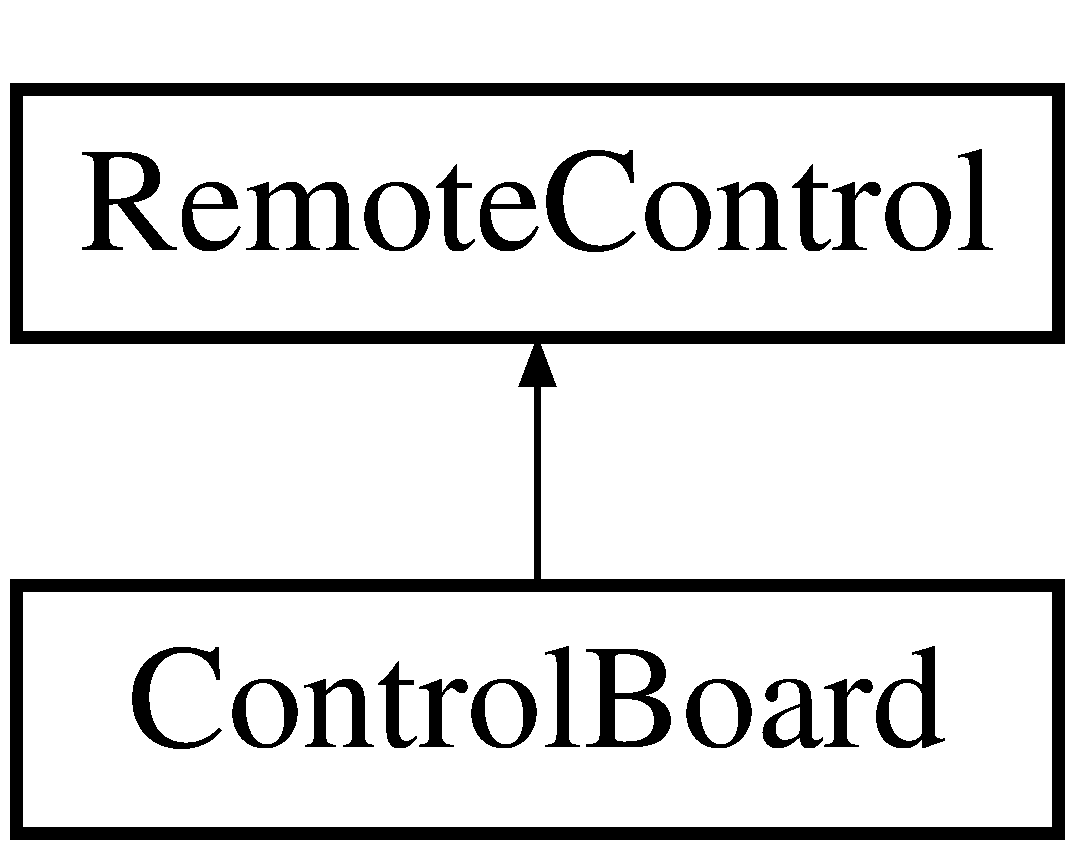
\includegraphics[height=2.000000cm]{class_remote_control}
\end{center}
\end{figure}
\subsection*{Public Types}
\begin{DoxyCompactItemize}
\item 
\mbox{\Hypertarget{class_remote_control_ad7f2809f8e524bd001ffd11b08ce178f}\label{class_remote_control_ad7f2809f8e524bd001ffd11b08ce178f}} 
enum {\bfseries Joysticks} \{ {\bfseries k\+Right\+Joy}, 
{\bfseries k\+Left\+Joy}
 \}
\item 
\mbox{\Hypertarget{class_remote_control_a3442e12f9e38389adcf2cc5bf9bd5650}\label{class_remote_control_a3442e12f9e38389adcf2cc5bf9bd5650}} 
enum {\bfseries Axes} \{ {\bfseries kX}, 
{\bfseries kY}
 \}
\end{DoxyCompactItemize}
\subsection*{Public Member Functions}
\begin{DoxyCompactItemize}
\item 
\mbox{\Hypertarget{class_remote_control_a7dbf96cb324ba35eed5d321b20a684cc}\label{class_remote_control_a7dbf96cb324ba35eed5d321b20a684cc}} 
virtual void {\bfseries Read\+Controls} ()=0
\item 
\mbox{\Hypertarget{class_remote_control_a8ab237f494be1e03acf73c7f1a074dc4}\label{class_remote_control_a8ab237f494be1e03acf73c7f1a074dc4}} 
virtual double {\bfseries Get\+Joystick\+Value} (Joysticks j, Axes a)=0
\item 
\mbox{\Hypertarget{class_remote_control_ac4a415757aa25c0aaa51c079beb8b5ec}\label{class_remote_control_ac4a415757aa25c0aaa51c079beb8b5ec}} 
virtual bool {\bfseries Get\+Reverse\+Drive\+Desired} ()=0
\item 
\mbox{\Hypertarget{class_remote_control_a6bc6abea1db8060576faf0bfd764cd9c}\label{class_remote_control_a6bc6abea1db8060576faf0bfd764cd9c}} 
virtual bool {\bfseries Get\+Gear\+Shift\+Desired} ()=0
\item 
\mbox{\Hypertarget{class_remote_control_a2899dfb8cf4f9530d11de7962293f2bf}\label{class_remote_control_a2899dfb8cf4f9530d11de7962293f2bf}} 
virtual bool {\bfseries Get\+Arcade\+Drive\+Desired} ()=0
\item 
\mbox{\Hypertarget{class_remote_control_a20ad515a8b9c6f842844d3081ce29e1c}\label{class_remote_control_a20ad515a8b9c6f842844d3081ce29e1c}} 
virtual bool {\bfseries Get\+Quick\+Turn\+Desired} ()=0
\end{DoxyCompactItemize}


The documentation for this class was generated from the following file\+:\begin{DoxyCompactItemize}
\item 
/\+Users/maggiewang/\+Space\+\_\+\+Cookies/spacecookies/frc2017/src/\+Driver\+Station/Remote\+Control.\+h\end{DoxyCompactItemize}

\hypertarget{class_robot_model}{}\section{Robot\+Model Class Reference}
\label{class_robot_model}\index{Robot\+Model@{Robot\+Model}}
Inheritance diagram for Robot\+Model\+:\begin{figure}[H]
\begin{center}
\leavevmode
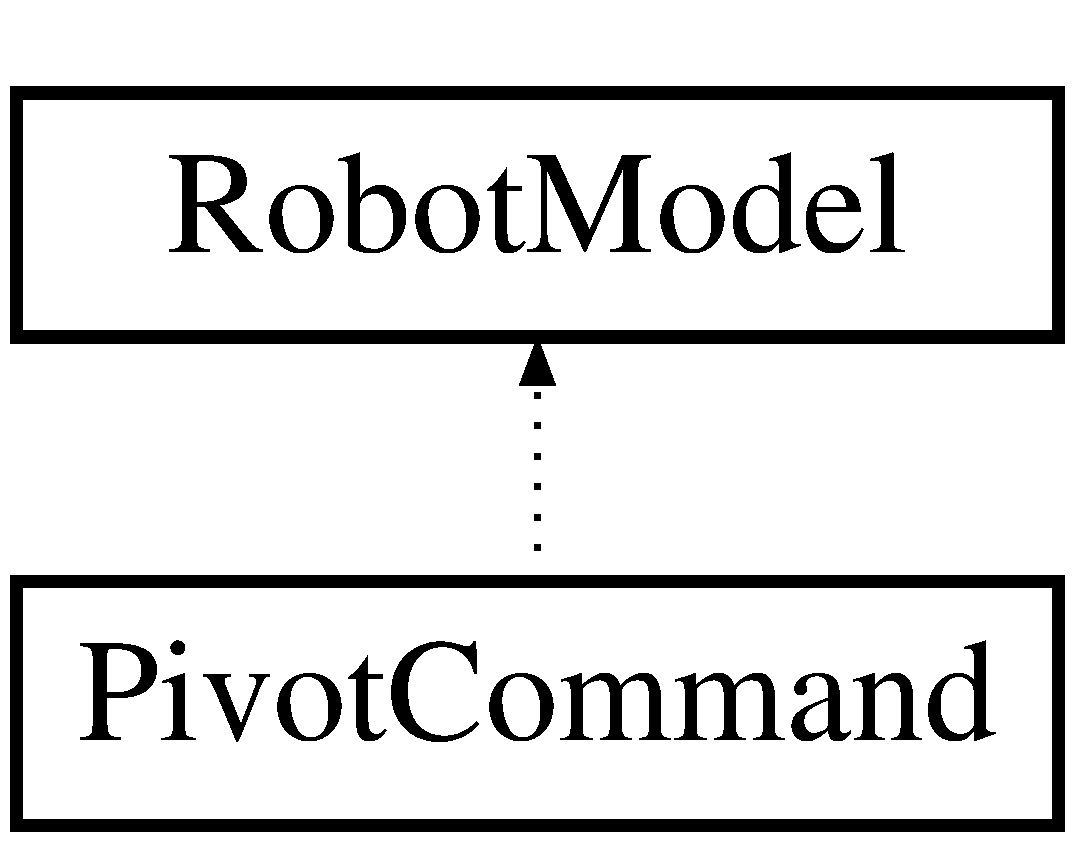
\includegraphics[height=2.000000cm]{class_robot_model}
\end{center}
\end{figure}
\subsection*{Public Types}
\begin{DoxyCompactItemize}
\item 
\mbox{\Hypertarget{class_robot_model_a35905ffde364a186d02ec199857ce170}\label{class_robot_model_a35905ffde364a186d02ec199857ce170}} 
enum {\bfseries Wheels} \{ {\bfseries k\+Left\+Wheels}, 
{\bfseries k\+Right\+Wheels}, 
{\bfseries k\+All\+Wheels}
 \}
\end{DoxyCompactItemize}
\subsection*{Public Member Functions}
\begin{DoxyCompactItemize}
\item 
\mbox{\Hypertarget{class_robot_model_a12fcf976a7f338c4d7dcba8b2765bbca}\label{class_robot_model_a12fcf976a7f338c4d7dcba8b2765bbca}} 
void {\bfseries Reset\+Timer} ()
\item 
\mbox{\Hypertarget{class_robot_model_a53211a6f086c2934f29696097e33c13c}\label{class_robot_model_a53211a6f086c2934f29696097e33c13c}} 
double {\bfseries Get\+Time} ()
\item 
\mbox{\Hypertarget{class_robot_model_a5c46e71b1ecd43497fa6a552edee2850}\label{class_robot_model_a5c46e71b1ecd43497fa6a552edee2850}} 
void {\bfseries Set\+Talon\+P\+I\+D\+Config} (Wheels wheel, double p\+Fac, double i\+Fac, double d\+Fac, double f\+Fac)
\item 
\mbox{\Hypertarget{class_robot_model_a9e82ace9c9249288fd82b58a6ec1288e}\label{class_robot_model_a9e82ace9c9249288fd82b58a6ec1288e}} 
void {\bfseries Set\+Motion\+Profile} ()
\item 
\mbox{\Hypertarget{class_robot_model_a00aec98c4ed4de1e7f48c2482fdad2a1}\label{class_robot_model_a00aec98c4ed4de1e7f48c2482fdad2a1}} 
void {\bfseries Set\+Percent\+V\+Drive} ()
\item 
\mbox{\Hypertarget{class_robot_model_a98f996b588768ca75ca0cf2dddcd217c}\label{class_robot_model_a98f996b588768ca75ca0cf2dddcd217c}} 
void {\bfseries Set\+Drive\+Values} (Wheels wheel, double value)
\item 
\mbox{\Hypertarget{class_robot_model_ac34a7071a6f8e1cccc5b16acd966d512}\label{class_robot_model_ac34a7071a6f8e1cccc5b16acd966d512}} 
void {\bfseries Clear\+Motion\+Profile\+Trajectories} ()
\item 
\mbox{\Hypertarget{class_robot_model_a79245b48351252c90a9ff994e9b40ebb}\label{class_robot_model_a79245b48351252c90a9ff994e9b40ebb}} 
double {\bfseries Get\+Drive\+Encoder\+Value} (Wheels wheel)
\item 
\mbox{\Hypertarget{class_robot_model_a4fb9600c4ba5dc1594cd703bcc069683}\label{class_robot_model_a4fb9600c4ba5dc1594cd703bcc069683}} 
double {\bfseries Get\+Left\+Distance} ()
\item 
\mbox{\Hypertarget{class_robot_model_acb69c744e99d5c938f983bf6da66f6f9}\label{class_robot_model_acb69c744e99d5c938f983bf6da66f6f9}} 
double {\bfseries Get\+Right\+Distance} ()
\item 
\mbox{\Hypertarget{class_robot_model_a48702daa83b141eb0dd1dc6f0fd75c35}\label{class_robot_model_a48702daa83b141eb0dd1dc6f0fd75c35}} 
double {\bfseries Get\+Navx\+Yaw} ()
\item 
\mbox{\Hypertarget{class_robot_model_a49cf4f33221954e0efbfc14dae477595}\label{class_robot_model_a49cf4f33221954e0efbfc14dae477595}} 
void {\bfseries Zero\+Navx\+Yaw} ()
\item 
\mbox{\Hypertarget{class_robot_model_a3f5ac4f1f526f4610573fc3dbcdc722c}\label{class_robot_model_a3f5ac4f1f526f4610573fc3dbcdc722c}} 
void {\bfseries Refresh\+Ini} ()
\item 
\mbox{\Hypertarget{class_robot_model_a66eb15697284c9f84e81274c42074f98}\label{class_robot_model_a66eb15697284c9f84e81274c42074f98}} 
double {\bfseries Get\+Feeder\+Output} ()
\item 
\mbox{\Hypertarget{class_robot_model_a60b4ba0082d91ec75d49584532ce17d5}\label{class_robot_model_a60b4ba0082d91ec75d49584532ce17d5}} 
void {\bfseries Set\+Feeder\+Output} (double output)
\item 
\mbox{\Hypertarget{class_robot_model_a83cf79ec3a2c2f89846bbc8f1371d061}\label{class_robot_model_a83cf79ec3a2c2f89846bbc8f1371d061}} 
double {\bfseries Get\+Climber\+Output} ()
\item 
\mbox{\Hypertarget{class_robot_model_a3c3562ec10706ee53e7d304c7f69e136}\label{class_robot_model_a3c3562ec10706ee53e7d304c7f69e136}} 
void {\bfseries Set\+Climber\+Output} (double output)
\item 
\mbox{\Hypertarget{class_robot_model_a08ca5e903c521ab19e40dc7ab34ccf16}\label{class_robot_model_a08ca5e903c521ab19e40dc7ab34ccf16}} 
Encoder $\ast$ {\bfseries Get\+Flywheel\+Encoder} ()
\item 
\mbox{\Hypertarget{class_robot_model_a421afc34c2fa51b2d4a0fb26d0115e0a}\label{class_robot_model_a421afc34c2fa51b2d4a0fb26d0115e0a}} 
Encoder $\ast$ {\bfseries Get\+Intake\+Encoder} ()
\item 
\mbox{\Hypertarget{class_robot_model_a2a91026e2bbd046d355c2619990ac537}\label{class_robot_model_a2a91026e2bbd046d355c2619990ac537}} 
Victor $\ast$ {\bfseries Get\+Flywheel\+Motor} ()
\item 
\mbox{\Hypertarget{class_robot_model_a2e186d42b8fcbee137e01072dbd160a1}\label{class_robot_model_a2e186d42b8fcbee137e01072dbd160a1}} 
Victor $\ast$ {\bfseries Get\+Intake\+Motor} ()
\item 
\mbox{\Hypertarget{class_robot_model_a87b1558491f004d77a0d5fd308cae225}\label{class_robot_model_a87b1558491f004d77a0d5fd308cae225}} 
bool {\bfseries Get\+Gear\+In\+Robot} ()
\item 
\mbox{\Hypertarget{class_robot_model_af4fb53182642778b932b510fe2b9bec1}\label{class_robot_model_af4fb53182642778b932b510fe2b9bec1}} 
void {\bfseries Set\+Gear\+In\+Robot} ()
\end{DoxyCompactItemize}
\subsection*{Public Attributes}
\begin{DoxyCompactItemize}
\item 
\mbox{\Hypertarget{class_robot_model_ab717f68553a5a87e822104526c2c384e}\label{class_robot_model_ab717f68553a5a87e822104526c2c384e}} 
Ini $\ast$ {\bfseries pini}
\item 
\mbox{\Hypertarget{class_robot_model_a4b24c35077efb8134a6c8c39dbec0a94}\label{class_robot_model_a4b24c35077efb8134a6c8c39dbec0a94}} 
C\+A\+N\+Talon $\ast$ {\bfseries left\+Master\+\_\+}
\item 
\mbox{\Hypertarget{class_robot_model_a2dba54867affd957c357da252767cb12}\label{class_robot_model_a2dba54867affd957c357da252767cb12}} 
C\+A\+N\+Talon $\ast$ {\bfseries right\+Master\+\_\+}
\item 
\mbox{\Hypertarget{class_robot_model_ab8412b3ded9c56ff0dc064c6bd717236}\label{class_robot_model_ab8412b3ded9c56ff0dc064c6bd717236}} 
C\+A\+N\+Talon $\ast$ {\bfseries left\+Slave\+\_\+}
\item 
\mbox{\Hypertarget{class_robot_model_abfeab5e7111c28a26b070e811c1a5fd2}\label{class_robot_model_abfeab5e7111c28a26b070e811c1a5fd2}} 
C\+A\+N\+Talon $\ast$ {\bfseries right\+Slave\+\_\+}
\end{DoxyCompactItemize}
\subsection*{Private Attributes}
\begin{DoxyCompactItemize}
\item 
\mbox{\Hypertarget{class_robot_model_a31809e8f8fddca2bf39ed07a2a6e9450}\label{class_robot_model_a31809e8f8fddca2bf39ed07a2a6e9450}} 
Timer $\ast$ {\bfseries timer\+\_\+}
\item 
\mbox{\Hypertarget{class_robot_model_a06263c46912cfbab7480fe2395b63533}\label{class_robot_model_a06263c46912cfbab7480fe2395b63533}} 
A\+H\+RS $\ast$ {\bfseries navx\+\_\+}
\item 
\mbox{\Hypertarget{class_robot_model_ab9b5558c4072324457b14576f5872b4f}\label{class_robot_model_ab9b5558c4072324457b14576f5872b4f}} 
Victor $\ast$ {\bfseries flywheel\+Motor\+\_\+}
\item 
\mbox{\Hypertarget{class_robot_model_a19625da2ddd30fe3845f9469c7cefa2f}\label{class_robot_model_a19625da2ddd30fe3845f9469c7cefa2f}} 
Victor $\ast$ {\bfseries feeder\+Motor\+\_\+}
\item 
\mbox{\Hypertarget{class_robot_model_a1175bef126654e191cea58b2bf1dfc12}\label{class_robot_model_a1175bef126654e191cea58b2bf1dfc12}} 
Victor $\ast$ {\bfseries climber\+Motor\+\_\+}
\item 
\mbox{\Hypertarget{class_robot_model_a57b5c47e3f7f44f04b4990eeb9f6b2e3}\label{class_robot_model_a57b5c47e3f7f44f04b4990eeb9f6b2e3}} 
Victor $\ast$ {\bfseries intake\+Motor\+\_\+}
\item 
\mbox{\Hypertarget{class_robot_model_a85bf77e0ca831ebeb88e72cc61924310}\label{class_robot_model_a85bf77e0ca831ebeb88e72cc61924310}} 
Encoder $\ast$ {\bfseries intake\+Encoder\+\_\+}
\item 
\mbox{\Hypertarget{class_robot_model_ad825a54887c6faceb61b1ea2829ae806}\label{class_robot_model_ad825a54887c6faceb61b1ea2829ae806}} 
Encoder $\ast$ {\bfseries flywheel\+Encoder\+\_\+}
\item 
\mbox{\Hypertarget{class_robot_model_ab64d25c6edb57084133986bfae47d009}\label{class_robot_model_ab64d25c6edb57084133986bfae47d009}} 
Digital\+Input $\ast$ {\bfseries distance\+Sensor\+\_\+}
\item 
\mbox{\Hypertarget{class_robot_model_a35d37024b490ed02d18b6e030e89dcab}\label{class_robot_model_a35d37024b490ed02d18b6e030e89dcab}} 
bool {\bfseries gear\+In\+Robot\+\_\+}
\item 
\mbox{\Hypertarget{class_robot_model_aadc1e36f0ab0494406161d2d3aee5ed0}\label{class_robot_model_aadc1e36f0ab0494406161d2d3aee5ed0}} 
bool {\bfseries dist\+Sensor\+Curr\+\_\+}
\item 
\mbox{\Hypertarget{class_robot_model_a73bb1bc2526b11d01b4824ede01463d8}\label{class_robot_model_a73bb1bc2526b11d01b4824ede01463d8}} 
bool {\bfseries dist\+Sensor\+Last\+\_\+}
\end{DoxyCompactItemize}


The documentation for this class was generated from the following files\+:\begin{DoxyCompactItemize}
\item 
/\+Users/maggiewang/\+Space\+\_\+\+Cookies/spacecookies/frc2017/src/Robot\+Model.\+h\item 
/\+Users/maggiewang/\+Space\+\_\+\+Cookies/spacecookies/frc2017/src/Robot\+Model.\+cpp\end{DoxyCompactItemize}

\hypertarget{class_superstructure_controller}{}\section{Superstructure\+Controller Class Reference}
\label{class_superstructure_controller}\index{Superstructure\+Controller@{Superstructure\+Controller}}
\subsection*{Public Member Functions}
\begin{DoxyCompactItemize}
\item 
\mbox{\Hypertarget{class_superstructure_controller_a1dab262418ba343c7bd9b2b86a0172a0}\label{class_superstructure_controller_a1dab262418ba343c7bd9b2b86a0172a0}} 
void {\bfseries Reset} ()
\end{DoxyCompactItemize}


The documentation for this class was generated from the following files\+:\begin{DoxyCompactItemize}
\item 
/\+Users/maggiewang/\+Space\+\_\+\+Cookies/spacecookies/frc2017/src/\+Controllers/Superstructure\+Controller.\+h\item 
/\+Users/maggiewang/\+Space\+\_\+\+Cookies/spacecookies/frc2017/src/\+Controllers/Superstructure\+Controller.\+cpp\end{DoxyCompactItemize}

\hypertarget{class_switch_reader}{}\section{Switch\+Reader Class Reference}
\label{class_switch_reader}\index{Switch\+Reader@{Switch\+Reader}}
\subsection*{Public Member Functions}
\begin{DoxyCompactItemize}
\item 
\mbox{\Hypertarget{class_switch_reader_ae30fd88c0bb80f04a0994bd6ca9a8e25}\label{class_switch_reader_ae30fd88c0bb80f04a0994bd6ca9a8e25}} 
{\bfseries Switch\+Reader} (Joystick $\ast$my\+Joy, int up\+Button, int down\+Button)
\item 
\mbox{\Hypertarget{class_switch_reader_a5e5ce06172f054194d20c79941c860da}\label{class_switch_reader_a5e5ce06172f054194d20c79941c860da}} 
Switch\+State {\bfseries Get\+Switch\+State} ()
\end{DoxyCompactItemize}
\subsection*{Private Attributes}
\begin{DoxyCompactItemize}
\item 
\mbox{\Hypertarget{class_switch_reader_a7bec529bd7fcb3415502ba6d3455453f}\label{class_switch_reader_a7bec529bd7fcb3415502ba6d3455453f}} 
Joystick $\ast$ {\bfseries joy}
\item 
\mbox{\Hypertarget{class_switch_reader_a5c64b3e5505563f085f091a9e720e126}\label{class_switch_reader_a5c64b3e5505563f085f091a9e720e126}} 
int {\bfseries upB}
\item 
\mbox{\Hypertarget{class_switch_reader_a8f8be0ecc7a2ffa154532c454177ec78}\label{class_switch_reader_a8f8be0ecc7a2ffa154532c454177ec78}} 
int {\bfseries downB}
\end{DoxyCompactItemize}


The documentation for this class was generated from the following files\+:\begin{DoxyCompactItemize}
\item 
/\+Users/maggiewang/\+Space\+\_\+\+Cookies/spacecookies/frc2017/src/\+Driver\+Station/Button\+Reader.\+h\item 
/\+Users/maggiewang/\+Space\+\_\+\+Cookies/spacecookies/frc2017/src/\+Driver\+Station/Button\+Reader.\+cpp\end{DoxyCompactItemize}

\hypertarget{class_talon_encoder_p_i_d_source}{}\section{Talon\+Encoder\+P\+I\+D\+Source Class Reference}
\label{class_talon_encoder_p_i_d_source}\index{Talon\+Encoder\+P\+I\+D\+Source@{Talon\+Encoder\+P\+I\+D\+Source}}
Inheritance diagram for Talon\+Encoder\+P\+I\+D\+Source\+:\begin{figure}[H]
\begin{center}
\leavevmode
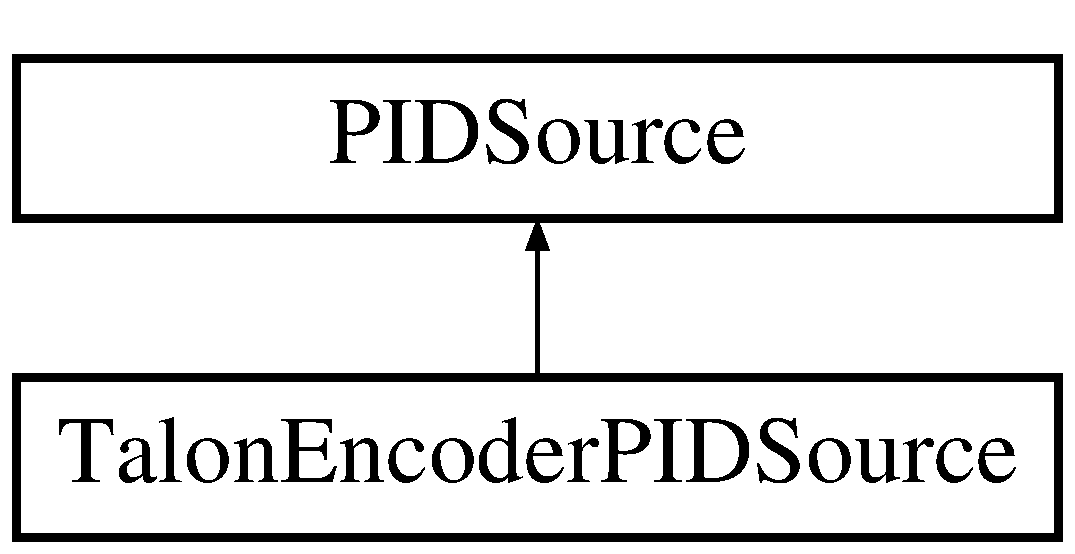
\includegraphics[height=2.000000cm]{class_talon_encoder_p_i_d_source}
\end{center}
\end{figure}
\subsection*{Public Member Functions}
\begin{DoxyCompactItemize}
\item 
\mbox{\Hypertarget{class_talon_encoder_p_i_d_source_a28f25e0a00329e64f15709b598dc0eda}\label{class_talon_encoder_p_i_d_source_a28f25e0a00329e64f15709b598dc0eda}} 
{\bfseries Talon\+Encoder\+P\+I\+D\+Source} (\hyperlink{class_robot_model}{Robot\+Model} $\ast$robot)
\item 
\mbox{\Hypertarget{class_talon_encoder_p_i_d_source_a0817f0ebd370ae8a6a00fd376d0840cb}\label{class_talon_encoder_p_i_d_source_a0817f0ebd370ae8a6a00fd376d0840cb}} 
double {\bfseries P\+I\+D\+Get} ()
\end{DoxyCompactItemize}
\subsection*{Private Attributes}
\begin{DoxyCompactItemize}
\item 
\mbox{\Hypertarget{class_talon_encoder_p_i_d_source_aa4e781ff25f6cb983fe40651b64f5f74}\label{class_talon_encoder_p_i_d_source_aa4e781ff25f6cb983fe40651b64f5f74}} 
\hyperlink{class_robot_model}{Robot\+Model} $\ast$ {\bfseries robot\+\_\+}
\item 
\mbox{\Hypertarget{class_talon_encoder_p_i_d_source_a7a1118cb2256b0d597f3e987c8062cf9}\label{class_talon_encoder_p_i_d_source_a7a1118cb2256b0d597f3e987c8062cf9}} 
double {\bfseries average\+Talon\+Distance\+\_\+}
\end{DoxyCompactItemize}


The documentation for this class was generated from the following files\+:\begin{DoxyCompactItemize}
\item 
/\+Users/maggiewang/\+Space\+\_\+\+Cookies/spacecookies/frc2017/src/\+Auto/P\+I\+D\+Input\+Source.\+h\item 
/\+Users/maggiewang/\+Space\+\_\+\+Cookies/spacecookies/frc2017/src/\+Auto/P\+I\+D\+Input\+Source.\+cpp\end{DoxyCompactItemize}

\hypertarget{class_test_mode}{}\section{Test\+Mode Class Reference}
\label{class_test_mode}\index{Test\+Mode@{Test\+Mode}}


The documentation for this class was generated from the following files\+:\begin{DoxyCompactItemize}
\item 
/\+Users/maggiewang/\+Space\+\_\+\+Cookies/spacecookies/frc2017/src/\+Auto/\+Modes/Test\+Mode.\+h\item 
/\+Users/maggiewang/\+Space\+\_\+\+Cookies/spacecookies/frc2017/src/\+Auto/\+Modes/Test\+Mode.\+cpp\end{DoxyCompactItemize}

\hypertarget{class_toggle_button_reader}{}\section{Toggle\+Button\+Reader Class Reference}
\label{class_toggle_button_reader}\index{Toggle\+Button\+Reader@{Toggle\+Button\+Reader}}
Inheritance diagram for Toggle\+Button\+Reader\+:\begin{figure}[H]
\begin{center}
\leavevmode
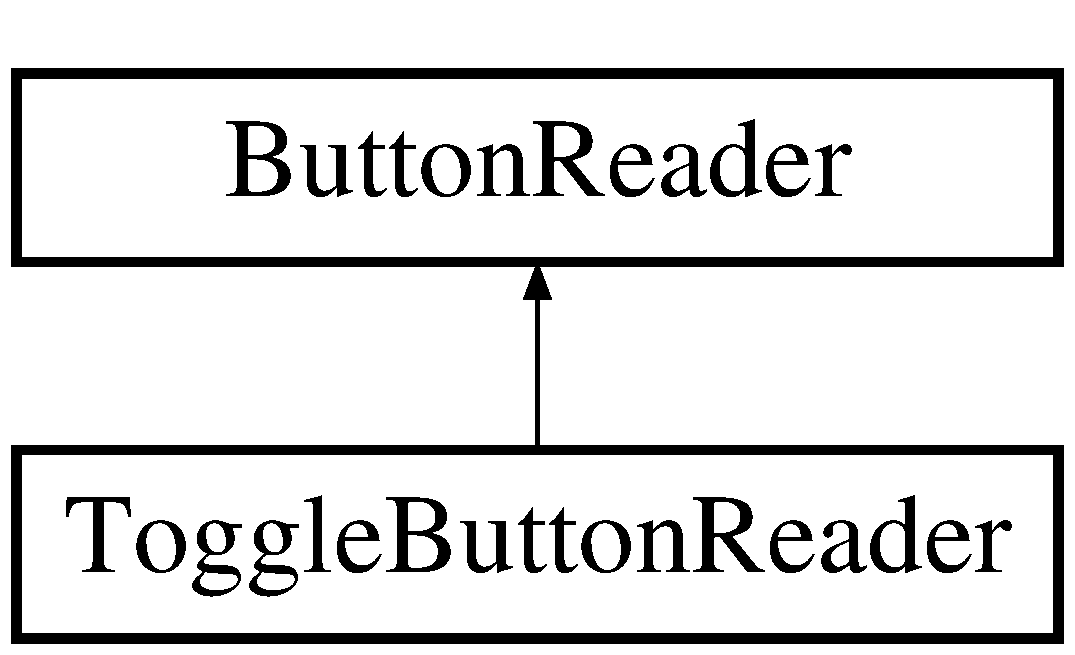
\includegraphics[height=2.000000cm]{class_toggle_button_reader}
\end{center}
\end{figure}
\subsection*{Public Member Functions}
\begin{DoxyCompactItemize}
\item 
\mbox{\Hypertarget{class_toggle_button_reader_af843241ff4ac0ce1c7806b910465b082}\label{class_toggle_button_reader_af843241ff4ac0ce1c7806b910465b082}} 
{\bfseries Toggle\+Button\+Reader} (Joystick $\ast$joy, int button\+Num)
\item 
\mbox{\Hypertarget{class_toggle_button_reader_a9141b60884e4fcef08d8bde89155feff}\label{class_toggle_button_reader_a9141b60884e4fcef08d8bde89155feff}} 
virtual bool {\bfseries Get\+State} ()
\end{DoxyCompactItemize}
\subsection*{Private Attributes}
\begin{DoxyCompactItemize}
\item 
\mbox{\Hypertarget{class_toggle_button_reader_a32f620dffec59210d1d90c747a41d5d6}\label{class_toggle_button_reader_a32f620dffec59210d1d90c747a41d5d6}} 
bool {\bfseries curr\+Toggle\+State}
\end{DoxyCompactItemize}


The documentation for this class was generated from the following files\+:\begin{DoxyCompactItemize}
\item 
/\+Users/maggiewang/\+Space\+\_\+\+Cookies/spacecookies/frc2017/src/\+Driver\+Station/Button\+Reader.\+h\item 
/\+Users/maggiewang/\+Space\+\_\+\+Cookies/spacecookies/frc2017/src/\+Driver\+Station/Button\+Reader.\+cpp\end{DoxyCompactItemize}

\hypertarget{class_z_m_q_test}{}\section{Z\+M\+Q\+Test Class Reference}
\label{class_z_m_q_test}\index{Z\+M\+Q\+Test@{Z\+M\+Q\+Test}}
\subsection*{Public Member Functions}
\begin{DoxyCompactItemize}
\item 
\mbox{\Hypertarget{class_z_m_q_test_ac1faea32929d288af0c9dcaf13322f44}\label{class_z_m_q_test_ac1faea32929d288af0c9dcaf13322f44}} 
void {\bfseries Update} ()
\end{DoxyCompactItemize}
\subsection*{Private Attributes}
\begin{DoxyCompactItemize}
\item 
\mbox{\Hypertarget{class_z_m_q_test_a02d8adadf7024abd80076a746d5ddefc}\label{class_z_m_q_test_a02d8adadf7024abd80076a746d5ddefc}} 
zmq\+::context\+\_\+t $\ast$ {\bfseries context}
\item 
\mbox{\Hypertarget{class_z_m_q_test_a4d4191d10f215c75f40e536cdd86f09b}\label{class_z_m_q_test_a4d4191d10f215c75f40e536cdd86f09b}} 
zmq\+::socket\+\_\+t $\ast$ {\bfseries subscriber}
\end{DoxyCompactItemize}


The documentation for this class was generated from the following files\+:\begin{DoxyCompactItemize}
\item 
/\+Users/maggiewang/\+Space\+\_\+\+Cookies/spacecookies/frc2017/src/\+Auto/\+Vision/Z\+M\+Q\+Test.\+h\item 
/\+Users/maggiewang/\+Space\+\_\+\+Cookies/spacecookies/frc2017/src/\+Auto/\+Vision/Z\+M\+Q\+Test.\+cpp\end{DoxyCompactItemize}

%--- End generated contents ---

% Index
\backmatter
\newpage
\phantomsection
\clearemptydoublepage
\addcontentsline{toc}{chapter}{Index}
\printindex

\end{document}
